\section{Modules}
In this chapter we introduce the concept of modules. Modules over a ring are a generalization of abelian groups (which are modules over $\mathbb{Z}$), where another proof of the factorization of finitely generated abelian groups is developed. The concept of modules are basic in the further study of algebra.
\subsection{Modules, Homomorphisms and Exact Sequences}
We first give the definition of a module.
\begin{definition}
Let $R$ be a ring, a (left) \textbf{$R$-module} is an additive abelian group $A$ together with a function $f:R\times A\to A$ (the image of $(r,a)$ is denoted as $ra$) such that for all $r,s\in R$ and $a,b\in A$ \par
(i) $r(a+b)=ra+rb$;\par
(ii) $(r+s)a=ra+sa$;\par
(iii) $r(sa)=(rs)a$.\par
If $R$ has an identity element $1_R$ and \par
(iv) $1_Ra=a$ for all $a\in A$,\par
then $A$ is said to be a \textbf{unitary $R$-module}. If $R$ is a division ring, then a unitary $R$-module is called a (left) vector space.
\end{definition}
A unitary right $R$-module is defined similarly via a function $A\times R\to A$ denoted $(a,r)\mapsto ar$ and satisfying the obvious analogous (i) to (iv). From now on, unless specified otherwise, $R$-module means left $R$-module and it is understood that all theorems about left $R$-modules also hold, \textit{mutatis mutandis}, for right $R$-modules.\par
A given group $A$ may have many different $R$-module structures. If $R$ is commutative, it is easy to verify that every left $R$-module $A$ can be given on the structure of a right $R$-module by defining $ar=ra$ for all $r\in R,a\in A$, where commutativity is needed in (iii). Now every module $A$ over a commutative ring $R$ is considered to be both left and right with $ar=ra$ for all $a\in A$ and $r\in R$.\par
\begin{example}\em
Every additive abelian group $G$ is a unitary $\mathbb{Z}$-module, with $na$ ($n\in\mathbb{Z}$ and $a\in G$) given by the usual definition for groups.
\end{example}
\begin{example}\em
If $S$ is a ring and $R$ is a subring of $S$, then $S$ is an $R$-module (but not vice versa) with $ra$ being multiplication on $S$. In particular, the polynomial ring $R[x_1,\cdots,x_n]$ and the formal power series ring $R[[x]]$ are $R$-modules.
\end{example}
\begin{example}\em
Let $R$ be a ring and $I$ be a left ideal of $R$. Then $I$ is an $R$-module with $ra\in I$ for all $r\in R$ and $a\in I$ under multiplication of $R$. In particular, $0$ and $R$ are trivial $R$-modules. Furthermore, since $I$ is an additive group, we have $R/I$ be an (abelian) group and an $R$-module with $r(r_1+I)=rr_1+I$. Note that $R/I$ need not to be a ring, unless $I$ is a two-sided ideal.
\end{example}
\begin{example}\em
Let $\varphi:R\to S$ be a ring homomorphism and let $A$ be an $S$-module. Then $A$ can be made into an $R$-module by defining $rx$ to be $\varphi(r)x$, where $r\in R$ and $x\in A$. One says that the $R$-module structure of $A$ is given by \textbf{pullback along $\varphi$}.
\end{example}
\begin{example}\em
Let $A$ be an abelian group and $\mathrm{End}A$ be its endomorphism ring. Then $A$ is a unitary $\mathrm{End}A$-module with $fa$ defined to be $f(a)$, where $a\in A$ and $f\in\mathrm{End}A$.
\end{example}
\begin{example}\em
If $R$ is a ring, every abelian group can be made into an $R$-module with trivial structure with $ra=0$ for all $r\in R$ and $a\in A$.
\end{example}
\begin{definition}
Let $A$ and $B$ be modules over a ring $R$. A function $f:A\to B$ is an \textbf{$R$-module homomorphism} provided that for all $a,c\in A$ and $r\in R$ we have $f(a+c)=f(a)+f(c)$ and $f(ra)=rf(a)$. If $R$ is a division ring, then an $R$-module homomorphism is called a \textbf{linear transformation}.
\end{definition}
When the context is clear we call an $R$-module homomorphism simply a homomorphism. By definition every $R$-module homomorphism is a homomorphism of abelian groups $A\to B$. Therefore the terminologies are used: an $R$-module homomorphism $f$ is an epimorphism [resp. monomorphism, isomorphism] if and only if $f$ is surjective [resp. injective, bijective] as a map of sets. The \textbf{kernel} of $f$ is its kernel as abelian groups, i.e. $\mathrm{Ker}f=\{a\in A:f(a)=0\}$. The \textbf{image} of $f$ is the set $\mathrm{Im}f=\{b\in B:b=f(a)\ \text{for some}\ a\in A\}$. We have the following propositions:
\begin{proposition}
$f$ is an $R$-module monomorphism [resp. isomorphism] if and only if $\mathrm{Ker}f=0$ [resp. there exists some $g:B\to A$ such that $fg=1_B$ and $gf=1_A$].
\end{proposition}
For a proof of this proposition, see Theorem 2.9. We now give some examples of homomorphisms of modules.
\begin{example}\em
For any modules the zero map $0:A\to B$ given by $a\mapsto 0$ is a trivial homomorphism. Every homomorphism of abelian groups is a homomorphism of $\mathbb{Z}$-module. If $R$ is a ring, then the map $R[x]\to R[x]$ given by $f\mapsto xf$ is a $R$-module homomorphism. Note that $f\mapsto xf$ is not a ring homomorphism.
\end{example}
Note that for a given ring $R$ the class of all $R$-modules [resp. unitary $R$-modules] and $R$-module homomorphisms clearly forms a (concrete) category.
\begin{definition}
Let $R$ be a ring, $A$ am $R$-module and $B$ a nonempty subset of $A$. $B$ is a \textbf{submodule} of $A$ provided that $B$ is an additive subgroup of $A$ and $rb\in B$ for all $r\in R$ and $b\in B$. A submodule of a vector space over a division ring is called a \textbf{subspace}.
\end{definition}
Note that a submodule itself is a module. Also a submodule of a unitary module over a ring with identity is necessarily unitary.
\begin{example}\em
Let $R$ be a ring and $f:A\to B$ is an $R$-module homomorphism, then $\mathrm{Ker}f$ is a submodule of $A$ and $\mathrm{Im}f$ is a submodule of $B$. If $C$ is a submodule of $B$, then $f^{-1}(C)$ is a submodule of $A$.
\end{example}
\begin{example}\em
If $R$ is a ring and $I$ is a left ideal of $R$, $A$ an $R$-module and $S$ a nonempty subset of $A$, then $IS=\left\{\sum_{i=1}^nr_ia_i:r_i\in I,a_i\in S,n\in\mathbb{N}_+\right\}$ is a submodule of $A$. Similarly if $a\in A$, then $Ia=\{ra:r\in I\}$ is a submodule of $A$.
\end{example}
\begin{example}\em
If $\{B_i:i\in I\}$ is a family of submodules of a module $A$, then $\bigcap_{i\in I}B_i$ is also a submodule of $A$.
\end{example}
\begin{definition}
If $X$ is a subset of a module $A$ over a ring $R$, then the intersection of all submodules of $A$ containing $X$ is called the \textbf{submodule generated by $X$} (or \textbf{spanned by $X$}).
\end{definition}
If $X$ is finite, and $X$ generates the module $B$, then $B$ is said to be \textbf{finitely generated}. If $X=\emptyset$, then $X$ clearly generates the zero module. If $X$ consists of a single element, i.e. $X=\{a\}$, then the submodule generated by $X$ is called the \textbf{cyclic (sub)module} generated by $a$. Finally, if $\{B_i:i\in I\}$ is a family of submodules of $A$, then the submodule generated by $X=\bigcup_{i\in I}B_i$ is called the \textbf{sum} of modules $B_i$. If the index is finite, the sum of $B_1,\cdots,B_n$ is denoted $B_1+B_2+\cdots+B_n$.\par
The next theorem gives some basic properties of submodules.
\begin{theorem}
Let $R$ be a ring, $A$ an $R$-module, $X$ a subset of $A$, $\{B_i:i\in I\}$ a family of submodules of $A$ and $a\in A$. Let $Ra=\{ra:r\in R\}$.\par
(i) $Ra$ is a submodule of $A$ and the map $R\to Ra$ given by $r\mapsto ra$ is an $R$-module epimorphism.\par
(ii) The cyclic submodule $C$ generated by $a$ is $\{ra+na:r\in R,n\in\mathbb{Z}\}$. If $R$ has an identity and $C$ is unitary, then $C=Ra$.\par
(iii) The submodule $D$ generated by $X$ is 
$$
\left\{ \sum_{i=1}^s{r_ia_i}+\sum_{j=1}^t{n_jb_j}:s,t\in \mathbb{N} _+,a_j,b_j\in X,r_i\in R,n_j\in \mathbb{Z} \right\} .
$$
If $R$ has an identity and $A$ is unitary, then 
$$
D=RX=\left\{ \sum_{i=1}^s{r_ia_i}:s\in \mathbb{N} _+,a_i\in X,r_i\in R \right\} .
$$\par
(iv) The sum of the family $\{B_i:i\in I\}$ consists of all finite sums $b_{i1}+\cdots+b_{in}$ with $b_{ik}\in B_{ik}$.
\end{theorem}
\begin{proof}
(i) We first show that $Ra$ is a submodule. Clearly $Ra$ is an abelian group. Now suppose $r\in R$ and $r^\prime a\in Ra$, then $rr^\prime a\in Ra$, whence $Ra$ is an $R$-submodule of $A$. Define $f:R\to Ra$ given by $r\mapsto ra$, then for all $ra\in Ra$ we have $f(r)=ra$, whence $f$ is an epimorphism.\par
(ii) It is easy to verify that $\{ra+na\}$ is a module over $R$. Suppose $A$ is the module generated by $a$, then $ra\in A$, $na\in A$. Therefore $ra+na\in A$, hence $\{ra+na\}$ is the smallest module generated by $a$, therefore $C=\{ra+na\}$. If $R$ has an identity and $R$ is a unitary module, then $na=(n1_R)a\in Ra$.\par
(iii) An similar proof to (ii) may be made to conclude the assertion. We skip the proof.\par
(iv) Since the sum of $\{B_i:i\in I\}$ is generated by all elements of $B_i$, therefore $b_{i1}+\cdots+b_{in}$ is an element of the module generated by all $B_i$.
\end{proof}
\begin{theorem}
Let $B$ be a submodule of a module $A$ over a ring $R$. Then the quotient group $A/B$ is an $R$-module with the action of $R$ on $A/B$ given by 
$$
r\left( a+B \right) =ra+B,r\in R,a\in A.
$$
The map $\pi:A\to A/B$ given by $a\mapsto a+B$ is an $R$-module epimorphism with kernel $B$.
\end{theorem}
\begin{proof}
We first show that the definitions here are well-defined. First, since $B$ is a submodule of $A$, then $B$ is an abelian group and $rb\in B$ for all $r\in R$ and $b\in B$. Therefore $B\lhd A$ and hence $A/B$ is well-defined. Now suppose $a+B=a^\prime+B$, then $a-a^\prime\in B$. Since $B$ is a module, then $r(a-a^\prime)\in B$ for all $r\in R$, whence $ra+B=ra^\prime+B$ and the action is well-defined. By definition it is easy to verify that $A/B$ is an $R$-module and $\pi$ is an epimorphism with $\mathrm{Ker}\pi=B$.
\end{proof}
\begin{note}\em
The map $\pi:A\to A/B$ is called the \textbf{canonical epimorphism} (or \textbf{projection}).
\end{note}
In view of the preceding results, it is not surprising that the various isomorphism theorems for groups are valid, \textit{mutatis mutandis}, for modules. One need only check at each stage of the proof to see that every subgroup of homomorphism is in fact a submodule or module homomorphism. We omit the results here. See Theorem 2.35 to Corollary 2.39.\par
Next we show that product and coproducts always exist in the category of $R$-modules.
\begin{theorem}
Let $R$ be a ring and $\{A_i:i\in I\}$ a nonempty family of $R$-modules, $\prod_{i\in I}A_i$ the direct product of the abelian groups $A_i$, and $\bigoplus_{i\in I}A_i$ the direct sum of the abelian groups $A_i$.\par
(i) $\prod_{i\in I}A_i$ is an $R$-module with the action of $R$ given by $r\{a_i\}=\{ra_i\}$.\par
(ii) $\bigoplus_{i\in I}A_i$ is a submodule of $\prod_{i\in I}A_i$.\par
(iii) For each $k\in I$, the canonical projection $\pi_k:\prod A_i\to A_k$ is an $R$-module epimorphism.\par
(iv) For each $k\in I$, the canonical injection $\iota_k:A_k\to\bigoplus A_i$ is an $R$-module monomorphism.
\end{theorem}
\begin{proof}
(i) Trivially $\prod A_i$ is an abelian group. By definition we have $A_i$ is an $R$-module, and hence $ra_i\in A_i$ for all $i\in I$. Therefore $r\{a_i\}=\{ra_i\}\in\prod A_i$ and hence $\prod A_i$ is an $R$-module with the given action.\par
(ii) By definition $\bigoplus A_i$ is a subgroup of $\prod A_i$. Note that for all $r\in R$ and $\{a_i\}_{i\in I}\in\bigoplus A_i$ we have $r\{a_i\}=\{ra_i\}\in\bigoplus A_i$, therefore $\bigoplus A_i$ is a submodule of $\prod A_i$.\par
(iii) and (iv) See section 2.8.
\end{proof}
$\prod A_i$ is called the (external) \textbf{direct product} of the family of $R$-modules $\{A_i:i\in I\}$ and $\bigoplus A_i$ is its (external) \textbf{direct sum}. If the index is finite, say $I=\{1,2,\cdots,n\}$, then the direct product and the direct sum coincide and will be written $A_1\oplus A_2\oplus\cdots\oplus A_n$. The maps $\pi_k$ [resp. $\iota_k$] are called the \textbf{canonical projections} [resp. \textbf{injections}]. Clearly, $\prod A_i$ and $\bigoplus A_i$ has the universal properties and is determined uniquely by this property.\par
Finite direct sums occur so frequently that a further discussion of them will be useful. We first observe that if $f$ and $g$ are $R$-module homomorphisms from an $R$-module $A$ to another $R$-module $B$, then the map $f+g:A\to B$ given by $a+b\mapsto f(a)+f(b)$ is also an $R$-module homomorphism. It is easy to verify that the set $\mathrm{Hom}_R(A,B)$ of all homomorphisms of $A$ to $B$ is an abelian group under the addition. Furthermore addition of module homomorphisms is distributive with respect to composition of functions, i.e. $h(f+g)=hf+hg$ and $(f+g)k=fk+gk$, where $f,g:A\to B$ and $h:B\to C$, $k:D\to A$.
\begin{theorem}
Let $R$ be a ring and $A_1,\cdots,A_n$ be $R$-modules. Then $A\cong A_1\oplus\cdots\oplus A_n$ if and only if for each $i=1,2,\cdots,n$ there are $R$-module homomorphisms $\pi_i:A\to A_i$, $\iota_i:A_i\to A$ such that \par
(i) $\pi_i\iota_i=1_{A_{i}}$ for all $i=1,2,\cdots,n$;\par
(ii) $\pi_j\iota_i=0$ for $i\ne j$;\par
(iii) $\iota_1\pi_1+\cdots+\iota_n\pi_n=1_A$.
\end{theorem}
\begin{proof}
To show the existence of $\pi_i$ and $\iota_i$, consider the canonical injections and canonical projections. Conversely, if there exists $\pi_i$ and $\iota_i$ satisfies (i), (ii) and (iii), then consider canonical injections $\pi_i^\prime$ and canonical projections $\iota_i^\prime$. Let $\varphi:A_1\oplus A_2\oplus\cdots\oplus A_n$ and $\psi:A\to A_1\oplus A_2\oplus\cdots\oplus A_n$ by $\iota_1^\prime\pi_1+\cdots+\iota_n^\prime\pi_n$, we have 
$$
\varphi \psi =\left( \sum_{i=1}^n{\iota _i\pi _{i}^{\prime}} \right) \left( \sum_{i=1}^n{\iota _{i}^{\prime}\pi _i} \right) =\sum_{i=1}^n{\sum_{j=1}^n{\iota _{i}^{\prime}\pi _i}\iota _j\pi _{j}^{\prime}}=\sum_{i=1}^n{\iota _i1_{A_i}\pi _i}=\sum_{i=1}^n{\iota _i\pi _i}=1_A,
$$
and similarly 
$$
\psi \varphi =\left( \sum_{i=1}^n{\iota _{i}^{\prime}\pi _i} \right) \left( \sum_{i=1}^n{\iota _i\pi _{i}^{\prime}} \right) =\sum_{i=1}^n{\sum_{i=1}^n{\iota _i\pi _{i}^{\prime}}\iota _{i}^{\prime}\pi _i}=1_{A_1\oplus A_2\oplus \cdots \oplus A_n}.
$$
Therefore $\varphi$ is an isomorphism and the proof is finished.
\end{proof}
\begin{theorem}
Let $R$ be a ring and $\{A_i:i\in I\}$ a family of submodules of an $R$-module $A$ such that $A$ is the sum of the family $\{A_i:i\in I\}$, and for each $k\in I$ we have $A_k\cap A_k^*=0$, where $A_k^*=\{A_i:i\ne k\}$, then there is an isomorphism $A\cong\bigoplus_{i\in I}A_i$.
\end{theorem}
The proof of this theorem may be referred to Theorem 2.68.\par
Note that there are also similar concepts of \textbf{internal direct product}, which is, indeed, isomorphic to the external direct product introduced before. However, note that the internal direct product of $\{A_i:i\in I\}$ does not actually contain $A_i$'s but only isomorphic pieces of it. The adjective internal and external are omitted when no confusion will be made in context.\par
We now introduce another important concept, which is very useful in homomorphic algebra: 
\begin{definition}
A pair of module homomorphisms, $A\overset{f}{\longrightarrow}B\overset{g}{\longrightarrow}C$, is said to be \textbf{exact} at $B$ provided $\mathrm{Im}f=\mathrm{Ker}g$. A finite sequence of module homomorphisms, $A_0\overset{f_1}{\longrightarrow}A_1\overset{f_2}{\longrightarrow}\cdots \overset{f_{n-1}}{\longrightarrow}A_{n-1}\overset{f_n}{\longrightarrow}A_n$, is \textbf{exact} provided $\mathrm{Im}f_i=\mathrm{Ker}f_{i+1}$ for $i=1,2,\cdots,n-1$. An infinite sequence of module homomorphisms, $\cdots \overset{f_{i-1}}{\longrightarrow}A_{i-1}\overset{f_i}{\longrightarrow}A_i\overset{f_{i+1}}{\longrightarrow}A_{i+1}\overset{f_{i+2}}{\longrightarrow}\cdots $ is \textbf{exact} provided $\mathrm{Im}f_i=\mathrm{Ker}f_{i+1}$ for all $i\in\mathbb{Z}$.
\end{definition}
When convenience we shall abuse the language slightly and refer to an exact sequence of modules rather than an exact sequence of module homomorphisms.
\begin{example}\em
Note first that for any module $A$, there are unique module homomorphisms $0\longrightarrow A$ and $A\longrightarrow 0$. If $A$ and $B$ are modules then the sequences $0\longrightarrow A\overset{\iota}{\longrightarrow}A\oplus B\overset{\pi}{\longrightarrow}B\longrightarrow 0$ and $0\longrightarrow B\overset{\iota}{\longrightarrow}A\oplus B\overset{\pi}{\longrightarrow}A\longrightarrow 0$ are exact, where the $\iota$'s and $\pi$'s are the canonical injections and projections respectively. Similarly, if $C$ is a submodule of $D$, then the sequence $0\longrightarrow C\overset{i}{\longrightarrow}D\overset{p}{\longrightarrow}D/C\longrightarrow 0$ is exact, there $i$ and $p$ are trivial injection and projection. If $f:A\to B$ is a module homomorphism, then $A/\mathrm{Ker}f$ [resp. $B/\mathrm{Im}f$] is called the \textbf{coimage} of $f$ [resp. \textbf{cokernel} of $f$] and denote as $\mathrm{CoIm}f$ [resp. $\mathrm{CoKer}f$]. Each of the following sequences is exact: $0\longrightarrow \mathrm{Ker}f\longrightarrow A\longrightarrow \mathrm{CoIm}f\longrightarrow 0$, $0\longrightarrow \mathrm{Im}f\longrightarrow B\longrightarrow \mathrm{CoKer}f\longrightarrow 0$ and $0\longrightarrow \mathrm{Ker}f\longrightarrow A\longrightarrow B\longrightarrow \mathrm{CoKer}f\longrightarrow 0$.
\end{example}
\begin{note}\em
$0\longrightarrow A\overset{f}{\longrightarrow}B$ is an exact sequence of module homomorphism if and only if $f$ is a module monomorphism. Similarly, $B\overset{g}{\longrightarrow}C\longrightarrow 0$ is exact if and only if $g$ is a module epimorphism. If $A\overset{f}{\longrightarrow}B\overset{g}{\longrightarrow}C$ is exact, then $gf=0$. Finally if $A\overset{f}{\longrightarrow}B\overset{g}{\longrightarrow}C\longrightarrow 0$ is exact, then 
$$
\mathrm{CoKer}f=B/\mathrm{Im}f=B/\mathrm{Ker}g=\mathrm{CoIm}g\cong C.
$$
An exact sequence of the form $0\longrightarrow A\overset{f}{\longrightarrow}B\overset{g}{\longrightarrow}C\longrightarrow 0$ is called a \textbf{short exact sequence}. Note that $f$ is a monomorphism and $g$ an epimorphism. The preceding remarks show that a short exact sequence is just another way of presenting a submodule ($A\cong\mathrm{Im}f$) and its quotient module ($B/\mathrm{Im}f=B/\mathrm{Ker}g\cong C$).
\end{note}
\begin{lemma}\em(The Short Five Lemma)
Let $R$ be a ring and 
\begin{center}


\tikzset{every picture/.style={line width=0.75pt}} %set default line width to 0.75pt        

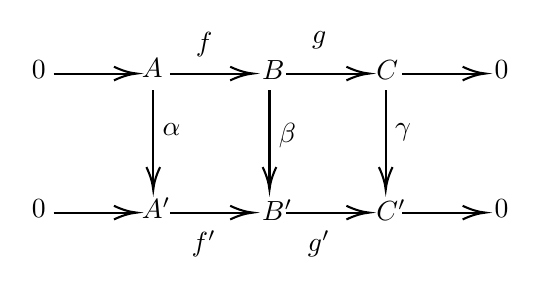
\begin{tikzpicture}[x=0.75pt,y=0.75pt,yscale=-1,xscale=1]
%uncomment if require: \path (0,476); %set diagram left start at 0, and has height of 476

%Straight Lines [id:da22573280049285005] 
\draw    (160,224) -- (198,224) ;
\draw [shift={(200,224)}, rotate = 180] [color={rgb, 255:red, 0; green, 0; blue, 0 }  ][line width=0.75]    (10.93,-3.29) .. controls (6.95,-1.4) and (3.31,-0.3) .. (0,0) .. controls (3.31,0.3) and (6.95,1.4) .. (10.93,3.29)   ;
%Straight Lines [id:da5007083409135236] 
\draw    (216,224) -- (254,224) ;
\draw [shift={(256,224)}, rotate = 180] [color={rgb, 255:red, 0; green, 0; blue, 0 }  ][line width=0.75]    (10.93,-3.29) .. controls (6.95,-1.4) and (3.31,-0.3) .. (0,0) .. controls (3.31,0.3) and (6.95,1.4) .. (10.93,3.29)   ;
%Straight Lines [id:da49627755138453633] 
\draw    (272,224) -- (310,224) ;
\draw [shift={(312,224)}, rotate = 180] [color={rgb, 255:red, 0; green, 0; blue, 0 }  ][line width=0.75]    (10.93,-3.29) .. controls (6.95,-1.4) and (3.31,-0.3) .. (0,0) .. controls (3.31,0.3) and (6.95,1.4) .. (10.93,3.29)   ;
%Straight Lines [id:da7229825431747845] 
\draw    (328,224) -- (366,224) ;
\draw [shift={(368,224)}, rotate = 180] [color={rgb, 255:red, 0; green, 0; blue, 0 }  ][line width=0.75]    (10.93,-3.29) .. controls (6.95,-1.4) and (3.31,-0.3) .. (0,0) .. controls (3.31,0.3) and (6.95,1.4) .. (10.93,3.29)   ;
%Straight Lines [id:da42771610429371165] 
\draw    (160,291) -- (198,291) ;
\draw [shift={(200,291)}, rotate = 180] [color={rgb, 255:red, 0; green, 0; blue, 0 }  ][line width=0.75]    (10.93,-3.29) .. controls (6.95,-1.4) and (3.31,-0.3) .. (0,0) .. controls (3.31,0.3) and (6.95,1.4) .. (10.93,3.29)   ;
%Straight Lines [id:da12408345309174651] 
\draw    (216,291) -- (254,291) ;
\draw [shift={(256,291)}, rotate = 180] [color={rgb, 255:red, 0; green, 0; blue, 0 }  ][line width=0.75]    (10.93,-3.29) .. controls (6.95,-1.4) and (3.31,-0.3) .. (0,0) .. controls (3.31,0.3) and (6.95,1.4) .. (10.93,3.29)   ;
%Straight Lines [id:da5038313801743268] 
\draw    (272,291) -- (310,291) ;
\draw [shift={(312,291)}, rotate = 180] [color={rgb, 255:red, 0; green, 0; blue, 0 }  ][line width=0.75]    (10.93,-3.29) .. controls (6.95,-1.4) and (3.31,-0.3) .. (0,0) .. controls (3.31,0.3) and (6.95,1.4) .. (10.93,3.29)   ;
%Straight Lines [id:da8627554494400742] 
\draw    (328,291) -- (366,291) ;
\draw [shift={(368,291)}, rotate = 180] [color={rgb, 255:red, 0; green, 0; blue, 0 }  ][line width=0.75]    (10.93,-3.29) .. controls (6.95,-1.4) and (3.31,-0.3) .. (0,0) .. controls (3.31,0.3) and (6.95,1.4) .. (10.93,3.29)   ;
%Straight Lines [id:da9219190287457819] 
\draw    (208,232) -- (208,278) ;
\draw [shift={(208,280)}, rotate = 270] [color={rgb, 255:red, 0; green, 0; blue, 0 }  ][line width=0.75]    (10.93,-3.29) .. controls (6.95,-1.4) and (3.31,-0.3) .. (0,0) .. controls (3.31,0.3) and (6.95,1.4) .. (10.93,3.29)   ;
%Straight Lines [id:da4241610695219813] 
\draw    (264,232) -- (264,278) ;
\draw [shift={(264,280)}, rotate = 270] [color={rgb, 255:red, 0; green, 0; blue, 0 }  ][line width=0.75]    (10.93,-3.29) .. controls (6.95,-1.4) and (3.31,-0.3) .. (0,0) .. controls (3.31,0.3) and (6.95,1.4) .. (10.93,3.29)   ;
%Straight Lines [id:da5742073517286415] 
\draw    (320,232) -- (320,278) ;
\draw [shift={(320,280)}, rotate = 270] [color={rgb, 255:red, 0; green, 0; blue, 0 }  ][line width=0.75]    (10.93,-3.29) .. controls (6.95,-1.4) and (3.31,-0.3) .. (0,0) .. controls (3.31,0.3) and (6.95,1.4) .. (10.93,3.29)   ;

% Text Node
\draw (148,216.4) node [anchor=north west][inner sep=0.75pt]    {$0$};
% Text Node
\draw (201,215.4) node [anchor=north west][inner sep=0.75pt]    {$A$};
% Text Node
\draw (259,216.4) node [anchor=north west][inner sep=0.75pt]    {$B$};
% Text Node
\draw (314,216.4) node [anchor=north west][inner sep=0.75pt]    {$C$};
% Text Node
\draw (371,216.4) node [anchor=north west][inner sep=0.75pt]    {$0$};
% Text Node
\draw (148,283.4) node [anchor=north west][inner sep=0.75pt]    {$0$};
% Text Node
\draw (201,282.4) node [anchor=north west][inner sep=0.75pt]    {$A^{\prime }$};
% Text Node
\draw (259,283.4) node [anchor=north west][inner sep=0.75pt]    {$B^{\prime }$};
% Text Node
\draw (314,283.4) node [anchor=north west][inner sep=0.75pt]    {$C^{\prime }$};
% Text Node
\draw (371,283.4) node [anchor=north west][inner sep=0.75pt]    {$0$};
% Text Node
\draw (227,202.4) node [anchor=north west][inner sep=0.75pt]    {$f$};
% Text Node
\draw (283,202.4) node [anchor=north west][inner sep=0.75pt]    {$g$};
% Text Node
\draw (225,298.4) node [anchor=north west][inner sep=0.75pt]    {$f^{\prime }$};
% Text Node
\draw (281,298.4) node [anchor=north west][inner sep=0.75pt]    {$g^{\prime }$};
% Text Node
\draw (211,246.4) node [anchor=north west][inner sep=0.75pt]    {$\alpha $};
% Text Node
\draw (267,246.4) node [anchor=north west][inner sep=0.75pt]    {$\beta $};
% Text Node
\draw (323,246.4) node [anchor=north west][inner sep=0.75pt]    {$\gamma $};


\end{tikzpicture}
\end{center}
a commutative diagram of $R$-modules and $R$-module homomorphisms such that each row is a short exact sequence. Then \par
(i) $\alpha,\gamma$ monomorphisms implies $\beta$ monomorphism;\par
(ii) $\alpha,\gamma$ epimorphisms implies $\beta$ epimorphism;\par
(iii) $\alpha,\gamma$ isomorphisms implies $\beta$ isomorphism.
\end{lemma}
\begin{proof}
(i) Suppose $\beta(b)=0$, we show that $b=0$. Observe that $g^{\prime}\circ \beta \left( b \right) =\gamma \circ g\left( b \right) =0$ we have $g(b)\in\mathrm{Ker}\gamma$. However $\gamma$ is a monomorphism and hence $\mathrm{Ker}\gamma=0$, therefore $g(b)=0$. Since the first row is exact we have $\mathrm{Ker}g=\mathrm{Im}f$, therefore there exists some $a\in A$ such that $f(a)=b$. Note that $\beta \circ f\left( a \right) =f^{\prime}\circ \alpha \left( a \right) =0$, we have $\alpha(a)\in\mathrm{Ker}f$. However $\mathrm{Ker}f=0$, we have $a=0$ and hence $b=f(a)=0$, therefore $\beta$ is a monomorphism.\par
(ii) Let $b^\prime\in B$, then $g^\prime(b)=c^\prime\in C^\prime$. Since $\gamma$ is an epimorphism, there exists some $c\in C$ such that $\gamma(c)=c^\prime$. Also suppose $g(b)=c$. Therefore $c^{\prime}=g^{\prime}\circ \beta \left( b \right) =\gamma \circ g\left( b \right) =\gamma \left( c \right) =g^{\prime}\left( b^{\prime} \right) $ and hence $g^\prime[\beta(b)-b^\prime]=0$ and $\beta(b)-b^\prime\in\mathrm{Ker}g^\prime$. Since the bottom row is exact we have $\mathrm{Ker}g^\prime=\mathrm{Im}f^\prime$ and hence there exists some $a^\prime\in A^\prime$ such that $f^\prime(a^\prime)=\beta(b)-b^\prime$. Since $\alpha$ is an epimorphism let $a^\prime=\alpha(a)$ for some $a\in A$. Consider $b-f(a)\in B$, we have 
$$
\beta \left[ b-f\left( a \right) \right] =\beta \left( b \right) -\beta \circ f\left( a \right) =\beta \left( b \right) -\beta \left( b \right) +b^{\prime}=b^{\prime},
$$
which finished the proof.\par
(iii) By (i) and (ii), the condition is trivial.
\end{proof}
Two short exact sequences are said to be \textbf{isomorphic} if there is a commutative diagram of module homomorphisms 
\begin{center}


\tikzset{every picture/.style={line width=0.75pt}} %set default line width to 0.75pt        

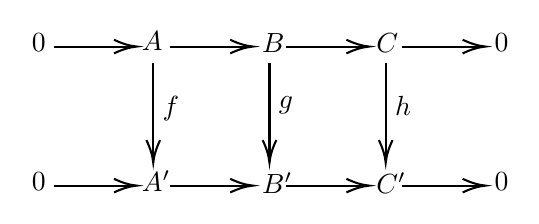
\begin{tikzpicture}[x=0.75pt,y=0.75pt,yscale=-1,xscale=1]
%uncomment if require: \path (0,476); %set diagram left start at 0, and has height of 476

%Straight Lines [id:da22573280049285005] 
\draw    (160,224) -- (198,224) ;
\draw [shift={(200,224)}, rotate = 180] [color={rgb, 255:red, 0; green, 0; blue, 0 }  ][line width=0.75]    (10.93,-3.29) .. controls (6.95,-1.4) and (3.31,-0.3) .. (0,0) .. controls (3.31,0.3) and (6.95,1.4) .. (10.93,3.29)   ;
%Straight Lines [id:da5007083409135236] 
\draw    (216,224) -- (254,224) ;
\draw [shift={(256,224)}, rotate = 180] [color={rgb, 255:red, 0; green, 0; blue, 0 }  ][line width=0.75]    (10.93,-3.29) .. controls (6.95,-1.4) and (3.31,-0.3) .. (0,0) .. controls (3.31,0.3) and (6.95,1.4) .. (10.93,3.29)   ;
%Straight Lines [id:da49627755138453633] 
\draw    (272,224) -- (310,224) ;
\draw [shift={(312,224)}, rotate = 180] [color={rgb, 255:red, 0; green, 0; blue, 0 }  ][line width=0.75]    (10.93,-3.29) .. controls (6.95,-1.4) and (3.31,-0.3) .. (0,0) .. controls (3.31,0.3) and (6.95,1.4) .. (10.93,3.29)   ;
%Straight Lines [id:da7229825431747845] 
\draw    (328,224) -- (366,224) ;
\draw [shift={(368,224)}, rotate = 180] [color={rgb, 255:red, 0; green, 0; blue, 0 }  ][line width=0.75]    (10.93,-3.29) .. controls (6.95,-1.4) and (3.31,-0.3) .. (0,0) .. controls (3.31,0.3) and (6.95,1.4) .. (10.93,3.29)   ;
%Straight Lines [id:da42771610429371165] 
\draw    (160,291) -- (198,291) ;
\draw [shift={(200,291)}, rotate = 180] [color={rgb, 255:red, 0; green, 0; blue, 0 }  ][line width=0.75]    (10.93,-3.29) .. controls (6.95,-1.4) and (3.31,-0.3) .. (0,0) .. controls (3.31,0.3) and (6.95,1.4) .. (10.93,3.29)   ;
%Straight Lines [id:da12408345309174651] 
\draw    (216,291) -- (254,291) ;
\draw [shift={(256,291)}, rotate = 180] [color={rgb, 255:red, 0; green, 0; blue, 0 }  ][line width=0.75]    (10.93,-3.29) .. controls (6.95,-1.4) and (3.31,-0.3) .. (0,0) .. controls (3.31,0.3) and (6.95,1.4) .. (10.93,3.29)   ;
%Straight Lines [id:da5038313801743268] 
\draw    (272,291) -- (310,291) ;
\draw [shift={(312,291)}, rotate = 180] [color={rgb, 255:red, 0; green, 0; blue, 0 }  ][line width=0.75]    (10.93,-3.29) .. controls (6.95,-1.4) and (3.31,-0.3) .. (0,0) .. controls (3.31,0.3) and (6.95,1.4) .. (10.93,3.29)   ;
%Straight Lines [id:da8627554494400742] 
\draw    (328,291) -- (366,291) ;
\draw [shift={(368,291)}, rotate = 180] [color={rgb, 255:red, 0; green, 0; blue, 0 }  ][line width=0.75]    (10.93,-3.29) .. controls (6.95,-1.4) and (3.31,-0.3) .. (0,0) .. controls (3.31,0.3) and (6.95,1.4) .. (10.93,3.29)   ;
%Straight Lines [id:da9219190287457819] 
\draw    (208,232) -- (208,278) ;
\draw [shift={(208,280)}, rotate = 270] [color={rgb, 255:red, 0; green, 0; blue, 0 }  ][line width=0.75]    (10.93,-3.29) .. controls (6.95,-1.4) and (3.31,-0.3) .. (0,0) .. controls (3.31,0.3) and (6.95,1.4) .. (10.93,3.29)   ;
%Straight Lines [id:da4241610695219813] 
\draw    (264,232) -- (264,278) ;
\draw [shift={(264,280)}, rotate = 270] [color={rgb, 255:red, 0; green, 0; blue, 0 }  ][line width=0.75]    (10.93,-3.29) .. controls (6.95,-1.4) and (3.31,-0.3) .. (0,0) .. controls (3.31,0.3) and (6.95,1.4) .. (10.93,3.29)   ;
%Straight Lines [id:da5742073517286415] 
\draw    (320,232) -- (320,278) ;
\draw [shift={(320,280)}, rotate = 270] [color={rgb, 255:red, 0; green, 0; blue, 0 }  ][line width=0.75]    (10.93,-3.29) .. controls (6.95,-1.4) and (3.31,-0.3) .. (0,0) .. controls (3.31,0.3) and (6.95,1.4) .. (10.93,3.29)   ;

% Text Node
\draw (148,216.4) node [anchor=north west][inner sep=0.75pt]    {$0$};
% Text Node
\draw (201,215.4) node [anchor=north west][inner sep=0.75pt]    {$A$};
% Text Node
\draw (259,216.4) node [anchor=north west][inner sep=0.75pt]    {$B$};
% Text Node
\draw (314,216.4) node [anchor=north west][inner sep=0.75pt]    {$C$};
% Text Node
\draw (371,216.4) node [anchor=north west][inner sep=0.75pt]    {$0$};
% Text Node
\draw (148,283.4) node [anchor=north west][inner sep=0.75pt]    {$0$};
% Text Node
\draw (201,282.4) node [anchor=north west][inner sep=0.75pt]    {$A^{\prime }$};
% Text Node
\draw (259,283.4) node [anchor=north west][inner sep=0.75pt]    {$B^{\prime }$};
% Text Node
\draw (314,283.4) node [anchor=north west][inner sep=0.75pt]    {$C^{\prime }$};
% Text Node
\draw (371,283.4) node [anchor=north west][inner sep=0.75pt]    {$0$};
% Text Node
\draw (211,246.4) node [anchor=north west][inner sep=0.75pt]    {$f$};
% Text Node
\draw (267,246.4) node [anchor=north west][inner sep=0.75pt]    {$g$};
% Text Node
\draw (323,246.4) node [anchor=north west][inner sep=0.75pt]    {$h$};


\end{tikzpicture}
\end{center}
such that $f,g$ and $h$ are isomorphisms. In this case, it is easy to verify that the diagram 
\begin{center}


\tikzset{every picture/.style={line width=0.75pt}} %set default line width to 0.75pt        

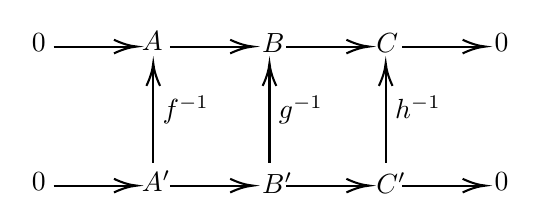
\begin{tikzpicture}[x=0.75pt,y=0.75pt,yscale=-1,xscale=1]
%uncomment if require: \path (0,476); %set diagram left start at 0, and has height of 476

%Straight Lines [id:da22573280049285005] 
\draw    (160,224) -- (198,224) ;
\draw [shift={(200,224)}, rotate = 180] [color={rgb, 255:red, 0; green, 0; blue, 0 }  ][line width=0.75]    (10.93,-3.29) .. controls (6.95,-1.4) and (3.31,-0.3) .. (0,0) .. controls (3.31,0.3) and (6.95,1.4) .. (10.93,3.29)   ;
%Straight Lines [id:da5007083409135236] 
\draw    (216,224) -- (254,224) ;
\draw [shift={(256,224)}, rotate = 180] [color={rgb, 255:red, 0; green, 0; blue, 0 }  ][line width=0.75]    (10.93,-3.29) .. controls (6.95,-1.4) and (3.31,-0.3) .. (0,0) .. controls (3.31,0.3) and (6.95,1.4) .. (10.93,3.29)   ;
%Straight Lines [id:da49627755138453633] 
\draw    (272,224) -- (310,224) ;
\draw [shift={(312,224)}, rotate = 180] [color={rgb, 255:red, 0; green, 0; blue, 0 }  ][line width=0.75]    (10.93,-3.29) .. controls (6.95,-1.4) and (3.31,-0.3) .. (0,0) .. controls (3.31,0.3) and (6.95,1.4) .. (10.93,3.29)   ;
%Straight Lines [id:da7229825431747845] 
\draw    (328,224) -- (366,224) ;
\draw [shift={(368,224)}, rotate = 180] [color={rgb, 255:red, 0; green, 0; blue, 0 }  ][line width=0.75]    (10.93,-3.29) .. controls (6.95,-1.4) and (3.31,-0.3) .. (0,0) .. controls (3.31,0.3) and (6.95,1.4) .. (10.93,3.29)   ;
%Straight Lines [id:da42771610429371165] 
\draw    (160,291) -- (198,291) ;
\draw [shift={(200,291)}, rotate = 180] [color={rgb, 255:red, 0; green, 0; blue, 0 }  ][line width=0.75]    (10.93,-3.29) .. controls (6.95,-1.4) and (3.31,-0.3) .. (0,0) .. controls (3.31,0.3) and (6.95,1.4) .. (10.93,3.29)   ;
%Straight Lines [id:da12408345309174651] 
\draw    (216,291) -- (254,291) ;
\draw [shift={(256,291)}, rotate = 180] [color={rgb, 255:red, 0; green, 0; blue, 0 }  ][line width=0.75]    (10.93,-3.29) .. controls (6.95,-1.4) and (3.31,-0.3) .. (0,0) .. controls (3.31,0.3) and (6.95,1.4) .. (10.93,3.29)   ;
%Straight Lines [id:da5038313801743268] 
\draw    (272,291) -- (310,291) ;
\draw [shift={(312,291)}, rotate = 180] [color={rgb, 255:red, 0; green, 0; blue, 0 }  ][line width=0.75]    (10.93,-3.29) .. controls (6.95,-1.4) and (3.31,-0.3) .. (0,0) .. controls (3.31,0.3) and (6.95,1.4) .. (10.93,3.29)   ;
%Straight Lines [id:da8627554494400742] 
\draw    (328,291) -- (366,291) ;
\draw [shift={(368,291)}, rotate = 180] [color={rgb, 255:red, 0; green, 0; blue, 0 }  ][line width=0.75]    (10.93,-3.29) .. controls (6.95,-1.4) and (3.31,-0.3) .. (0,0) .. controls (3.31,0.3) and (6.95,1.4) .. (10.93,3.29)   ;
%Straight Lines [id:da9219190287457819] 
\draw    (208,280) -- (208,234) ;
\draw [shift={(208,232)}, rotate = 90] [color={rgb, 255:red, 0; green, 0; blue, 0 }  ][line width=0.75]    (10.93,-3.29) .. controls (6.95,-1.4) and (3.31,-0.3) .. (0,0) .. controls (3.31,0.3) and (6.95,1.4) .. (10.93,3.29)   ;
%Straight Lines [id:da3968821204612032] 
\draw    (264,280) -- (264,234) ;
\draw [shift={(264,232)}, rotate = 90] [color={rgb, 255:red, 0; green, 0; blue, 0 }  ][line width=0.75]    (10.93,-3.29) .. controls (6.95,-1.4) and (3.31,-0.3) .. (0,0) .. controls (3.31,0.3) and (6.95,1.4) .. (10.93,3.29)   ;
%Straight Lines [id:da09148833810965606] 
\draw    (320,280) -- (320,234) ;
\draw [shift={(320,232)}, rotate = 90] [color={rgb, 255:red, 0; green, 0; blue, 0 }  ][line width=0.75]    (10.93,-3.29) .. controls (6.95,-1.4) and (3.31,-0.3) .. (0,0) .. controls (3.31,0.3) and (6.95,1.4) .. (10.93,3.29)   ;

% Text Node
\draw (148,216.4) node [anchor=north west][inner sep=0.75pt]    {$0$};
% Text Node
\draw (201,215.4) node [anchor=north west][inner sep=0.75pt]    {$A$};
% Text Node
\draw (259,216.4) node [anchor=north west][inner sep=0.75pt]    {$B$};
% Text Node
\draw (314,216.4) node [anchor=north west][inner sep=0.75pt]    {$C$};
% Text Node
\draw (371,216.4) node [anchor=north west][inner sep=0.75pt]    {$0$};
% Text Node
\draw (148,283.4) node [anchor=north west][inner sep=0.75pt]    {$0$};
% Text Node
\draw (201,282.4) node [anchor=north west][inner sep=0.75pt]    {$A^{\prime }$};
% Text Node
\draw (259,283.4) node [anchor=north west][inner sep=0.75pt]    {$B^{\prime }$};
% Text Node
\draw (314,283.4) node [anchor=north west][inner sep=0.75pt]    {$C^{\prime }$};
% Text Node
\draw (371,283.4) node [anchor=north west][inner sep=0.75pt]    {$0$};
% Text Node
\draw (211,246.4) node [anchor=north west][inner sep=0.75pt]    {$f^{-1}$};
% Text Node
\draw (267,246.4) node [anchor=north west][inner sep=0.75pt]    {$g^{-1}$};
% Text Node
\draw (323,246.4) node [anchor=north west][inner sep=0.75pt]    {$h^{-1}$};


\end{tikzpicture}
\end{center}
(with the same horizontal maps) is also commutative. In fact, isomorphism of short exact sequences is an equivalent relation.
\begin{theorem}
Let $R$ be a ring and $0\longrightarrow A_1\overset{f}{\longrightarrow}B\overset{g}{\longrightarrow}A_2\longrightarrow 0$ a short exact sequence of $R$-module homomorphisms. Then the following conditions are equivalent.\par
(i) There is an $R$-module homomorphism $h:A_2\to B$ with $gh=1_{A_2}$.\par
(ii) There is an $R$-module homomorphism $k:B\to A_1$ with $kf=1_{A_1}$.\par
(iii) The given sequence is isomorphic to the direct sum short exact sequence $0\longrightarrow A_1\overset{\iota _1}{\longrightarrow}A_1\oplus A_2\overset{\pi _2}{\longrightarrow}A_2\longrightarrow 0$. In particular $B\cong A_1\oplus A_2$.
\end{theorem}
\begin{proof}
(i)$\Rightarrow$(iii): Define the map $\varphi:A_1\oplus A_2\to B$ given by $(a_1,a_2)\mapsto f(a_1)+h(a_2)$. Therefore the diagram 
\begin{center}


\tikzset{every picture/.style={line width=0.75pt}} %set default line width to 0.75pt        

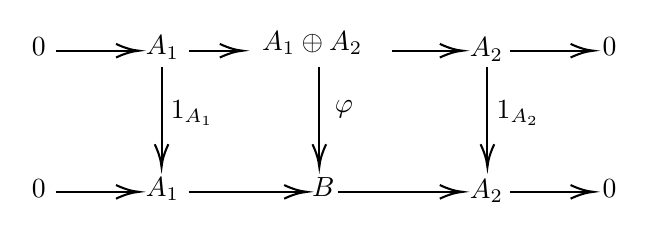
\begin{tikzpicture}[x=0.75pt,y=0.75pt,yscale=-1,xscale=1]
%uncomment if require: \path (0,476); %set diagram left start at 0, and has height of 476

%Straight Lines [id:da22573280049285005] 
\draw    (134,224) -- (172,224) ;
\draw [shift={(174,224)}, rotate = 180] [color={rgb, 255:red, 0; green, 0; blue, 0 }  ][line width=0.75]    (10.93,-3.29) .. controls (6.95,-1.4) and (3.31,-0.3) .. (0,0) .. controls (3.31,0.3) and (6.95,1.4) .. (10.93,3.29)   ;
%Straight Lines [id:da5007083409135236] 
\draw    (198,224) -- (222,224) ;
\draw [shift={(224,224)}, rotate = 180] [color={rgb, 255:red, 0; green, 0; blue, 0 }  ][line width=0.75]    (10.93,-3.29) .. controls (6.95,-1.4) and (3.31,-0.3) .. (0,0) .. controls (3.31,0.3) and (6.95,1.4) .. (10.93,3.29)   ;
%Straight Lines [id:da49627755138453633] 
\draw    (296,224) -- (328,224) ;
\draw [shift={(330,224)}, rotate = 180] [color={rgb, 255:red, 0; green, 0; blue, 0 }  ][line width=0.75]    (10.93,-3.29) .. controls (6.95,-1.4) and (3.31,-0.3) .. (0,0) .. controls (3.31,0.3) and (6.95,1.4) .. (10.93,3.29)   ;
%Straight Lines [id:da7229825431747845] 
\draw    (353,224) -- (391,224) ;
\draw [shift={(393,224)}, rotate = 180] [color={rgb, 255:red, 0; green, 0; blue, 0 }  ][line width=0.75]    (10.93,-3.29) .. controls (6.95,-1.4) and (3.31,-0.3) .. (0,0) .. controls (3.31,0.3) and (6.95,1.4) .. (10.93,3.29)   ;
%Straight Lines [id:da9219190287457819] 
\draw    (185,232) -- (185,278) ;
\draw [shift={(185,280)}, rotate = 270] [color={rgb, 255:red, 0; green, 0; blue, 0 }  ][line width=0.75]    (10.93,-3.29) .. controls (6.95,-1.4) and (3.31,-0.3) .. (0,0) .. controls (3.31,0.3) and (6.95,1.4) .. (10.93,3.29)   ;
%Straight Lines [id:da4241610695219813] 
\draw    (261,232) -- (261,278) ;
\draw [shift={(261,280)}, rotate = 270] [color={rgb, 255:red, 0; green, 0; blue, 0 }  ][line width=0.75]    (10.93,-3.29) .. controls (6.95,-1.4) and (3.31,-0.3) .. (0,0) .. controls (3.31,0.3) and (6.95,1.4) .. (10.93,3.29)   ;
%Straight Lines [id:da5742073517286415] 
\draw    (342,232) -- (342,278) ;
\draw [shift={(342,280)}, rotate = 270] [color={rgb, 255:red, 0; green, 0; blue, 0 }  ][line width=0.75]    (10.93,-3.29) .. controls (6.95,-1.4) and (3.31,-0.3) .. (0,0) .. controls (3.31,0.3) and (6.95,1.4) .. (10.93,3.29)   ;
%Straight Lines [id:da062379905314969175] 
\draw    (134,292) -- (172,292) ;
\draw [shift={(174,292)}, rotate = 180] [color={rgb, 255:red, 0; green, 0; blue, 0 }  ][line width=0.75]    (10.93,-3.29) .. controls (6.95,-1.4) and (3.31,-0.3) .. (0,0) .. controls (3.31,0.3) and (6.95,1.4) .. (10.93,3.29)   ;
%Straight Lines [id:da2958761370037739] 
\draw    (198,292) -- (253,292) ;
\draw [shift={(255,292)}, rotate = 180] [color={rgb, 255:red, 0; green, 0; blue, 0 }  ][line width=0.75]    (10.93,-3.29) .. controls (6.95,-1.4) and (3.31,-0.3) .. (0,0) .. controls (3.31,0.3) and (6.95,1.4) .. (10.93,3.29)   ;
%Straight Lines [id:da3240286217569581] 
\draw    (270,292) -- (328,292) ;
\draw [shift={(330,292)}, rotate = 180] [color={rgb, 255:red, 0; green, 0; blue, 0 }  ][line width=0.75]    (10.93,-3.29) .. controls (6.95,-1.4) and (3.31,-0.3) .. (0,0) .. controls (3.31,0.3) and (6.95,1.4) .. (10.93,3.29)   ;
%Straight Lines [id:da0337697350918047] 
\draw    (353,292) -- (391,292) ;
\draw [shift={(393,292)}, rotate = 180] [color={rgb, 255:red, 0; green, 0; blue, 0 }  ][line width=0.75]    (10.93,-3.29) .. controls (6.95,-1.4) and (3.31,-0.3) .. (0,0) .. controls (3.31,0.3) and (6.95,1.4) .. (10.93,3.29)   ;

% Text Node
\draw (121,216.4) node [anchor=north west][inner sep=0.75pt]    {$0$};
% Text Node
\draw (176,215.4) node [anchor=north west][inner sep=0.75pt]    {$A_{1}$};
% Text Node
\draw (232,213.4) node [anchor=north west][inner sep=0.75pt]    {$A_{1} \oplus A_{2}$};
% Text Node
\draw (332,216.4) node [anchor=north west][inner sep=0.75pt]    {$A_{2}$};
% Text Node
\draw (396,216.4) node [anchor=north west][inner sep=0.75pt]    {$0$};
% Text Node
\draw (188,246.4) node [anchor=north west][inner sep=0.75pt]    {$1_{A_{1}}$};
% Text Node
\draw (267,246.4) node [anchor=north west][inner sep=0.75pt]    {$\varphi $};
% Text Node
\draw (345,246.4) node [anchor=north west][inner sep=0.75pt]    {$1_{A_{2}}$};
% Text Node
\draw (121,284.4) node [anchor=north west][inner sep=0.75pt]    {$0$};
% Text Node
\draw (176,283.4) node [anchor=north west][inner sep=0.75pt]    {$A_{1}$};
% Text Node
\draw (256,283.4) node [anchor=north west][inner sep=0.75pt]    {$B$};
% Text Node
\draw (332,284.4) node [anchor=north west][inner sep=0.75pt]    {$A_{2}$};
% Text Node
\draw (396,284.4) node [anchor=north west][inner sep=0.75pt]    {$0$};


\end{tikzpicture}
\end{center}
is commutative, whence by the Short Five Lemma we have the two short exact sequence are isomorphic.\par
(ii)$\Rightarrow$(iii): Define $\psi:B\to A_1\oplus A_2$ by $b\mapsto(k(b),g(b))$. Observe that the diagram 
\begin{center}


\tikzset{every picture/.style={line width=0.75pt}} %set default line width to 0.75pt        

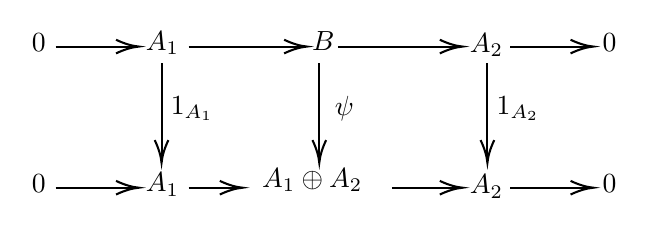
\begin{tikzpicture}[x=0.75pt,y=0.75pt,yscale=-1,xscale=1]
%uncomment if require: \path (0,476); %set diagram left start at 0, and has height of 476

%Straight Lines [id:da22573280049285005] 
\draw    (134,224) -- (172,224) ;
\draw [shift={(174,224)}, rotate = 180] [color={rgb, 255:red, 0; green, 0; blue, 0 }  ][line width=0.75]    (10.93,-3.29) .. controls (6.95,-1.4) and (3.31,-0.3) .. (0,0) .. controls (3.31,0.3) and (6.95,1.4) .. (10.93,3.29)   ;
%Straight Lines [id:da5007083409135236] 
\draw    (198,292) -- (222,292) ;
\draw [shift={(224,292)}, rotate = 180] [color={rgb, 255:red, 0; green, 0; blue, 0 }  ][line width=0.75]    (10.93,-3.29) .. controls (6.95,-1.4) and (3.31,-0.3) .. (0,0) .. controls (3.31,0.3) and (6.95,1.4) .. (10.93,3.29)   ;
%Straight Lines [id:da49627755138453633] 
\draw    (296,292) -- (328,292) ;
\draw [shift={(330,292)}, rotate = 180] [color={rgb, 255:red, 0; green, 0; blue, 0 }  ][line width=0.75]    (10.93,-3.29) .. controls (6.95,-1.4) and (3.31,-0.3) .. (0,0) .. controls (3.31,0.3) and (6.95,1.4) .. (10.93,3.29)   ;
%Straight Lines [id:da7229825431747845] 
\draw    (353,224) -- (391,224) ;
\draw [shift={(393,224)}, rotate = 180] [color={rgb, 255:red, 0; green, 0; blue, 0 }  ][line width=0.75]    (10.93,-3.29) .. controls (6.95,-1.4) and (3.31,-0.3) .. (0,0) .. controls (3.31,0.3) and (6.95,1.4) .. (10.93,3.29)   ;
%Straight Lines [id:da9219190287457819] 
\draw    (185,232) -- (185,278) ;
\draw [shift={(185,280)}, rotate = 270] [color={rgb, 255:red, 0; green, 0; blue, 0 }  ][line width=0.75]    (10.93,-3.29) .. controls (6.95,-1.4) and (3.31,-0.3) .. (0,0) .. controls (3.31,0.3) and (6.95,1.4) .. (10.93,3.29)   ;
%Straight Lines [id:da4241610695219813] 
\draw    (261,232) -- (261,278) ;
\draw [shift={(261,280)}, rotate = 270] [color={rgb, 255:red, 0; green, 0; blue, 0 }  ][line width=0.75]    (10.93,-3.29) .. controls (6.95,-1.4) and (3.31,-0.3) .. (0,0) .. controls (3.31,0.3) and (6.95,1.4) .. (10.93,3.29)   ;
%Straight Lines [id:da5742073517286415] 
\draw    (342,232) -- (342,278) ;
\draw [shift={(342,280)}, rotate = 270] [color={rgb, 255:red, 0; green, 0; blue, 0 }  ][line width=0.75]    (10.93,-3.29) .. controls (6.95,-1.4) and (3.31,-0.3) .. (0,0) .. controls (3.31,0.3) and (6.95,1.4) .. (10.93,3.29)   ;
%Straight Lines [id:da062379905314969175] 
\draw    (134,292) -- (172,292) ;
\draw [shift={(174,292)}, rotate = 180] [color={rgb, 255:red, 0; green, 0; blue, 0 }  ][line width=0.75]    (10.93,-3.29) .. controls (6.95,-1.4) and (3.31,-0.3) .. (0,0) .. controls (3.31,0.3) and (6.95,1.4) .. (10.93,3.29)   ;
%Straight Lines [id:da0337697350918047] 
\draw    (353,292) -- (391,292) ;
\draw [shift={(393,292)}, rotate = 180] [color={rgb, 255:red, 0; green, 0; blue, 0 }  ][line width=0.75]    (10.93,-3.29) .. controls (6.95,-1.4) and (3.31,-0.3) .. (0,0) .. controls (3.31,0.3) and (6.95,1.4) .. (10.93,3.29)   ;
%Straight Lines [id:da7190763458830736] 
\draw    (198,224) -- (253,224) ;
\draw [shift={(255,224)}, rotate = 180] [color={rgb, 255:red, 0; green, 0; blue, 0 }  ][line width=0.75]    (10.93,-3.29) .. controls (6.95,-1.4) and (3.31,-0.3) .. (0,0) .. controls (3.31,0.3) and (6.95,1.4) .. (10.93,3.29)   ;
%Straight Lines [id:da8244393699371844] 
\draw    (270,224) -- (328,224) ;
\draw [shift={(330,224)}, rotate = 180] [color={rgb, 255:red, 0; green, 0; blue, 0 }  ][line width=0.75]    (10.93,-3.29) .. controls (6.95,-1.4) and (3.31,-0.3) .. (0,0) .. controls (3.31,0.3) and (6.95,1.4) .. (10.93,3.29)   ;

% Text Node
\draw (121,216.4) node [anchor=north west][inner sep=0.75pt]    {$0$};
% Text Node
\draw (176,215.4) node [anchor=north west][inner sep=0.75pt]    {$A_{1}$};
% Text Node
\draw (232,281.4) node [anchor=north west][inner sep=0.75pt]    {$A_{1} \oplus A_{2}$};
% Text Node
\draw (332,216.4) node [anchor=north west][inner sep=0.75pt]    {$A_{2}$};
% Text Node
\draw (396,216.4) node [anchor=north west][inner sep=0.75pt]    {$0$};
% Text Node
\draw (188,246.4) node [anchor=north west][inner sep=0.75pt]    {$1_{A_{1}}$};
% Text Node
\draw (267,246.4) node [anchor=north west][inner sep=0.75pt]    {$\psi $};
% Text Node
\draw (345,246.4) node [anchor=north west][inner sep=0.75pt]    {$1_{A_{2}}$};
% Text Node
\draw (121,284.4) node [anchor=north west][inner sep=0.75pt]    {$0$};
% Text Node
\draw (176,283.4) node [anchor=north west][inner sep=0.75pt]    {$A_{1}$};
% Text Node
\draw (332,284.4) node [anchor=north west][inner sep=0.75pt]    {$A_{2}$};
% Text Node
\draw (396,284.4) node [anchor=north west][inner sep=0.75pt]    {$0$};
% Text Node
\draw (256,215.4) node [anchor=north west][inner sep=0.75pt]    {$B$};


\end{tikzpicture}
\end{center}
is commutative, whence by the Short Five Lemma two short exact sequences are isomorphic.\par
(iii)$\Rightarrow$(i), (ii): Given a commutative diagram with exact rows and $\varphi$ isomorphism as follows: 
\begin{center}


\tikzset{every picture/.style={line width=0.75pt}} %set default line width to 0.75pt        

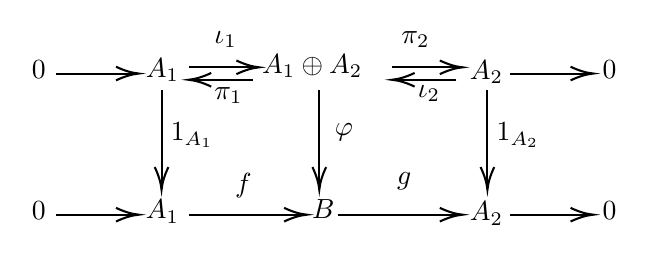
\begin{tikzpicture}[x=0.75pt,y=0.75pt,yscale=-1,xscale=1]
%uncomment if require: \path (0,476); %set diagram left start at 0, and has height of 476

%Straight Lines [id:da22573280049285005] 
\draw    (134,224) -- (172,224) ;
\draw [shift={(174,224)}, rotate = 180] [color={rgb, 255:red, 0; green, 0; blue, 0 }  ][line width=0.75]    (10.93,-3.29) .. controls (6.95,-1.4) and (3.31,-0.3) .. (0,0) .. controls (3.31,0.3) and (6.95,1.4) .. (10.93,3.29)   ;
%Straight Lines [id:da5007083409135236] 
\draw    (198,221) -- (230,221) ;
\draw [shift={(232,221)}, rotate = 180] [color={rgb, 255:red, 0; green, 0; blue, 0 }  ][line width=0.75]    (10.93,-3.29) .. controls (6.95,-1.4) and (3.31,-0.3) .. (0,0) .. controls (3.31,0.3) and (6.95,1.4) .. (10.93,3.29)   ;
%Straight Lines [id:da49627755138453633] 
\draw    (296,221) -- (328,221) ;
\draw [shift={(330,221)}, rotate = 180] [color={rgb, 255:red, 0; green, 0; blue, 0 }  ][line width=0.75]    (10.93,-3.29) .. controls (6.95,-1.4) and (3.31,-0.3) .. (0,0) .. controls (3.31,0.3) and (6.95,1.4) .. (10.93,3.29)   ;
%Straight Lines [id:da7229825431747845] 
\draw    (353,224) -- (391,224) ;
\draw [shift={(393,224)}, rotate = 180] [color={rgb, 255:red, 0; green, 0; blue, 0 }  ][line width=0.75]    (10.93,-3.29) .. controls (6.95,-1.4) and (3.31,-0.3) .. (0,0) .. controls (3.31,0.3) and (6.95,1.4) .. (10.93,3.29)   ;
%Straight Lines [id:da9219190287457819] 
\draw    (185,232) -- (185,278) ;
\draw [shift={(185,280)}, rotate = 270] [color={rgb, 255:red, 0; green, 0; blue, 0 }  ][line width=0.75]    (10.93,-3.29) .. controls (6.95,-1.4) and (3.31,-0.3) .. (0,0) .. controls (3.31,0.3) and (6.95,1.4) .. (10.93,3.29)   ;
%Straight Lines [id:da4241610695219813] 
\draw    (261,232) -- (261,278) ;
\draw [shift={(261,280)}, rotate = 270] [color={rgb, 255:red, 0; green, 0; blue, 0 }  ][line width=0.75]    (10.93,-3.29) .. controls (6.95,-1.4) and (3.31,-0.3) .. (0,0) .. controls (3.31,0.3) and (6.95,1.4) .. (10.93,3.29)   ;
%Straight Lines [id:da5742073517286415] 
\draw    (342,232) -- (342,278) ;
\draw [shift={(342,280)}, rotate = 270] [color={rgb, 255:red, 0; green, 0; blue, 0 }  ][line width=0.75]    (10.93,-3.29) .. controls (6.95,-1.4) and (3.31,-0.3) .. (0,0) .. controls (3.31,0.3) and (6.95,1.4) .. (10.93,3.29)   ;
%Straight Lines [id:da062379905314969175] 
\draw    (134,292) -- (172,292) ;
\draw [shift={(174,292)}, rotate = 180] [color={rgb, 255:red, 0; green, 0; blue, 0 }  ][line width=0.75]    (10.93,-3.29) .. controls (6.95,-1.4) and (3.31,-0.3) .. (0,0) .. controls (3.31,0.3) and (6.95,1.4) .. (10.93,3.29)   ;
%Straight Lines [id:da2958761370037739] 
\draw    (198,292) -- (253,292) ;
\draw [shift={(255,292)}, rotate = 180] [color={rgb, 255:red, 0; green, 0; blue, 0 }  ][line width=0.75]    (10.93,-3.29) .. controls (6.95,-1.4) and (3.31,-0.3) .. (0,0) .. controls (3.31,0.3) and (6.95,1.4) .. (10.93,3.29)   ;
%Straight Lines [id:da3240286217569581] 
\draw    (270,292) -- (328,292) ;
\draw [shift={(330,292)}, rotate = 180] [color={rgb, 255:red, 0; green, 0; blue, 0 }  ][line width=0.75]    (10.93,-3.29) .. controls (6.95,-1.4) and (3.31,-0.3) .. (0,0) .. controls (3.31,0.3) and (6.95,1.4) .. (10.93,3.29)   ;
%Straight Lines [id:da0337697350918047] 
\draw    (353,292) -- (391,292) ;
\draw [shift={(393,292)}, rotate = 180] [color={rgb, 255:red, 0; green, 0; blue, 0 }  ][line width=0.75]    (10.93,-3.29) .. controls (6.95,-1.4) and (3.31,-0.3) .. (0,0) .. controls (3.31,0.3) and (6.95,1.4) .. (10.93,3.29)   ;
%Straight Lines [id:da3278595213426152] 
\draw    (229,227) -- (200,227) ;
\draw [shift={(198,227)}, rotate = 360] [color={rgb, 255:red, 0; green, 0; blue, 0 }  ][line width=0.75]    (10.93,-3.29) .. controls (6.95,-1.4) and (3.31,-0.3) .. (0,0) .. controls (3.31,0.3) and (6.95,1.4) .. (10.93,3.29)   ;
%Straight Lines [id:da9309139657319496] 
\draw    (327,227) -- (298,227) ;
\draw [shift={(296,227)}, rotate = 360] [color={rgb, 255:red, 0; green, 0; blue, 0 }  ][line width=0.75]    (10.93,-3.29) .. controls (6.95,-1.4) and (3.31,-0.3) .. (0,0) .. controls (3.31,0.3) and (6.95,1.4) .. (10.93,3.29)   ;

% Text Node
\draw (121,216.4) node [anchor=north west][inner sep=0.75pt]    {$0$};
% Text Node
\draw (176,215.4) node [anchor=north west][inner sep=0.75pt]    {$A_{1}$};
% Text Node
\draw (232,213.4) node [anchor=north west][inner sep=0.75pt]    {$A_{1} \oplus A_{2}$};
% Text Node
\draw (332,216.4) node [anchor=north west][inner sep=0.75pt]    {$A_{2}$};
% Text Node
\draw (396,216.4) node [anchor=north west][inner sep=0.75pt]    {$0$};
% Text Node
\draw (188,246.4) node [anchor=north west][inner sep=0.75pt]    {$1_{A_{1}}$};
% Text Node
\draw (267,246.4) node [anchor=north west][inner sep=0.75pt]    {$\varphi $};
% Text Node
\draw (345,246.4) node [anchor=north west][inner sep=0.75pt]    {$1_{A_{2}}$};
% Text Node
\draw (121,284.4) node [anchor=north west][inner sep=0.75pt]    {$0$};
% Text Node
\draw (176,283.4) node [anchor=north west][inner sep=0.75pt]    {$A_{1}$};
% Text Node
\draw (256,283.4) node [anchor=north west][inner sep=0.75pt]    {$B$};
% Text Node
\draw (332,284.4) node [anchor=north west][inner sep=0.75pt]    {$A_{2}$};
% Text Node
\draw (396,284.4) node [anchor=north west][inner sep=0.75pt]    {$0$};
% Text Node
\draw (219,270.4) node [anchor=north west][inner sep=0.75pt]    {$f$};
% Text Node
\draw (297,270.4) node [anchor=north west][inner sep=0.75pt]    {$g$};
% Text Node
\draw (209,202.4) node [anchor=north west][inner sep=0.75pt]    {$\iota _{1}$};
% Text Node
\draw (299,202.4) node [anchor=north west][inner sep=0.75pt]    {$\pi _{2}$};
% Text Node
\draw (209,229.4) node [anchor=north west][inner sep=0.75pt]    {$\pi _{1}$};
% Text Node
\draw (307,228.4) node [anchor=north west][inner sep=0.75pt]    {$\iota _{2}$};


\end{tikzpicture}
\end{center}
we define $h:A_2\to B$ to be $\varphi\iota_2$ and $k:B\to A$ to be $\pi_1\varphi^{-1}$, then it is easy to verify that $h$ and $k$ satisfy the conditions.
\end{proof}
\begin{center}
\begin{large}
    \textbf{Exercises for 5.1}
\end{large}
\end{center}
Note that $R$ is a ring.
\begin{problem}\em
If $A$ is an abelian group and $n>0$ an integer such that $na=0$ for all $a\in A$, then $A$ is a unitary $\mathbb{Z}_n$-module, with the action of $\mathbb{Z}_n$ on $A$ given by $\overline{k}a=ka$, there $k\in\mathbb{Z}$ and $k\mapsto\overline{k}\in\mathbb{Z}_n$ under the canonical projection $\mathbb{Z}\to\mathbb{Z}_n$.
\end{problem}
\begin{proof}
Let $a,b\in A$ and $\overline{r},\overline{s}\in\mathbb{Z}_n$, then clearly $(\overline{r})(a+b)=r(a+b)=ra+rb$, $(\overline{r}+\overline{s})a=(r+s)a=ra+sa$ and $(\overline{r}\overline{s})a=(rs)a=r(sa)$, which showed that $A$ is a $\mathbb{Z}_n$-module.
\end{proof}
\begin{problem}\em
Let $f:A\to B$ be an $R$-module homomorphism.\par
(a) $f$ is a monomorphism if and only if for every pair of $R$-module homomorphisms $g,h:D\to A$ such that $fg=fh$, we have $g=h$.\par
(b) $f$ is an epimorphism if and only if for every pair of $R$-module homomorphisms $k,t:B\to C$ such that $kf=tf$, we have $k=t$.
\end{problem}
\begin{proof}
(a) Suppose $f$ is a monomorphism and $fg=fh$. Then for all $x\in D$ we have $fg(x)=fh(x)$, whence $f[g(x)-g(x)]=0$. Therefore $g(x)-h(x)\in\mathrm{Ker}f$. Since $f$ is a monomorphism, we obtain $g(x)-h(x)=0$, whence $g(x)=h(x)$. Conversely, let $D=\mathrm{Ker}f$, $g$ the inclusion map and $h$ the zero map. Then for all $x\in\mathrm{Ker}f$ we have $fg(x)=fh(x)$, whence $fg=fh$. Then by the assumption we conclude that $g=h$, which shows that $\mathrm{Ker}f=0$.\par
(b) Suppose $f$ is an epimorphism and $kf=tf$. Then for all $b\in B$ there exists some $a\in A$ such that $f(a)=b$, and hence $kf(a)=tf(a)$. Since this is true for all $b\in B$, we have $k=f$. Conversely, let $k$ be the canonical epimorphism $B\to B/\mathrm{Im}f$ and $t$ the zero map. Therefore for all $a\in A$ we have $kf(a)=tf(a)=0$, whence $k=t$. This implies $B/\mathrm{Im}f=0$, which is $B=\mathrm{Im}f$ and $f$ an epimorphism.
\end{proof}
\begin{problem}\em
Let $I$ be a left ideal of a ring $R$ and $A$ an $R$-module.\par
(a) If $S$ is a nonempty subset of $A$, then $IS=\left\{\sum_{i=1}^nr_ia_i:n\in\mathbb{N}_+,r_i\in I,a_i\in S\right\}$ is a submodule of $A$. Note that if $S=\{a\}$, then $IS=Ia=\{ra:r\in I\}$.\par
(b) If $I$ is a two-sided ideal, then $A/IA$ is an $R/I$-module with the action of $R/I$ given by $(r+I)(a+IA)=ra+IA$.
\end{problem}
\begin{proof}
(a) Clearly $IS$ is an additive abelian group. Now for all $r\in R$, we have $r\cdot r_ia_i\in IS$ since $I$ is a left ideal of $R$, whence $IS$ is a submodule of $A$.\par
(b) Clearly $A/IA$ is an abelian group. Suppose $r+I$, $s+I\in R/I$ and $a+IA$, $b+IA\in A/IA$, we have $(r+s+I)(a+IA)=(r+s)a+IA=(r+IA)+(s+IA)$, $(r+I)(a+b+IA)=r(a+b)+IA=(ra+IA)+(rb+IA)$ and $((r+I)(s+I))(a+IA)=(r+I)((s+I)(a+IA))$, therefore $A/IA$ is an $R/I$-module with the action of $R/I$ given by $(r+I)(a+IA)=ra+IA$.
\end{proof}
\begin{problem}\em
If $R$ has an identity, then every unitary cyclic $R$-module is isomorphic to an $R$-module of the form $R/J$, where $J$ is a left ideal of $R$.
\end{problem}
\begin{proof}
We define $J=\{x\in A:xa=0\}$. We first show that $J$ is a left ideal of $R$. Suppose $r\in R$, then $rJ\subset J$. Next, define the action of $R$ by multiplication, then $R/J$ is easily seen an $R$-module. Now suppose $A$ is cyclic, i.e., $A=\{ra:r\in R\}$, then define a homomorphism $f:R\to A$ given by $r\mapsto ra$, clearly $f$ is an epimorphism. Therefore by the First Isomorphism Theorem we obtain $A/\mathrm{Ker}f=A/J\cong R$, which finished the proof.
\end{proof}
\begin{problem}\em
If $R$ has an identity, then a nonzero unitary $R$-module $A$ is \textbf{simple} if and only if its submodules are $0$ and $A$.\par
(a) Every simple $R$-module is cyclic.\par
(b) If $A$ is simple every $R$-module endomorphism is either the zero map or an isomorphism.
\end{problem}
\begin{proof}
(a) Suppose $A$ is a simple $R$-module, then for all $a\in A$, we have $ra\in A$ for all $r\in R$, whence $A=Ra$ and it is cyclic.\par
(b) Suppose $f\in\mathrm{End}_RA$, then since $\mathrm{Ker}f$ and $\mathrm{Im}f$ are submodules of $A$, we have $\mathrm{Ker}f=0$ or $\mathrm{Ker}f=A$ (the same is true for $\mathrm{Im}f$). Suppose $x\in R$ and $x\ne 0$. If $x\in\mathrm{Ker}f$, then $\mathrm{Ker}f=A$, whence $f$ is zero map. If $x\notin\mathrm{Ker}f$, then $\mathrm{Ker}f=0$, and hence $f$ is monomorphism. Since $f(x)\ne 0$, it forces $\mathrm{Im}f=A$ and hence $f$ is an isomorphism.
\end{proof}
\begin{problem}\em
A finitely generated $R$-module need not be finitely generated abelian group.
\end{problem}
\begin{proof}
Consider $\mathbb{Q}$. Clearly $\mathbb{Q}$ is a finitely generated $\mathbb{Q}$-module, however, $\mathbb{Q}$ is not a finitely generated abelian group.
\end{proof}
\begin{problem}\em
(a) If $A$ and $B$ are $R$-modules, then the set $\mathrm{Hom}_R(A,B)$ of all $R$-module homomorphisms $A\to B$ is an abelian group with $f+g$ given on $a\in A$ by $(f+g)(a)=f(a)+g(a)\in B$. The identity element is the zero map.\par
(b) $\mathrm{End}_RA=\mathrm{Hom}_R(A,A)$ is a ring with identity, where multiplication is composition of functions. $\mathrm{End}_RA$ is called the \textbf{endomorphism ring} of $A$.\par
(c) $A$ is a left $\mathrm{End}_RA$-module with $fa$ defined to be $f(a)$, $a\in A$, $f\in\mathrm{End}_RA$.
\end{problem}
\begin{proof}
(a) Observe that $(f+g)(x)=f(x)+g(x)=g(x)+f(x)=(g+f)(x)$ for all $x\in A$.\par
(b) By (a) we have $(\mathrm{End}_RA,+)$ is an abelian group. Now we show that $\mathrm{End}_RA$ is a ring. Observe that $(f+g)h=fh+gh$, $h(f+g)=hf+hg$, and $f(gh)=(fg)h$, we have $\mathrm{End}_RA$ is a ring. The identity of $\mathrm{End}_RA$ is $1_{A\to A}$.\par
(c) Suppose $f,g\in\mathrm{End}_RA$ and $a,b\in A$. Then $f(a+b)=f(a)+f(b)$, $(f+g)(a)=f(a)+g(a)$ and $f(g(a))=(fg)(a)$, whence $A$ is an $\mathrm{End}_RA$-module.
\end{proof}
\begin{problem}\em
If $f:A\to A$ is an $R$-module homomorphism such that $ff=f$, then $A=\mathrm{Ker}f\oplus\mathrm{Im}f$.
\end{problem}
\begin{proof}
We consider the short exact sequence: 
$$
0\hookrightarrow \mathrm{Ker}f\longrightarrow A\overset{f}{\longrightarrow}\mathrm{Im}f\longrightarrow 0,
$$
suppose $f(x)=y$, then $ff(x)=f(y)=f(x)=y$, whence $ff\mid_{\mathrm{Im}f}=1_{\mathrm{Im}f}$. Therefore by Theorem 5.12 we have the following diagram 
\begin{center}


\tikzset{every picture/.style={line width=0.75pt}} %set default line width to 0.75pt        

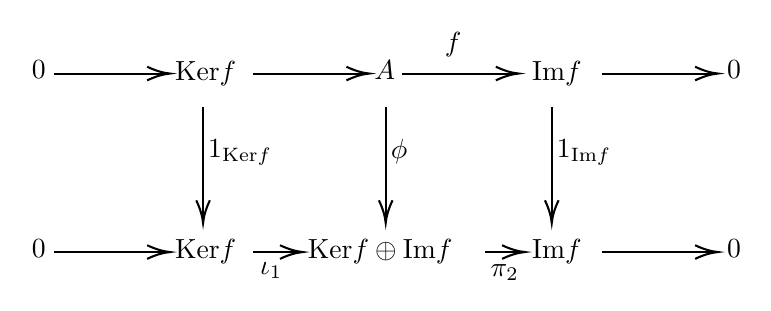
\begin{tikzpicture}[x=0.75pt,y=0.75pt,yscale=-1,xscale=1]
%uncomment if require: \path (0,476); %set diagram left start at 0, and has height of 476

%Straight Lines [id:da11523337004831591] 
\draw    (136,200) -- (190,200) ;
\draw [shift={(192,200)}, rotate = 180] [color={rgb, 255:red, 0; green, 0; blue, 0 }  ][line width=0.75]    (10.93,-3.29) .. controls (6.95,-1.4) and (3.31,-0.3) .. (0,0) .. controls (3.31,0.3) and (6.95,1.4) .. (10.93,3.29)   ;
%Straight Lines [id:da7904190363259922] 
\draw    (232,200) -- (286,200) ;
\draw [shift={(288,200)}, rotate = 180] [color={rgb, 255:red, 0; green, 0; blue, 0 }  ][line width=0.75]    (10.93,-3.29) .. controls (6.95,-1.4) and (3.31,-0.3) .. (0,0) .. controls (3.31,0.3) and (6.95,1.4) .. (10.93,3.29)   ;
%Straight Lines [id:da587990758726602] 
\draw    (304,200) -- (358,200) ;
\draw [shift={(360,200)}, rotate = 180] [color={rgb, 255:red, 0; green, 0; blue, 0 }  ][line width=0.75]    (10.93,-3.29) .. controls (6.95,-1.4) and (3.31,-0.3) .. (0,0) .. controls (3.31,0.3) and (6.95,1.4) .. (10.93,3.29)   ;
%Straight Lines [id:da9885626053073777] 
\draw    (400,200) -- (454,200) ;
\draw [shift={(456,200)}, rotate = 180] [color={rgb, 255:red, 0; green, 0; blue, 0 }  ][line width=0.75]    (10.93,-3.29) .. controls (6.95,-1.4) and (3.31,-0.3) .. (0,0) .. controls (3.31,0.3) and (6.95,1.4) .. (10.93,3.29)   ;
%Straight Lines [id:da3308579976843522] 
\draw    (136,286) -- (190,286) ;
\draw [shift={(192,286)}, rotate = 180] [color={rgb, 255:red, 0; green, 0; blue, 0 }  ][line width=0.75]    (10.93,-3.29) .. controls (6.95,-1.4) and (3.31,-0.3) .. (0,0) .. controls (3.31,0.3) and (6.95,1.4) .. (10.93,3.29)   ;
%Straight Lines [id:da6671524047453168] 
\draw    (232,286) -- (254,286) ;
\draw [shift={(256,286)}, rotate = 180] [color={rgb, 255:red, 0; green, 0; blue, 0 }  ][line width=0.75]    (10.93,-3.29) .. controls (6.95,-1.4) and (3.31,-0.3) .. (0,0) .. controls (3.31,0.3) and (6.95,1.4) .. (10.93,3.29)   ;
%Straight Lines [id:da4339888772828562] 
\draw    (344,286) -- (361,286) ;
\draw [shift={(363,286)}, rotate = 180] [color={rgb, 255:red, 0; green, 0; blue, 0 }  ][line width=0.75]    (10.93,-3.29) .. controls (6.95,-1.4) and (3.31,-0.3) .. (0,0) .. controls (3.31,0.3) and (6.95,1.4) .. (10.93,3.29)   ;
%Straight Lines [id:da021376580311138982] 
\draw    (400,286) -- (454,286) ;
\draw [shift={(456,286)}, rotate = 180] [color={rgb, 255:red, 0; green, 0; blue, 0 }  ][line width=0.75]    (10.93,-3.29) .. controls (6.95,-1.4) and (3.31,-0.3) .. (0,0) .. controls (3.31,0.3) and (6.95,1.4) .. (10.93,3.29)   ;
%Straight Lines [id:da49203458496172336] 
\draw    (208,216) -- (208,270) ;
\draw [shift={(208,272)}, rotate = 270] [color={rgb, 255:red, 0; green, 0; blue, 0 }  ][line width=0.75]    (10.93,-3.29) .. controls (6.95,-1.4) and (3.31,-0.3) .. (0,0) .. controls (3.31,0.3) and (6.95,1.4) .. (10.93,3.29)   ;
%Straight Lines [id:da12466324878794266] 
\draw    (376,216) -- (376,270) ;
\draw [shift={(376,272)}, rotate = 270] [color={rgb, 255:red, 0; green, 0; blue, 0 }  ][line width=0.75]    (10.93,-3.29) .. controls (6.95,-1.4) and (3.31,-0.3) .. (0,0) .. controls (3.31,0.3) and (6.95,1.4) .. (10.93,3.29)   ;
%Straight Lines [id:da19403386152219593] 
\draw    (296,216) -- (296,270) ;
\draw [shift={(296,272)}, rotate = 270] [color={rgb, 255:red, 0; green, 0; blue, 0 }  ][line width=0.75]    (10.93,-3.29) .. controls (6.95,-1.4) and (3.31,-0.3) .. (0,0) .. controls (3.31,0.3) and (6.95,1.4) .. (10.93,3.29)   ;

% Text Node
\draw (124,192.4) node [anchor=north west][inner sep=0.75pt]    {$0$};
% Text Node
\draw (193,192.4) node [anchor=north west][inner sep=0.75pt]    {$\mathrm{Ker} f$};
% Text Node
\draw (289,192.4) node [anchor=north west][inner sep=0.75pt]    {$A$};
% Text Node
\draw (365,192.4) node [anchor=north west][inner sep=0.75pt]    {$\mathrm{Im} f$};
% Text Node
\draw (459,192.4) node [anchor=north west][inner sep=0.75pt]    {$0$};
% Text Node
\draw (124,278.4) node [anchor=north west][inner sep=0.75pt]    {$0$};
% Text Node
\draw (193,278.4) node [anchor=north west][inner sep=0.75pt]    {$\mathrm{Ker} f$};
% Text Node
\draw (257,278.4) node [anchor=north west][inner sep=0.75pt]    {$\mathrm{Ker} f\oplus \mathrm{Im} f$};
% Text Node
\draw (365,278.4) node [anchor=north west][inner sep=0.75pt]    {$\mathrm{Im} f$};
% Text Node
\draw (459,278.4) node [anchor=north west][inner sep=0.75pt]    {$0$};
% Text Node
\draw (323,178.4) node [anchor=north west][inner sep=0.75pt]    {$f$};
% Text Node
\draw (234,289.4) node [anchor=north west][inner sep=0.75pt]    {$\iota _{1}$};
% Text Node
\draw (345,290.4) node [anchor=north west][inner sep=0.75pt]    {$\pi _{2}$};
% Text Node
\draw (297,230.4) node [anchor=north west][inner sep=0.75pt]    {$\phi $};
% Text Node
\draw (377,230.4) node [anchor=north west][inner sep=0.75pt]    {$1_{\mathrm{Im} f}{}$};
% Text Node
\draw (209,230.4) node [anchor=north west][inner sep=0.75pt]    {$1_{\mathrm{Ker} f}$};


\end{tikzpicture}
\end{center}
is commutative, and hence $\phi$ is an isomorphism. Therefore $A\cong\mathrm{Ker}f\oplus\mathrm{Im}f$.
\end{proof}
\begin{problem}\em
Let $A,A_1,\cdots,A_n$ be $R$-modules. Then $A\cong A_1\oplus A_2\oplus\cdots\oplus A_n$ if and only if for each $i=1,2,\cdots,n$ there is an $R$-module homomorphism $\varphi_i:A\to A$ such that $\mathrm{Im}\varphi_i\cong A_i$, $\varphi_i\varphi_j=0$ for $i\ne j$ and $\varphi_1+\varphi_2+\cdots+\varphi_n=1_A$.
\end{problem}
\begin{proof}
Suppose $A\cong A_1\oplus\cdots\oplus A_n$, then let $\varphi_i=\iota_i\circ\pi_i$. Conversely, given $\{\varphi_i\}$, we first show that $\varphi_i\circ\varphi_i=\varphi_i$. Observe that $\varphi_1+\cdots+\varphi_n=1_A$, we have $\varphi_i\circ\varphi_1+\cdots+\varphi_i\circ\varphi_i+\cdots+\varphi_i\circ\varphi_n=\varphi_i$. However $\varphi_i\circ\varphi_j=0$ when $i\ne j$, we have $\varphi_i\circ\varphi_i=\varphi_i$. Now define $\psi_i=\varphi_i\mid_{\mathrm{Im}\varphi_i}$ and apply Theorem 5.9.
\end{proof}
\begin{problem}\em
(a) If $A$ is a module over a commutative ring $R$ and $a\in A$, then $\mathcal{O}_a=\{r\in R:ra=0\}$ is an ideal of $R$. If $\mathcal{O}_a\ne 0$, $a$ is said to be a \textbf{torsion element} of $A$.\par
(b) If $R$ is an integral domain, then the set $T(A)$ of all torsion elements of $A$ is a submodule of $A$.($T(A)$ is called the \textbf{torsion submodule}.)\par
(c) Show that (b) may be false if $R$ is not an integral domain.\par
In (d)-(f) $R$ is an integral domain.\par
(d) If $f:A\to B$ is an $R$-module homomorphism, then $f(T(A))\subset T(B)$, hence the restriction $f_T$ of $f$ to $T(A)$ is an $R$-module homomorphism $T(A)\to T(B)$.\par
(e) If $0\longrightarrow A\overset{f}{\longrightarrow}B\overset{g}{\longrightarrow}C$ is an exact sequence of $R$-modules, then so is $0\longrightarrow T\left( A \right) \overset{f_T}{\longrightarrow}T\left( B \right) \overset{g_T}{\longrightarrow}T(C)$.\par
(f) If $g:B\to C$ is an $R$-module epimorphism, then $g_T:T(B)\to T(C)$ need not be an epimorphism.
\end{problem}
\begin{proof}
(a) Let $r_0\in R$, then for all $ra\in\mathcal{O}_a$, we have $r_0ra=0$, hence $r_0r\in\mathcal{O}_a$. Since $R$ is commutative, we conclude that $\mathcal{O}_a$ is an ideal of $R$.\par
(b) We first show that $T(A)$ is a additive subgroup of $A$. Let $a,b\in T(A)$, then $\mathcal{O}_a$ and $\mathcal{O}_b$ are both nonempty. Let $r_a\in\mathcal{O}_a$ and $r_b\in\mathcal{O}_b$, then $r_ar_b(a+b)=0$, whence $a+b\in T(A)$. Note that $r_ar_b\ne 0$ since $r_a\ne 0$, $r_b\ne 0$, and $R$ is an integral domain. Now suppose $r_0\in R$, then $r_0ra=0$, hence $T(A)$ is a submodule of $A$.\par
(c) Consider the $\mathbb{Z}/12\mathbb{Z}$-module $\mathbb{Z}/12\mathbb{Z}$. Since $\overline{3}\cdot\overline{4}=\overline{2}\cdot\overline{6}=\overline{0}$, we have $\overline{4},\overline{6}\in T(\mathbb{Z}/12\mathbb{Z})$. However $\overline{4}+\overline{6}=\overline{10}\notin T(\mathbb{Z}/12\mathbb{Z})$.\par
(d) Let $a\in T(A)$, then there exists some nonzero $r\in R$ such that $ra=0$. Therefore $f(ra)=rf(a)=0$, whence $f(a)\in T(B)$. Therefore $f(T(A))\subset T(B)$.\par
(e) Since $0\longrightarrow A\overset{f}{\longrightarrow}B\overset{g}{\longrightarrow}C$ is an exact sequence of $R$-modules, then $\mathrm{Im}f=\mathrm{Ker}g$. Now we show that $\mathrm{Im}f_T=\mathrm{Ker}g_T$. Let $b\in\mathrm{Im}f_T$, then $b\in\mathrm{Im}f$ and hence $b\in\mathrm{Ker}g$. Since $b\in T(B)$ we have $g_T(b)=0$, whence $b\in\mathrm{Ker}g_T$. This shows $\mathrm{Im}f_T\subset\mathrm{Ker}g_T$. For the converse inequality, suppose $b\in\mathrm{Ker}g_T$. Then $b\in\mathrm{Ker}g=\mathrm{Im}f$, therefore there exists some $a\in A$ such that $f(a)=b$. Since $b\in T(B)$, there exists some nonzero $r\in R$ such that $rb=0$. Consider $f(ra)=rf(a)=rb=0$, we have $ra\in\mathrm{Ker}f$. However $\mathrm{Ker}f=0$, therefore $a\in T(A)$, and the proof is finished.\par
(f) Consider $\mathbb{Z}$ and $\mathbb{Z}/4\mathbb{Z}$ as $\mathbb{Z}$-modules, define $g:\mathbb{Z}\mapsto\mathbb{Z}/4\mathbb{Z}$ as $n\mapsto n\ \mathrm{mod}4$.
\end{proof}
\begin{problem}\em
Let 
\begin{center}


\tikzset{every picture/.style={line width=0.75pt}} %set default line width to 0.75pt        

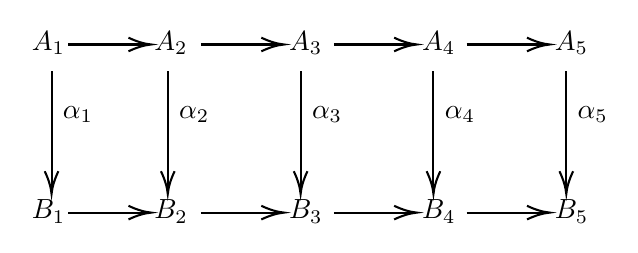
\begin{tikzpicture}[x=0.75pt,y=0.75pt,yscale=-1,xscale=1]
%uncomment if require: \path (0,476); %set diagram left start at 0, and has height of 476

%Straight Lines [id:da2968650742386445] 
\draw    (184,200) -- (222,200) ;
\draw [shift={(224,200)}, rotate = 180] [color={rgb, 255:red, 0; green, 0; blue, 0 }  ][line width=0.75]    (10.93,-3.29) .. controls (6.95,-1.4) and (3.31,-0.3) .. (0,0) .. controls (3.31,0.3) and (6.95,1.4) .. (10.93,3.29)   ;
%Straight Lines [id:da3087931668138173] 
\draw    (248,200) -- (286,200) ;
\draw [shift={(288,200)}, rotate = 180] [color={rgb, 255:red, 0; green, 0; blue, 0 }  ][line width=0.75]    (10.93,-3.29) .. controls (6.95,-1.4) and (3.31,-0.3) .. (0,0) .. controls (3.31,0.3) and (6.95,1.4) .. (10.93,3.29)   ;
%Straight Lines [id:da43900145473204155] 
\draw    (312,200) -- (350,200) ;
\draw [shift={(352,200)}, rotate = 180] [color={rgb, 255:red, 0; green, 0; blue, 0 }  ][line width=0.75]    (10.93,-3.29) .. controls (6.95,-1.4) and (3.31,-0.3) .. (0,0) .. controls (3.31,0.3) and (6.95,1.4) .. (10.93,3.29)   ;
%Straight Lines [id:da7713018854398284] 
\draw    (376,200) -- (414,200) ;
\draw [shift={(416,200)}, rotate = 180] [color={rgb, 255:red, 0; green, 0; blue, 0 }  ][line width=0.75]    (10.93,-3.29) .. controls (6.95,-1.4) and (3.31,-0.3) .. (0,0) .. controls (3.31,0.3) and (6.95,1.4) .. (10.93,3.29)   ;
%Straight Lines [id:da7107268582024568] 
\draw    (184,281) -- (222,281) ;
\draw [shift={(224,281)}, rotate = 180] [color={rgb, 255:red, 0; green, 0; blue, 0 }  ][line width=0.75]    (10.93,-3.29) .. controls (6.95,-1.4) and (3.31,-0.3) .. (0,0) .. controls (3.31,0.3) and (6.95,1.4) .. (10.93,3.29)   ;
%Straight Lines [id:da024645825848374825] 
\draw    (248,281) -- (286,281) ;
\draw [shift={(288,281)}, rotate = 180] [color={rgb, 255:red, 0; green, 0; blue, 0 }  ][line width=0.75]    (10.93,-3.29) .. controls (6.95,-1.4) and (3.31,-0.3) .. (0,0) .. controls (3.31,0.3) and (6.95,1.4) .. (10.93,3.29)   ;
%Straight Lines [id:da01920398666668821] 
\draw    (312,281) -- (350,281) ;
\draw [shift={(352,281)}, rotate = 180] [color={rgb, 255:red, 0; green, 0; blue, 0 }  ][line width=0.75]    (10.93,-3.29) .. controls (6.95,-1.4) and (3.31,-0.3) .. (0,0) .. controls (3.31,0.3) and (6.95,1.4) .. (10.93,3.29)   ;
%Straight Lines [id:da7055791271948879] 
\draw    (376,281) -- (414,281) ;
\draw [shift={(416,281)}, rotate = 180] [color={rgb, 255:red, 0; green, 0; blue, 0 }  ][line width=0.75]    (10.93,-3.29) .. controls (6.95,-1.4) and (3.31,-0.3) .. (0,0) .. controls (3.31,0.3) and (6.95,1.4) .. (10.93,3.29)   ;
%Straight Lines [id:da7896973425174743] 
\draw    (176,213) -- (176,270) ;
\draw [shift={(176,272)}, rotate = 270] [color={rgb, 255:red, 0; green, 0; blue, 0 }  ][line width=0.75]    (10.93,-3.29) .. controls (6.95,-1.4) and (3.31,-0.3) .. (0,0) .. controls (3.31,0.3) and (6.95,1.4) .. (10.93,3.29)   ;
%Straight Lines [id:da6414063846519429] 
\draw    (232,213) -- (232,270) ;
\draw [shift={(232,272)}, rotate = 270] [color={rgb, 255:red, 0; green, 0; blue, 0 }  ][line width=0.75]    (10.93,-3.29) .. controls (6.95,-1.4) and (3.31,-0.3) .. (0,0) .. controls (3.31,0.3) and (6.95,1.4) .. (10.93,3.29)   ;
%Straight Lines [id:da857172487299223] 
\draw    (296,213) -- (296,270) ;
\draw [shift={(296,272)}, rotate = 270] [color={rgb, 255:red, 0; green, 0; blue, 0 }  ][line width=0.75]    (10.93,-3.29) .. controls (6.95,-1.4) and (3.31,-0.3) .. (0,0) .. controls (3.31,0.3) and (6.95,1.4) .. (10.93,3.29)   ;
%Straight Lines [id:da5314329341376476] 
\draw    (360,213) -- (360,270) ;
\draw [shift={(360,272)}, rotate = 270] [color={rgb, 255:red, 0; green, 0; blue, 0 }  ][line width=0.75]    (10.93,-3.29) .. controls (6.95,-1.4) and (3.31,-0.3) .. (0,0) .. controls (3.31,0.3) and (6.95,1.4) .. (10.93,3.29)   ;
%Straight Lines [id:da13029719909082838] 
\draw    (424,213) -- (424,270) ;
\draw [shift={(424,272)}, rotate = 270] [color={rgb, 255:red, 0; green, 0; blue, 0 }  ][line width=0.75]    (10.93,-3.29) .. controls (6.95,-1.4) and (3.31,-0.3) .. (0,0) .. controls (3.31,0.3) and (6.95,1.4) .. (10.93,3.29)   ;

% Text Node
\draw (165,192.4) node [anchor=north west][inner sep=0.75pt]    {$A_{1}$};
% Text Node
\draw (224,192.4) node [anchor=north west][inner sep=0.75pt]    {$A_{2}$};
% Text Node
\draw (289,192.4) node [anchor=north west][inner sep=0.75pt]    {$A_{3}$};
% Text Node
\draw (353,192.4) node [anchor=north west][inner sep=0.75pt]    {$A_{4}$};
% Text Node
\draw (417,192.4) node [anchor=north west][inner sep=0.75pt]    {$A_{5}$};
% Text Node
\draw (165,273.4) node [anchor=north west][inner sep=0.75pt]    {$B_{1}$};
% Text Node
\draw (224,273.4) node [anchor=north west][inner sep=0.75pt]    {$B_{2}$};
% Text Node
\draw (289,273.4) node [anchor=north west][inner sep=0.75pt]    {$B_{3}$};
% Text Node
\draw (353,273.4) node [anchor=north west][inner sep=0.75pt]    {$B_{4}$};
% Text Node
\draw (417,273.4) node [anchor=north west][inner sep=0.75pt]    {$B_{5}$};
% Text Node
\draw (180,228.4) node [anchor=north west][inner sep=0.75pt]    {$\alpha _{1}$};
% Text Node
\draw (236,228.4) node [anchor=north west][inner sep=0.75pt]    {$\alpha _{2}$};
% Text Node
\draw (300,228.4) node [anchor=north west][inner sep=0.75pt]    {$\alpha _{3}$};
% Text Node
\draw (364,228.4) node [anchor=north west][inner sep=0.75pt]    {$\alpha _{4}$};
% Text Node
\draw (428,228.4) node [anchor=north west][inner sep=0.75pt]    {$\alpha _{5}$};


\end{tikzpicture}
\end{center}
be a commutative diagram of $R$-modules and $R$-module homomorphisms, with exact rows. Prove that \par
(a) $\alpha_1$ an epimorphism and $\alpha_2,\alpha_4$ monomorphisms implies $\alpha_3$ monomorphism.\par
(b) $\alpha_5$ an monomorphism and $\alpha_2,\alpha_4$ epimorphisms implies $\alpha_3$ epimorphism.
\end{problem}
\begin{proof}
We only show (a), and (b) may be proved in an analogous way. Suppose $\alpha_3(a_3)=0$, we now show that $a_3=0$. By the commutativity of the diagram we have 
$$
g_3\circ \alpha _3\left( a_3 \right) =\alpha _4\circ f_3\left( a_3 \right) \Rightarrow \alpha _3\in \mathrm{Ker}f_3=\mathrm{Im}f_2,
$$
therefore there exists some $a_2\in A_2$ such that $f_2(a_2)=0$. Again we have 
$$
\alpha _3\circ f_2\left( a_2 \right) =g_2\circ \alpha _2\left( a_2 \right) \Rightarrow \alpha _2\left( a_2 \right) \in \mathrm{Ker}g_2=\mathrm{Im}g_1,
$$
suppose $\alpha_2(a_2)=b_2$, there exists some $b_1\in B_1$ such that $g_1(b_1)=b_2$. Since $\alpha_1$ is an epimorphism, suppose $\alpha_1(a_1)=b_2$. Now that 
$$
g_2\circ g_1\circ \alpha _1\left( a_1 \right) =\alpha _3\circ f_2\circ f_1\left( a_1 \right) \Rightarrow a_1\in \mathrm{Ker}\alpha _2=0,
$$
whence $a_1=0$. Therefore $a_3=0$, and the prove is finished.
\end{proof}
\begin{problem}\em
(a) If $0\longrightarrow A\longrightarrow B\overset{f}{\longrightarrow}C\longrightarrow 0$ and $0\longrightarrow C\overset{g}{\longrightarrow}D\longrightarrow E\longrightarrow 0$ are short exact sequences of modules, then the sequence $0\longrightarrow A\longrightarrow B\overset{g\circ f}{\longrightarrow}D\longrightarrow E\longrightarrow 0$ is exact.\par
(b) Show that every exact sequence may be obtained by splicing together suitable short exact sequences as in (a).
\end{problem}
\begin{proof}
Suppose $\alpha:A\to B$ and $\beta:D\to E$, then by the exactness we have $\mathrm{Im}\alpha=\mathrm{Ker}f$ and $\mathrm{Im}g=\mathrm{Ker}\beta$. It suffices to show $\mathrm{Im}\alpha =\mathrm{Ker}g\circ f,\hspace{0.5cm}\mathrm{Im}g\circ f=\beta $. We first show $\mathrm{Ker}f=\mathrm{Ker}g\circ f$. Clearly $\mathrm{Ker}f\subset\mathrm{Ker}g\circ f$. Conversely, suppose $g\circ f(x)=0$, then $f(x)\in\mathrm{Ker}g$, whence $f(x)=0$. This implies $x\in\mathrm{Ker}f$. Since $\mathrm{Im}\alpha=\mathrm{Ker}f$, this shows that the sequence exact at $B$. Next we show that $\mathrm{Im}g\circ f=\mathrm{Ker}\beta$. Clearly $\mathrm{Im}g\circ f\subset\mathrm{Im}g$. However $\mathrm{Im}f=\mathrm{Ker}C=C$ implies that $f$ is an epimorphism, therefore $\mathrm{Im}g\circ f=\mathrm{Ker}\beta$, and the sequence is exact at $D$. An analogous argument may be made to show that (b) is true.
\end{proof}
\begin{problem}\em
If $f:A\to B$ and $g:B\to A$ are $R$-module homomorphisms such that $gf=1_A$, then $B=\mathrm{Im}f\oplus\mathrm{Ker}g$.
\end{problem}
\begin{proof}
Clearly the exact sequence $0\longrightarrow A\overset{f}{\longrightarrow}B\overset{g}{\longrightarrow}A\longrightarrow 0$ split, therefore it is equivalent to the sequence $0\longrightarrow A\overset{f}{\longrightarrow}\mathrm{Im}f\oplus \mathrm{Ker}g\overset{g}{\longrightarrow}A\longrightarrow 0$. In particular, $B\cong\mathrm{Im}f\oplus\mathrm{Ker}g$.
\end{proof}
\begin{problem}\em
Let $R$ be a ring and $R^{\mathrm{op}}$ is its opposite ring. If $A$ is a left [resp. right] $R$-module, then $A$ is a right [resp. left] $R^{\mathrm{op}}$-module such that $ra=ar$ for all $a\in A$, $r\in R$ and $r\in R^{\mathrm{op}}$.
\end{problem}
\begin{proof}
It suffices to verify the multiplication condition. Indeed, we observe that 
$$
a\left( r\circ s \right) =a\left( sr \right) =\left( as \right) r=r\circ \left( as \right) =\left( ar \right) \circ s,
$$
this finished the proof.
\end{proof}
\begin{problem}\em
(a) If $R$ has an identity and $A$ is an $R$-module, then there are submodules $B$ and $C$ of $A$ such that $B$ is unitary, $RC=0$ and $A=B\oplus C$.\par
(b) Let $A_1$ be another $R$-module, with $A_1=B_1\oplus C_1$ ($B_1$ binary, $RC_1=0$). If $f:A\to A_1$ is an $R$-module homomorphism then $f(B)\subset B_1$ and $f(C)\subset C_1$.\par
(c) If the map $f$ in (b) is an epimorphism [resp. isomorphism], then so are $f\mid_B$ and $f\mid_C$.
\end{problem}
\begin{proof}
(a) We define $B=\{1_Ra:a\in A\}$ and $C=\{a\in A:1_Ra=0\}$, then $B$ and $C$ are easily verified to be submodules of $A$ and $B$ unitary, $RC=0$. Note that for all $a\in A$, we have $a-1_Ra\in C$ and $B\cap C=0$, therefore $A=B\oplus C$.\par
(b) Suppose $f(B)\not\subset B_1$, then there exists some $b\in B$ such that $f(b)\in C$. Say $f(b)\ne 0$ or otherwise $f(b)\in B$. Then $f(1_Rb)=1_Rf(b)$. However $RC_1=0$, we obtain $f(b)=0$, a contradiction! Similarly we have $f(C)\subset C_1$.\par
(c) Suppose $(b_1,0)\in B_1\oplus C_1$. Since $f$ is an epimorphism and $f(B)\subset B_1$, there exists some $(b,0)\in B\oplus C$ such that $(b,0)\mapsto (b_1,0)$, therefore $f\mid_B$ is an epimorphism. Similarly we may show that $f\mid_C$ is an epimorphism, and the condition that $f$ is an isomorphism.
\end{proof}
\begin{problem}\em
Let $R$ be a ring without identity. Embed $R$ in a ring $S$ with identity and characteristic zero as in the proof of Theorem 4.10. Identity $R$ with its image in $S$.\par
(a) Show that every element of $S$ may be uniquely expressed in the form $r1_S+n1_S$, $r\in R, n\in\mathbb{Z}$.\par
(b) If $A$ is an $R$-module and $a\in A$, show that there is a unique $R$-module homomorphism $f:S\to A$ such that $f(1_S)=a$.
\end{problem}
\begin{proof}
(a) We use the notation in Theorem 4.10. Note that $1_S=(0,1)$, therefore for all $(r,n)\in S$, we have $(r,n)=(r,0)(0,1)+(0,n)(0,1)=r1_S+n1_S$.\par
(b) Let $f(r1_S+n1_S)=ra+na$, then it is a routine to check that $f$ satisfy the condition.
\end{proof}
\subsection{Free Modules and Vector Spaces}
In this section we will study the free objects in the category of modules over a ring. We first give some terminologies.\par
A subset $X$ of an $R$-module $A$ is said to be \textbf{linearly independent} provided that for distinct $x_1,\cdots,x_n\in X$ and $r_i\in R$, we have $r_1x_1+r_2x_2+\cdots+r_nx_n=0$ implies $r_i=0$ for every $i$. A set that is not linearly independent is said to be \textbf{linear dependent}. If $A$ is generated as an $R$-module by a set $Y$, then we say that $Y$ \textbf{spans} $A$. If $R$ has an identity and $A$ is unitary, $Y$ spans $A$ if and only if every element of $A$ may be written as a linear combination $r_1y_1+r_2y_2+\cdots+r_ny_n$, where $r_i\in R$ and $y_i\in Y$. A linearly independent subset of $A$ that spans $A$ is called a \textbf{basis} of $A$. Observe that the empty set is (vacuously) linearly independent and is a basis of the zero module.
\begin{theorem}
Let $R$ be a ring with identity. Then the following statement on a unitary $R$-module $F$ is equivalent:\par
(a) $F$ has a nonempty basis;\par
(b) $F$ is the internal direct sum of a family of cyclic $R$-modules, each of which is isomorphic as a left $R$-module to $R$;\par
(c) $F$ is an $R$-module isomorphic to a direct sum of copies of the left $R$-module $R$;\par
(d) $F$ is a free object in the category of unitary $R$-modules.
\end{theorem}
\begin{proof}
(a)$\Rightarrow$(b): Let $X$ be the basis of $F$. Let $x\in X$, then consider the homomorphism $r\mapsto rx$, $r\in R$. Clearly it is an epimorphism. If $rx=0$, then by linear independence we have $r=0$, whence $r\mapsto rx$ is a monomorphism, whence isomorphism. Note that for all $r\in R$ there exists some linear combination of elements in $X$, we have $F\cong\bigoplus_{x\in X}Rx\cong\bigoplus_{x\in X}R$.\par
(b)$\Rightarrow$(c): By (b) we have $R\cong\bigoplus_{x\in X}Rx$ and $Rx\cong R$. Therefore $R\cong\bigoplus_{x\in X}R_x$, where $R_x$ are isomorphic copies of $R$.\par
(c)$\Rightarrow$(a): Suppose $R\cong\bigoplus_{x\in X}R_x$. Take $\theta_x=\{r_i\}$, where $r_i=0$ for $i\ne x$ and $r_i=1_R$ for $i=x$. Then it is easy to verify that $\{\theta_x\}$ is a basis of $F$.\par
(a)$\Rightarrow$(d): Suppose $X$ is the basis of $F$, then for all $u\in F$, $u$ can be written in the form of $\sum_{x\in X}xr_x$ since $X$ spans $F$, here $r_x\in R$. Now define $\overline{f}$ by $\sum_{x\in X}xr_x\mapsto\sum_{x\in X}r_xf(x)$. We first show that $\overline{f}$ is well-defined. Suppose $u=\sum_{x\in X}xr_x=\sum_{x\in X}xs_x$, then $\sum_{x\in X}x(r_x-s_x)=0$, by linear independence we have $r_x=s_x$, whence $\overline{f}$ is well-defined. It is easy to verify that $\overline{f}$ is a homomorphism and $\overline{f}\iota=f$. Now suppose there is another $g$ such that $g\iota=f$. Then for all $x\in X$ we have $g(x)=g\iota(x)=f(x)=\overline{f}(x)$, and since $X$ spans $F$, we have $g=\overline{f}$.\par
(d)$\Rightarrow$(c): By (c)$\Rightarrow$(a) we know that there exists a basis $\{\theta_x\}$ of $F$. By (a)$\Rightarrow$(d) we know that $\bigoplus_{x\in\theta_x}R$ is a free object on the category of unitary $R$-modules. By the uniqueness of free objects in a category we finished the proof.
\end{proof}
\begin{note}\em
The statement (d) may be rephrased into the commutative diagram below: 
\begin{center}


\tikzset{every picture/.style={line width=0.75pt}} %set default line width to 0.75pt        

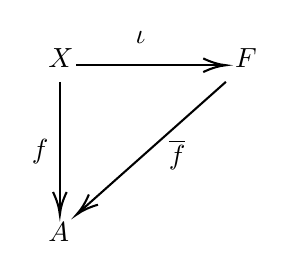
\begin{tikzpicture}[x=0.75pt,y=0.75pt,yscale=-1,xscale=1]
%uncomment if require: \path (0,476); %set diagram left start at 0, and has height of 476

%Straight Lines [id:da31374964360343305] 
\draw    (216,160) -- (286,160) ;
\draw [shift={(288,160)}, rotate = 180] [color={rgb, 255:red, 0; green, 0; blue, 0 }  ][line width=0.75]    (10.93,-3.29) .. controls (6.95,-1.4) and (3.31,-0.3) .. (0,0) .. controls (3.31,0.3) and (6.95,1.4) .. (10.93,3.29)   ;
%Straight Lines [id:da9449415268571746] 
\draw    (208,168) -- (208,230) ;
\draw [shift={(208,232)}, rotate = 270] [color={rgb, 255:red, 0; green, 0; blue, 0 }  ][line width=0.75]    (10.93,-3.29) .. controls (6.95,-1.4) and (3.31,-0.3) .. (0,0) .. controls (3.31,0.3) and (6.95,1.4) .. (10.93,3.29)   ;
%Straight Lines [id:da8254773629074377] 
\draw    (288,168) -- (217.49,230.67) ;
\draw [shift={(216,232)}, rotate = 318.37] [color={rgb, 255:red, 0; green, 0; blue, 0 }  ][line width=0.75]    (10.93,-3.29) .. controls (6.95,-1.4) and (3.31,-0.3) .. (0,0) .. controls (3.31,0.3) and (6.95,1.4) .. (10.93,3.29)   ;

% Text Node
\draw (201,150.4) node [anchor=north west][inner sep=0.75pt]    {$X$};
% Text Node
\draw (291,150.4) node [anchor=north west][inner sep=0.75pt]    {$F$};
% Text Node
\draw (201,234.4) node [anchor=north west][inner sep=0.75pt]    {$A$};
% Text Node
\draw (243,142.4) node [anchor=north west][inner sep=0.75pt]    {$\iota $};
% Text Node
\draw (193,194.4) node [anchor=north west][inner sep=0.75pt]    {$f$};
% Text Node
\draw (259,194.4) node [anchor=north west][inner sep=0.75pt]    {$\overline{f}$};


\end{tikzpicture}
\end{center}
\end{note}
We call an $R$-module $F$ satisfying the conditions in Theorem 5.13 a \textbf{free $R$-module} on the set $X$. Note that $F$ may not be a free object in the category of all $R$-modules. By definition the zero module is the free module on the null set. It is possible to define a free module over the category of all $R$-modules, however such modules will no longer satisfy properties like $F\cong\bigoplus R$. In a few carefully noted instances below, certain results are also valid for these free modules in the category of all $R$-modules. However, unless stated otherwise, the term "free module" will always mean a unitary free module in the sense of Theorem 5.19.
\begin{corollary}
Every (unitary) $R$-module $A$ over a ring $R$ (with identity) is the homomorphic image of a free $R$-module $F$. If $A$ is finitely generated, then $F$ may be chosen to be finitely generated.
\end{corollary}
\begin{proof}
Suppose $X$ is the generators of $A$. Let $F$ be the free object with basis $X$. Then consider the inclusion map $X\to A$, which induces an $R$-module homomorphism $\overline{f}:F\to A$ such that $X\subset\mathrm{Im}\overline{f}$. Since $X$ generates the whole $F$, we have $A=\mathrm{Im}\overline{f}$, and the proof is finished.
\end{proof}
Unlike the condition for free groups, it is not true that the submodules of a free $R$-module is free. For instance, consider a submodule $\{0,2,4\}$ of $\mathbb{Z}_6$, clearly it is not a free $\mathbb{Z}_6$-module.\par
Vector spaces over a division ring $D$ are important, since every vector space over a division ring is indeed a free $D$-module. To prove this, we need the following lemma: 
\begin{lemma}\em
A maximal linearly independent subset $X$ of a vector space $V$ over a division ring $D$ is a basis of $V$.
\end{lemma}
\begin{proof}
Suppose $X$ is a maximal linear independent subset of $V$ and $W$ is spanned by $X$. If $W=V$, then we are done. If not, then there exists some $a\in V$ such that $a\notin W$. Consider $X\cup\{a\}$. If $ra+\sum_{x\in X}xr_x=0$, we show that $r=0$. If not, then $a$ may be represented by a linear combination of elements of $X$, which is a contradiction! Hence $X\cup\{a\}$ is a larger linear independent set of $V$, a contradiction! Therefore $W=V$, and the proof is finished.
\end{proof}
\begin{theorem}
Every vector space $V$ over a division ring $D$ has a basis, whence is a free $D$-module.More generally every linearly independent subset of $V$ is contained in 
a basis of $V$.
\end{theorem}
\begin{proof}
Let $\mathcal{S}$ be the class of all linear independent sets in $V$ and suppose $X$ is any linear independent set in $V$. Clearly $\mathcal{S}$ is nonempty, since the null set $\emptyset$ is contained in $\mathcal{S}$. Define a partial order by inclusion, and therefore there exists a chain $\{C_i:i\in I\}$ in $\mathcal{S}$. Clearly $C=\bigcup_{i\in I} C_i$ is an upper bound of the chain and $C$ is linear independent. By Zorn's lemma there exists a maximal element that contains $X$, and by Lemma 5.2 we conclude that there exists a basis of $V$.
\end{proof}
\begin{theorem}
Let $V$ be a vector space over a division ring $D$, and $X$ is a subset of $V$ that spans $V$, then $X$ contains a basis of $V$.
\end{theorem}
\begin{proof}
Let $\mathcal{S}$ be a partially ordered set of all subsets of $X$ by set inclusion. Then by Zorn's Lemma there exists some maximal element $Y$ that is linear independent in $V$, by Theorem 5.15. Therefore every element in $X$ is a linear combination of elements in $Y$, or otherwise we may add some more elements to $Y$ such that $Y$ is also linear independent, which contradict to the fact that $Y$ is maximal. Therefore since $X$ spans $V$, so is $Y$. Hence $Y$ is a basis of $V$, and the proof is finished.
\end{proof}
We now discuss the cardinality of basis of free modules (vector spaces).
\begin{theorem}
Let $R$ be a ring with identity and $F$ be a free $R$-module with an infinite basis $X$. Then every basis of $F$ has the same cardinality with $X$.
\end{theorem}
\begin{proof}
We first show that every basis of $F$ is infinite. Suppose $Y$ is a finite basis of $R$, then since $X$ is a basis of $F$, then there exists some $\{x_1,\cdots,x_m\}$ that spans all elements of $Y$. Since $X$ has infinitely many elements, take $x\in X\setminus\{x_1,\cdots,x_m\}$. Then since $\{x_1,\cdots,x_m\}$ spans $Y$ and $Y$ is a basis of $F$, we have $x=r_1x_1+\cdots+r_mx_m$ with $r_i\ne 0$ for some $i$. This contradict to the fact that $X$ is linear independent, and hence a contradiction occurs. Therefore $Y$ has infinitely many elements.\par
Suppose $\mathcal{K}(Y)$ denotes all finite subsets of $Y$. Define a map $f:X\to\mathcal{K}(Y)$ given by $x\mapsto r_1y_1+\cdots+r_my_m$. Since $Y$ is a basis of $F$, the map is well-defined. Consider the image $\mathrm{Im}f$ of $f$. Suppose $\mathrm{Im}f$ is finite, then $\bigcup_{\mathcal{S}\in\mathrm{Im}f}\mathcal{S}$ is a finite subset of $Y$ that generates $X$, and hence $F$, a contradiction. Therefore $\mathrm{Im}f$ is infinite.\par
Next we show that $f^{-1}(T)$ is a finite subset of $X$ for every $T\in\mathrm{Im}f\subset\mathcal{K}(Y)$. If $x\in f^{-1}(T)$, then $x$ is contained in the submodule $F_T$ of $F$ generated by $T$, i.e., $f^{-1}(T)\subset F_T$. Since $T$ is finite and each $y\in T$ is a linear combination of a finite number of elements of $X$, there is a finite subset $S$ of $X$ such that $F_T$ is contained in the submodule $F_S$ of $F$ generated by $S$. Since $x\in X$ and $S\subset X$, this contradicts the linear independence of $X$ unless $x\in S$. Therefore $f^{-1}(T)\subset S$, whence $f^{-1}(T)$ is finite.\par
For each $T\in\mathrm{Im}f$, order the elements of $f^{-1}(T)$, say $x_1,\cdots,x_n$, and define an injective map $g_T:f^{-1}(T)\to\mathrm{Im}f\times\mathbb{N}$ by $x_k\mapsto(T,k)$. Verify that the sets $f^{-1}(T)$ form a partition of $X$. It follows that the map $X\to\mathrm{Im}f\times\mathbb{N}$ defined by $x\mapsto g_T(x)$, where $x\in f^{-1}(T)$, is a well-defined injective function, whence $|X|\le|\mathrm{Im}f\times\mathbb{N}|$. Therefore 
$$|X|\le|\mathrm{Im}f\times\mathbb{N}|=|\mathrm{Im}f\cdot\aleph_0|=|\mathrm{Im}f|\le|\mathcal{K}(Y)|=|Y|.$$
Interchanging $X$ and $Y$ in the preceding argument we have $|Y|\le|X|$. Therefore $|X|=|Y|$.
\end{proof}
It is also true that if $V$ is a vector space over a division ring, then any two basis of $V$ has the same cardinality. We skip the proof of this statement.
\begin{definition}
Let $R$ be a ring with identity such that for all free $R$-module $F$ any two basis of $F$ have the same cardinality. Such $R$ is said to have the \textbf{invariant dimension property}, and the cardinality of the basis of $F$ over $R$ is called the \textbf{dimension} or \textbf{rank} of $F$ over $R$.
\end{definition}
As we have proven, any division ring or a commutative ring with identity is a ring with the invariant dimension property. We shall follow the widespread practice of using "dimension" when referring to a vector space and "rank" when referring to a free module. Suppose $D$ is a ring with invariant dimension property and $V$ is a vector space over $D$. Then we denote the dimension of $V$ as $\mathrm{dim}_DV$. We next study the properties of free modules and rings with invariant dimension property.\par
\begin{proposition}
Let $E$ and $F$ are free modules over a ring $R$ that has the invariant of dimension property. Then $E\cong F$ if and only if $E$ and $F$ have the same rank.
\end{proposition}
\begin{proof}
Suppose $X$ is a basis of $E$. Since $E\cong F$, there exists some $\alpha:E\to F$ that is an isomorphism. Since $\alpha(X)$ is a basis of $F$, we have $|X|=|\alpha(X)|=|Y|$ and hence $|E|=|F|$. The converse is Theorem 2.59.
\end{proof}
\begin{lemma}\em
Let $R$ be a ring with identity, $I\ne R$ is an identity of $R$, $F$ is a free $R$-module with basis $X$ and $\pi:F\to F/IF$ the canonical epimorphism. Then $F/IF$ is a free $R/I$-module with basis $\pi(X)$ and $|\pi(X)|=|X|$.
\end{lemma}
\begin{proof}
We first show that $\pi(X)$ generates the whole $F/IF$. Suppose $u+IF\in F/IF$, then $u\in F$ and $u=\sum_ir_ix_i$, where $r_i\in R$ and $x_i\in X$. Therefore 
$$
u+IF=\sum_i{r_ix_i}+IF=\sum_i{\left( r_ix_i+IF \right)}=\sum_i{\left( r_i+I \right) \left( x_i+IF \right)}=\sum_i{\left( r_i+I \right) \pi \left( x_i \right)},
$$
whence $\pi(X)$ spans the whole $F/IF$. Now we show that $\pi(X)$ is a basis of $F/IF$. Suppose 
$$
0=\sum_i{\left( r_i+I \right) \pi \left( x_i \right)}=\sum_i{r_ix_i}+IF,
$$
then $\sum_ir_ix_i\in IF$, whence $\sum_ir_ix_i=\sum_js_ju_j$, where $s_j\in I$ and $u_j\in F$. Note that every element in $F$ can be written into the linear combination of elements in $X$, therefore 
$$
\sum_i{r_ix_i}=\sum_j{s_ju_j}=\sum_j{s_j\left( \sum_k{r_{jk}x_{jk}} \right)}=\sum_j{\sum_k{s_jr_{jk}x_{jk}}}=\sum_l{c_ly_l},
$$
whence $r_i\in I$, and hence $\pi(X)$ is a basis of $F/IF$. Clearly $\pi$ is bijective, whence $|X|=|\pi(X)|$, and the proof is finished.
\end{proof}
\begin{proposition}
Let $f:R\to S$ be a nonzero epimorphism of rings with identity. If $S$ has the invariant dimension property, then so does $R$.
\end{proposition}
\begin{proof}
Suppose $I=\mathrm{Ker}f$, then $S\cong R/I$. Suppose $F$ is a free $R$-module over $R$ and $X$, $Y$ are bases of $F$. Consider $\pi:F\to F/IF$. By Lemma 5.3 we know that $F/IF$ is a free $R/I$-module, which is $S$-module, with bases $\pi(X)$ and $\pi(Y)$. Since $S$ has the invariant dimension property, we have $|\pi(X)|=|\pi(Y)|$, and hence $X=Y$.
\end{proof}
\begin{corollary}
If $R$ is a ring with identity that has a homomorphic image which is a division ring, then $R$ has the invariant dimension property. In particular, every commutative ring with identity has the invariant dimension property.
\end{corollary}
\begin{proof}
The first statement follows from the fact that vector spaces over a division ring is free and Proposition 5.20. For the second part, observe that a commutative ring with identity preserves a maximal ideal $M$, and $R/M$ is a field.
\end{proof}
We now return to vector spaces over a division ring and investigate the properties of dimension. A vector space $V$ over a division ring $D$ is said to be \textbf{finite dimensional} if $\mathrm{dim}_DV$ is finite.
\begin{theorem}
Let $W$ be a subspace of a vector space $V$ over a division ring $D$.\par
(i) $\mathrm{dim}_DW\le\mathrm{dim}_DV$;\par
(ii) If $\mathrm{dim}_DW=\dim_DV$ and $\mathrm{dim}_DV$ is finite, then $W=V$;\par
(iii) $\mathrm{dim}_DV=\mathrm{dim}_DW+\mathrm{dim}_D(V/W)$.
\end{theorem}
\begin{proof}
(i) Suppose $Y$ is a basis of $W$, then $Y$ is linear independent in $V$, whence if $X$ is a basis of $V$, we have $|Y|\le|X|$, whence $\mathrm{dim}_DW\le\mathrm{dim}_DV$.\par
(ii) Since $|Y|=|X|$, then $Y$ and $X$ spans the same space, whence $W=V$.\par
(iii) We show that $U=\{x+W:x\in X-Y\}$ is a basis of $V/W$. Clearly $U$ is linear independent. Now we show that $U$ spans $V/W$. Let $v\in V$, then $v=\sum_ir_iy_i+\sum_js_jx_j$, whence 
$$
v+W=\sum_j{s_jx_j}+W=\sum_j{s_j\left( x_j+W \right)},
$$
whence $U$ spans $V/W$ and hence a basis of $V/W$. Therefore 
$$
\mathrm{dim}_DV=\left| X \right|=\left| Y \right|+\left| X-Y \right|=\left| Y \right|+\left| U \right|=\mathrm{dim}_DW+\mathrm{dim}_DV/W.
$$
\end{proof}
\begin{corollary}
If $f:V\to V^\prime$ is a linear transformation of vector spaces over a division ring $D$, then there exists a basis $X$ of $V$ such that $X\cap\mathrm{Ker}f$ is a basis of $\mathrm{Ker}f$ and $\{f(x):f(x)\ne 0,x\in X\}$ is a basis of $\mathrm{Im}f$. In particular, $\mathrm{dim}_DV=\mathrm{dim}_D\mathrm{Ker}f+\mathrm{dim}_D\mathrm{Im}f$.
\end{corollary}
\begin{proof}
Let $W$ be $\mathrm{Ker}f$ in Theorem 5.22(iii), then $V/W=V/\mathrm{Ker}f\cong\mathrm{Im}f$, whence 
$$
\mathrm{dim}_DV=\mathrm{dim}_D\mathrm{Ker}f+\mathrm{dim}_D\mathrm{Im}f.
$$
\end{proof}
\begin{corollary}
If $V$ and $W$ are finite dimensional subspaces of a vector space over a division ring $D$, then 
$$
\mathrm{dim}_DV+\mathrm{dim}_DW=\mathrm{dim}_D\left( V\cap W \right) +\mathrm{dim}_D\left( V+W \right) .
$$
\end{corollary}
\begin{proof}
Let $X$ be a basis of $V\cap W$, $Y$ a basis of $V$ that contains $X$, and $Z$ a basis of $W$ that contains $X$, it is easy to show that $X\cup(Y-X)\cup(Z-X)$ is a basis of $V+W$, whence 
$$
\begin{aligned}
\mathrm{dim}_D\left( V+W \right)& =\left| X \right|+\left| Y-X \right|+\left| Z-X \right|
\\
&=\mathrm{dim}_D\left( V\cap W \right) +\left( \mathrm{dim}_DW-\mathrm{dim}_D\left( V\cap W \right) \right) +\left( \mathrm{dim}_D-\mathrm{dim}_D\left( V\cap W \right) \right) 
\\
&=\mathrm{dim}_DW+\mathrm{dim}_D-\mathrm{dim}_D\left( V\cap W \right) .
\end{aligned}
$$
\end{proof}
Recall that if a division ring $R$ is contained in a division ring $S$, then $R$ is a vector space over $S$ with $rs$ the ordinary product in $S$.
\begin{theorem}
Let $R,S,T$ be division rings such that $R\subset S\subset T$. Then $\mathrm{dim}_RT=(\mathrm{dim}_ST)(\mathrm{dim}_RS)$. Furthermore $\mathrm{dim}_RT$ is finite if and only if $\mathrm{dim}_ST$ and $\mathrm{dim}_RS$ are finite.
\end{theorem}
\begin{proof}
Suppose $U$ is the basis of $T$ over $S$, and let $V$ the basis of $S$ over $R$. It suffices to show that $VU=\{vu:v\in V,u\in U\}$ is a basis of $T$ over $R$. We first show that $VU$ spans $T$. Let $u\in T$, then $u=\sum_is_iu_i$ for some $s_i\in S$ and $u_i\in U$. Since $s_i$ can be written in the form of $\sum_jr_{ij}v_{ij}$, we have 
$$
u=\sum_i{s_iu_i}=\sum_i{\left( \sum_j{r_{ij}v_{ij}} \right) u_i}=\sum_i{\sum_j{r_{ij}v_{ij}u_i}},
$$
whence $VU$ spans the whole $T$ over $R$. Now we show that $VU$ is linear independent. Suppose that $\sum_i\sum_jr_{ij}v_ju_i=0$. For each $i$, let $s_i=\sum_jr_{ij}v_j\in S$, then 
$$
0=\sum_i{\sum_j{r_{ij}v_ju_i}}=\sum_i{\left( \sum_j{r_{ij}v_j} \right) u_i}=\sum_i{s_iu_i},
$$
whence $s_i=0$. The linear independence of $U$ over $S$ implies $r_{ij}=0$, and hence $VU$ is linear independent over $R$ and hence a basis.
\end{proof}
\begin{center}
\begin{large}
    \textbf{Exercises for 5.2}
\end{large}
\end{center}
\begin{problem}\em
(a) A set of vectors $\{x_1,\cdots,x_n\}$ in a vector space $V$ over a division ring $R$ is linearly dependent if and only if some $x_k$ is a linear combination of the preceding $x_i$.\par
(b) If $\{x_1,x_2,x_3\}$ is a linearly independent subset of $V$, then the set $\{x_1+x_2,x_2+x_3,x_3+x_1\}$ is linearly independent if and only if $\mathrm{Char}R\ne2$.
\end{problem}
\begin{proof}
(a) Suppose $\{x_1,\cdots,x_n\}$ is linear dependent. Then there exists some $r_i$ ($1\le i\le n$) such that $\sum r_ix_i=0$ with $r_k\ne 0$. Then $x_k=-r_k^{-1}\sum_{i\ne j}r_ix_i$. Conversely, suppose $x_k=\sum_{i\ne k}r_ix_i$, then $\sum r_ix_i=0$ with $r_k=-1\ne 0$, whence $\{x_1,\cdots,x_n\}$ is linearly dependent.\par
(b) Suppose $\mathrm{Char}R=2$. Then we have 
$$
\left( x_1+x_2 \right) +\left( x_2+x_3 \right) +\left( x_3+x_1 \right) =2x_1+2x_2+2x_3=0,
$$
a contradiction! Conversely, if $\mathrm{Char}R\ne 2$, then suppose $r_1x_1+r_2x_2+r_3x_3=0$ with some $r_i\ne 0$. Then take 
$$
\begin{cases}
	k_1=r_1+r_2-r_3,\\
	k_2=r_2+r_3-r_1,\\
	k_3=r_3+r_1-r_2,\\
\end{cases}
$$
we have 
$$
k_1\left( x_1+x_2 \right) +k_2\left( x_2+x_3 \right) +k_3\left( x_3+x_1 \right) =2\left( r_1x_1+r_2x_2+r_3x_3 \right) =0,
$$
whence $\{x_1+x_2,x_2+x_3,x_3+x_1\}$ is linear independent.
\end{proof}
\begin{problem}\em
Let $R$ be a principal ideal domain, $A$ a unitary left $R$-module, and $p\in R$ a prime. Let $pA=\{pa:a\in A\}$ and $A[p]=\{a\in A:pa=0\}$.\par
(a) $R/(p)$ is a field.\par
(b) $pA$ and $A[p]$ are submodules of $A$.\par
(c) $A/pA$ is a vector space over $R/(p)$, with $(r+(p))(a+pA)=ra+pA$.\par
(d) $A[p]$ is a vector space over $R/(p)$, with $(r+(p))a=ra$.
\end{problem}
\begin{proof}
(a) Since $p$ is a prime, we have $(p)$ a prime ideal. Since $R$ is a principal ideal domain we have $(p)$ also a maximal ideal, and hence $R/(p)$ is a field.\par
(b) We first show that $pA$ is a submodule of $A$. Let $pa,pb\in pA$. Then $(pa)(pb)=p(pab)\in pA$ and hence $pA$ is a multiplicative subgroup of $A$. Now let $r\in R$, we have $rpa=pra\in pA$, hence $pA$ is a submodule of $A$. Now we show that $A[p]$ is a submodule of $A$. Let $a,b\in A[p]$, then $pab=0$, hence $ab\in A[p]$ and then $A[p]$ is a multiplicative subgroup of $A$. Then suppose $r\in R$, we have $pra=rpa=0$, hence $ra\in A[p]$ and $A[p]$ is a submodule of $A$.\par
(c) We prove by definition. Let $r+(p),s+(p)\in R/(p)$ and $a+pA,b+pA\in A/pA$. Then we observe that 
$$
\left( r+\left( p \right) \right) \left( a+b+pA \right) =r\left( a+b \right) +pA=\left( ra+pA \right) +\left( rb+pA \right) ,
$$
$$
\left( r+s+\left( p \right) \right) \left( a+pA \right) =\left( r+s \right) a+pA=\left( ra+pA \right) +\left( sa+pA \right) ,
$$
and 
$$
\left( r+\left( p \right) \right) \left( s+\left( p \right) \right) \left( a+pA \right) =\left( r+\left( p \right) \right) \left( sa+pA \right) =rsa+pA,
$$
and the fact that $R/(p)$ is a field, we finished the proof.\par
(d) The proof is similar to (c).
\end{proof}
\begin{problem}\em
Let $\mathbb{R}$ and $\mathbb{C}$ be the fields of real and complex numbers respectively.\par
(a) $\mathrm{dim}_\mathbb{R}\mathbb{C}=2$ and $\mathrm{dim}_\mathbb{R}\mathbb{R}=1$.\par
(b) There is no field $\mathbb{K}$ such that $\mathbb{R}\subset\mathbb{K}\subset\mathbb{C}$.
\end{problem}
(a) We first show that $\mathrm{dim}_\mathbb{R}\mathbb{C}=2$. Note that $\{1,\mathrm{i}\}$ is a basis of $\mathbb{C}$ over $\mathbb{R}$, since for all $z\in\mathbb{C}$ we have $z=a+b\mathrm{i}$. Therefore $\mathrm{dim}_\mathbb{R}\mathbb{C}=2$. The fact that $\mathrm{dim}_\mathbb{R}\mathbb{R}$ is trivial.\par
(b) Suppose there exists some $\mathbb{K}$ such that $\mathbb{R}\subset\mathbb{K}\subset\mathbb{C}$, then we show that $\mathbb{K}=\mathbb{R}$ or $\mathbb{K}=\mathbb{C}$. By Theorem 5.25 we have 
$$
2=\mathrm{dim}_{\mathbb{R}}\mathbb{C} =\left( \mathrm{dim}_{\mathbb{K}}\mathbb{C} \right) \left( \mathrm{dim}_{\mathbb{R}}\mathbb{K} \right) .
$$
Therefore whether $\dim_{\mathbb{K}}\mathbb{C}=1$ or $\dim_{\mathbb{R}}\mathbb{K}=1$, which implies $\mathbb{K}=\mathbb{C}$ or $\mathbb{R}=\mathbb{K}$.
\begin{problem}\em
If $V$ is a finite dimensional vector space and $V^m$ is the vector space $V\oplus V\oplus\cdots\oplus V$ ($m$ summands), then for each $m\ge 1$, $V^m$ is finite dimensional and $\mathrm{dim}V^m=m\mathrm{dim}V$.
\end{problem}
\begin{proof}
Suppose $\mathrm{dim}V=n$ and $\{\xi_1,\xi_2,\cdots,\xi_n\}$ is a basis of $V$. Then consider $\{\xi_ie_j\}_{1\le i\le n,1\le j\le m}$, where $e_j=(0,\cdots,0,1,0,\cdots,0)$ with $1$ at the $j$th position. Then it is easy to verify that $\{\xi_ie_j\}$ is a basis of $V^m$ and hence $\mathrm{dim}B^m=m\mathrm{dim}V$.
\end{proof}
\begin{problem}\em
If $F_1$ and $F_2$ are free modules over a ring $R$ with the invariant dimension property, then $\mathrm{rank}(F_1\oplus F_2)=\mathrm{rank}F_1+\mathrm{rank}F_2$.
\end{problem}
\begin{proof}
Suppose $\mathrm{rank}F_i=\infty$ for some $i=1,2$. Then since $R$ has the invariant dimension property, we have $\mathrm{rank}(F_1\oplus F_2)=\infty$ and hence $\mathrm{rank}(F_1\oplus F_2)=\mathrm{rank}F_1+\mathrm{rank}F_2$. Now suppose $\mathrm{rank}F_i<\infty$ for all $i=1,2$. Then we may set the basis of $F_1$ to be $\{\xi_1,\xi_2,\cdots,\xi_n\}$ and the basis of $F_2$ to be $\{\zeta_1,\zeta_2,\cdots,\zeta_m\}$. Therefore 
$$
\left\{ \left( \xi _1,0 \right) ,\left( \xi _2,0 \right) ,\cdots ,\left( \xi _n,0 \right) ,\left( 0,\zeta _1 \right) ,\left( 0,\zeta _2 \right) ,\cdots ,\left( 0,\zeta _m \right) \right\} 
$$
is a basis of $F_1\oplus F_2$, and hence $\mathrm{rank}(F_1\oplus F_2)=\mathrm{rank}F_1+\mathrm{rank}F_2$.
\end{proof}
\begin{problem}\em
Let $R$ be a ring with no zero divisors such that for all $r,s\in R$ there exist $a,b\in R$ not both zero, with $ar+bs=0$.\par
(a) If $R=K\oplus L$ (module direct sum), then $K=0$ or $L=0$.\par
(b) If $R$ has an identity, then $R$ has the invariant dimension property.
\end{problem}
\begin{proof}
(a) Suppose $k\in K$ and $l\in L$. Then there exists some $a,b\in R$ such that $ak+bl=0$. However $K\cap L=\{0\}$ since the sum is direct sum, whence $k=0$ or $l=0$ and the proof is finished.\par
(b) Suppose $R^m\cong R^n$, it suffices to show that $m=n$. Suppose $m>n$ without loss of generality. Therefore $R^m/R^{n-1}\cong R^n/R^{n-1}$, and hence $R\cong R^{n-n+1}\cong R\oplus R^{m-n}$, whence $R=0$ or $R^{m-n}=0$ by (a), a contradiction! Therefore $m=n$ and $R$ has the dimension invariance property.
\end{proof}
\begin{problem}\em
Let $F$ be a free module of infinite rank $\alpha$ over a ring $R$ that has the invariant dimension property. For each canonical $\beta$ such that $0\le\beta\le\alpha$, $F$ has infinitely many proper free submodules of rank $\beta$.
\end{problem}
\begin{proof}
If $\beta<\infty$, then the condition is trivial since $\alpha=\infty$. Otherwise suppose $\alpha=\infty$. Then since $\alpha\le\beta$, there exists some epimorphism from the index set of cardinality $\alpha$ to that of cardinality $\beta$. Let $|I|=\alpha$ and $|J|=\beta$, $\{\xi_j\}_{j\in J}$ is a basis of $F$ and $f$ is the epimorphism. Then $\{\xi_i\}_{i\in f^{-1}(J)}$ is a basis that generated a submodule of $F$. By knowledge of cardinality we know that there are infinitely many such submodules.
\end{proof}
\begin{problem}\em
If $F$ is a free module over a ring with identity such that $F$ has a basis of finite cardinality $n\ge 1$ and another basis of cardinality $n+1$, then $F$ has a basis of cardinality $m$ for every $m\ge n$.
\end{problem}
\begin{proof}
By definition we have $R^n\cong R^{n+1}$. Therefore for all $m\ge n$, we have 
$$
R^m\cong R^n\oplus R^{m-n}\cong R^{n+1}\oplus R^{m-n}\cong R^{m+1}
$$
for all $m\ge n$, whence $R^m\cong R^n$ for all $m\ge n$, and the proof is finished.
\end{proof}
\begin{problem}\em
Let $f:V\to V^\prime$ be a linear transformation of finite dimensional vector spaces $V$ and $V^\prime$ such that $\mathrm{dim}V=\mathrm{dim}V^\prime$. Then the following conditions are equivalent:\par
(i) $f$ is an isomorphism.\par
(ii) $f$ is an epimorphism.\par
(iii) $f$ is a monomorphism.
\end{problem}
\begin{proof}
Let $\mathrm{dim}V=\mathrm{dim}V^\prime=n$. It suffices to show that (ii) and (iii) are equivalent. Suppose $f$ is an epimorphism, then $\mathrm{Im}f=n$, whence $\mathrm{dim}\mathrm{Im}f=n-\mathrm{dim}\mathrm{Ker}f=n$, hence $\mathrm{dim}\mathrm{ker}f=0$, which implies $\mathrm{Ker}f=\{0\}$ and hence $f$ is a monomorphism. Conversely, suppose $f$ is a monomorphism, then $\mathrm{dim}\mathrm{Ker}f=0$ and hence $\mathrm{dim}\mathrm{Im}f=n$, which implies $\mathrm{Im}f=V6\prime$ and hence an epimorphism.
\end{proof}
\subsection{Projective and Injective Modules}
Every free module is projective and arbitrary projective modules (which need not to be free) have some of the same properties as free modules. Projective modules are especially useful in a categorical setting since they are defined solely in terms of modules and homomorphisms. Injectivity, which is also studied here, is the dual notion to projectivity.\par
We first give the definition of a projective module.
\begin{definition}
A module $P$ over a ring $R$ is said to be \textbf{projective} if given any diagram of $R$-module homomorphisms 
\begin{center}


\tikzset{every picture/.style={line width=0.75pt}} %set default line width to 0.75pt        

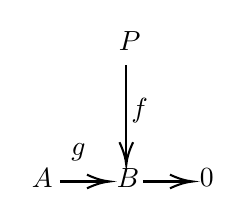
\begin{tikzpicture}[x=0.75pt,y=0.75pt,yscale=-1,xscale=1]
%uncomment if require: \path (0,476); %set diagram left start at 0, and has height of 476

%Straight Lines [id:da9756784236125315] 
\draw    (288,160) -- (288,206) ;
\draw [shift={(288,208)}, rotate = 270] [color={rgb, 255:red, 0; green, 0; blue, 0 }  ][line width=0.75]    (10.93,-3.29) .. controls (6.95,-1.4) and (3.31,-0.3) .. (0,0) .. controls (3.31,0.3) and (6.95,1.4) .. (10.93,3.29)   ;
%Straight Lines [id:da3791632771502693] 
\draw    (256,216) -- (278,216) ;
\draw [shift={(280,216)}, rotate = 180] [color={rgb, 255:red, 0; green, 0; blue, 0 }  ][line width=0.75]    (10.93,-3.29) .. controls (6.95,-1.4) and (3.31,-0.3) .. (0,0) .. controls (3.31,0.3) and (6.95,1.4) .. (10.93,3.29)   ;
%Straight Lines [id:da48034704105691794] 
\draw    (296,216) -- (318,216) ;
\draw [shift={(320,216)}, rotate = 180] [color={rgb, 255:red, 0; green, 0; blue, 0 }  ][line width=0.75]    (10.93,-3.29) .. controls (6.95,-1.4) and (3.31,-0.3) .. (0,0) .. controls (3.31,0.3) and (6.95,1.4) .. (10.93,3.29)   ;

% Text Node
\draw (283,142.4) node [anchor=north west][inner sep=0.75pt]    {$P$};
% Text Node
\draw (241,208.4) node [anchor=north west][inner sep=0.75pt]    {$A$};
% Text Node
\draw (282,208.4) node [anchor=north west][inner sep=0.75pt]    {$B$};
% Text Node
\draw (322,208.4) node [anchor=north west][inner sep=0.75pt]    {$0$};
% Text Node
\draw (289,174.4) node [anchor=north west][inner sep=0.75pt]    {$f$};
% Text Node
\draw (260,196.4) node [anchor=north west][inner sep=0.75pt]    {$g$};


\end{tikzpicture}
\end{center}
with the bottom row exact, i.e. $g$ is an epimorphism, there exists an $R$-module homomorphism $h:P\to A$ such that the diagram 
\begin{center}


\tikzset{every picture/.style={line width=0.75pt}} %set default line width to 0.75pt        

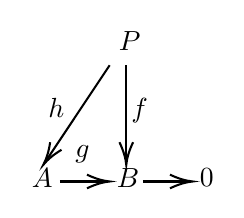
\begin{tikzpicture}[x=0.75pt,y=0.75pt,yscale=-1,xscale=1]
%uncomment if require: \path (0,476); %set diagram left start at 0, and has height of 476

%Straight Lines [id:da9756784236125315] 
\draw    (288,160) -- (288,206) ;
\draw [shift={(288,208)}, rotate = 270] [color={rgb, 255:red, 0; green, 0; blue, 0 }  ][line width=0.75]    (10.93,-3.29) .. controls (6.95,-1.4) and (3.31,-0.3) .. (0,0) .. controls (3.31,0.3) and (6.95,1.4) .. (10.93,3.29)   ;
%Straight Lines [id:da3791632771502693] 
\draw    (256,216) -- (278,216) ;
\draw [shift={(280,216)}, rotate = 180] [color={rgb, 255:red, 0; green, 0; blue, 0 }  ][line width=0.75]    (10.93,-3.29) .. controls (6.95,-1.4) and (3.31,-0.3) .. (0,0) .. controls (3.31,0.3) and (6.95,1.4) .. (10.93,3.29)   ;
%Straight Lines [id:da48034704105691794] 
\draw    (296,216) -- (318,216) ;
\draw [shift={(320,216)}, rotate = 180] [color={rgb, 255:red, 0; green, 0; blue, 0 }  ][line width=0.75]    (10.93,-3.29) .. controls (6.95,-1.4) and (3.31,-0.3) .. (0,0) .. controls (3.31,0.3) and (6.95,1.4) .. (10.93,3.29)   ;
%Straight Lines [id:da36787478006497043] 
\draw    (280,160) -- (249.11,206.34) ;
\draw [shift={(248,208)}, rotate = 303.69] [color={rgb, 255:red, 0; green, 0; blue, 0 }  ][line width=0.75]    (10.93,-3.29) .. controls (6.95,-1.4) and (3.31,-0.3) .. (0,0) .. controls (3.31,0.3) and (6.95,1.4) .. (10.93,3.29)   ;

% Text Node
\draw (283,142.4) node [anchor=north west][inner sep=0.75pt]    {$P$};
% Text Node
\draw (241,208.4) node [anchor=north west][inner sep=0.75pt]    {$A$};
% Text Node
\draw (282,208.4) node [anchor=north west][inner sep=0.75pt]    {$B$};
% Text Node
\draw (322,208.4) node [anchor=north west][inner sep=0.75pt]    {$0$};
% Text Node
\draw (289,174.4) node [anchor=north west][inner sep=0.75pt]    {$f$};
% Text Node
\draw (262,197.4) node [anchor=north west][inner sep=0.75pt]    {$g$};
% Text Node
\draw (249,174.4) node [anchor=north west][inner sep=0.75pt]    {$h$};


\end{tikzpicture}
\end{center}
is commutative, i.e. $gh=f$.
\end{definition}
Our first theorem gives many examples of projective modules. 
\begin{theorem}
Every free module $F$ over a ring $R$ with identity is a projective module.
\end{theorem}
\begin{proof}
We may first assume that modules $A$ and $B$ are unitary. Otherwise by Exercise 5.15 we may decompose $A=A_1\oplus A_2$ and $B=B_1\oplus B_2$, where $A_1$ and $B_1$ are unitary and $RA_2=RB_2=0$. Note that $f(P)\subset B_1$ and $g\mid_{A_1}$ is an epimorphism, whence we may consider the following diagram instead: 
\begin{center}


\tikzset{every picture/.style={line width=0.75pt}} %set default line width to 0.75pt        

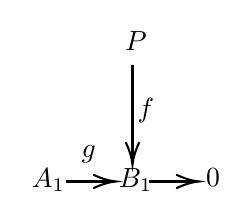
\begin{tikzpicture}[x=0.75pt,y=0.75pt,yscale=-1,xscale=1]
%uncomment if require: \path (0,476); %set diagram left start at 0, and has height of 476

%Straight Lines [id:da9756784236125315] 
\draw    (288,160) -- (288,206) ;
\draw [shift={(288,208)}, rotate = 270] [color={rgb, 255:red, 0; green, 0; blue, 0 }  ][line width=0.75]    (10.93,-3.29) .. controls (6.95,-1.4) and (3.31,-0.3) .. (0,0) .. controls (3.31,0.3) and (6.95,1.4) .. (10.93,3.29)   ;
%Straight Lines [id:da3791632771502693] 
\draw    (256,216) -- (278,216) ;
\draw [shift={(280,216)}, rotate = 180] [color={rgb, 255:red, 0; green, 0; blue, 0 }  ][line width=0.75]    (10.93,-3.29) .. controls (6.95,-1.4) and (3.31,-0.3) .. (0,0) .. controls (3.31,0.3) and (6.95,1.4) .. (10.93,3.29)   ;
%Straight Lines [id:da48034704105691794] 
\draw    (296,216) -- (318,216) ;
\draw [shift={(320,216)}, rotate = 180] [color={rgb, 255:red, 0; green, 0; blue, 0 }  ][line width=0.75]    (10.93,-3.29) .. controls (6.95,-1.4) and (3.31,-0.3) .. (0,0) .. controls (3.31,0.3) and (6.95,1.4) .. (10.93,3.29)   ;

% Text Node
\draw (283,142.4) node [anchor=north west][inner sep=0.75pt]    {$P$};
% Text Node
\draw (238,208.4) node [anchor=north west][inner sep=0.75pt]    {$A_{1}$};
% Text Node
\draw (280,208.4) node [anchor=north west][inner sep=0.75pt]    {$B_{1}$};
% Text Node
\draw (322,208.4) node [anchor=north west][inner sep=0.75pt]    {$0$};
% Text Node
\draw (289,174.4) node [anchor=north west][inner sep=0.75pt]    {$f$};
% Text Node
\draw (262,197.4) node [anchor=north west][inner sep=0.75pt]    {$g$};


\end{tikzpicture}
\end{center}
Now suppose $F$ is a free $R$-module and $A$ and $B$ are unitary. Therefore $F$ is spanned by a basis $X$. Suppose $\iota:X\to F$ is the canonical injection. Since $g$ is an epimorphism, there exists some $a_x\in A$ such that $g(a_x)=f(\iota(x))$. Define $h:x\mapsto a_x$. Since $h$ is determined by elements of $X$, we finished our proof.
\end{proof}
\begin{corollary}
Every module $A$ over a ring $R$ is the homomorphic image of a projective $R$-module.
\end{corollary}
\begin{proof}
By Corollary 5.14 we know that every module $A$ over a ring $R$ is the homomorphic image of a free module. Apply Theorem 5.27 we know that every free module over a ring $R$ is projective, and the proof is finished.
\end{proof}
\begin{theorem}
Let $R$ be a ring. The following conditions on an $R$-module $P$ are equivalent.\par
(a) $P$ is projective;\par
(b) every short exact sequence $0\longrightarrow A\overset{f}{\longrightarrow}B\overset{g}{\longrightarrow}P\longrightarrow 0$ is split exact;\par
(c) there is a free module $F$ and an $R$-module $K$ such that $F\cong K\oplus P$.
\end{theorem}
\begin{proof}
(a)$\Rightarrow$(b): Consider the following diagram: 
\begin{center}


\tikzset{every picture/.style={line width=0.75pt}} %set default line width to 0.75pt        

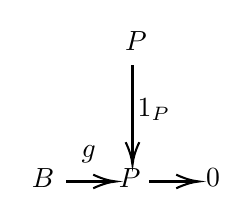
\begin{tikzpicture}[x=0.75pt,y=0.75pt,yscale=-1,xscale=1]
%uncomment if require: \path (0,476); %set diagram left start at 0, and has height of 476

%Straight Lines [id:da9756784236125315] 
\draw    (288,160) -- (288,206) ;
\draw [shift={(288,208)}, rotate = 270] [color={rgb, 255:red, 0; green, 0; blue, 0 }  ][line width=0.75]    (10.93,-3.29) .. controls (6.95,-1.4) and (3.31,-0.3) .. (0,0) .. controls (3.31,0.3) and (6.95,1.4) .. (10.93,3.29)   ;
%Straight Lines [id:da3791632771502693] 
\draw    (256,216) -- (278,216) ;
\draw [shift={(280,216)}, rotate = 180] [color={rgb, 255:red, 0; green, 0; blue, 0 }  ][line width=0.75]    (10.93,-3.29) .. controls (6.95,-1.4) and (3.31,-0.3) .. (0,0) .. controls (3.31,0.3) and (6.95,1.4) .. (10.93,3.29)   ;
%Straight Lines [id:da48034704105691794] 
\draw    (296,216) -- (318,216) ;
\draw [shift={(320,216)}, rotate = 180] [color={rgb, 255:red, 0; green, 0; blue, 0 }  ][line width=0.75]    (10.93,-3.29) .. controls (6.95,-1.4) and (3.31,-0.3) .. (0,0) .. controls (3.31,0.3) and (6.95,1.4) .. (10.93,3.29)   ;

% Text Node
\draw (283,142.4) node [anchor=north west][inner sep=0.75pt]    {$P$};
% Text Node
\draw (238,208.4) node [anchor=north west][inner sep=0.75pt]    {$B$};
% Text Node
\draw (280,208.4) node [anchor=north west][inner sep=0.75pt]    {$P$};
% Text Node
\draw (322,208.4) node [anchor=north west][inner sep=0.75pt]    {$0$};
% Text Node
\draw (289,174.4) node [anchor=north west][inner sep=0.75pt]    {$1_{P}$};
% Text Node
\draw (262,197.4) node [anchor=north west][inner sep=0.75pt]    {$g$};


\end{tikzpicture}
\end{center}
Since $P$ is projective, there exists an $R$-module homomorphism $h:P\to B$ such that $hg=1_P$. Therefore the short exact sequence 
$$0\longrightarrow A\overset{f}{\longrightarrow}B\overset{g}{\longrightarrow}P\longrightarrow 0$$
split, and $B\cong A\oplus P$.\par
(b)$\Rightarrow$(c): Since $F$ is a free module, there exists an epimorphism $g:F\to P$. Let $K=\mathrm{Ker}g$, then we have the short exact sequence 
$$
0\longrightarrow K\longrightarrow F\overset{g}{\longrightarrow}P\longrightarrow 0
$$
is split exact. Therefore $F\cong K\oplus P$.\par
(c)$\Rightarrow$(a): By condition we know that the short exact sequence 
$$
0\longrightarrow K\longrightarrow F\longrightarrow P\longrightarrow 0
$$
split, therefore there exists some $h:P\to F$ such that $hg=1$, here $g:F\to P$ be the canonical injection. Therefore we proved that $P$ is projective.
\end{proof}
We give some examples that are projective modules but not free modules. Consider $\mathbb{Z}_2$ and $\mathbb{Z}_3$. Since $\mathbb{Z}_2$ and $\mathbb{Z}_3$ are $\mathbb{Z}_6$ modules and $\mathbb{Z}_6\cong\mathbb{Z}_2\oplus\mathbb{Z}_3$, we have the short exact sequence 
$$
0\longrightarrow \mathbb{Z} _2\longrightarrow \mathbb{Z} _2\oplus \mathbb{Z} _3\longrightarrow \mathbb{Z} _3\longrightarrow 0
$$
split, and hence by Theorem 5.29 we know that $\mathbb{Z}_2$ and $\mathbb{Z}_3$ are projective but not free $\mathbb{Z}_6$-modules.
\begin{proposition}
Let $R$ be a ring. A direct sum of $R$-modules $\bigoplus_{i\in I}P_i$ is projective if and only if each $P_i$ is projective.
\end{proposition}
\begin{proof}
Suppose $\bigoplus_{i\in I}P_i$ is projective. Then for each $P_j$, we have the following diagram: 
\begin{center}


\tikzset{every picture/.style={line width=0.75pt}} %set default line width to 0.75pt        

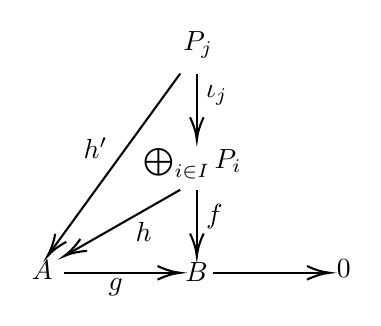
\begin{tikzpicture}[x=0.75pt,y=0.75pt,yscale=-1,xscale=1]
%uncomment if require: \path (0,476); %set diagram left start at 0, and has height of 476

%Straight Lines [id:da4410470739213719] 
\draw    (304,96) -- (304,126) ;
\draw [shift={(304,128)}, rotate = 270] [color={rgb, 255:red, 0; green, 0; blue, 0 }  ][line width=0.75]    (10.93,-3.29) .. controls (6.95,-1.4) and (3.31,-0.3) .. (0,0) .. controls (3.31,0.3) and (6.95,1.4) .. (10.93,3.29)   ;
%Straight Lines [id:da11715093568326385] 
\draw    (304,152) -- (304,182) ;
\draw [shift={(304,184)}, rotate = 270] [color={rgb, 255:red, 0; green, 0; blue, 0 }  ][line width=0.75]    (10.93,-3.29) .. controls (6.95,-1.4) and (3.31,-0.3) .. (0,0) .. controls (3.31,0.3) and (6.95,1.4) .. (10.93,3.29)   ;
%Straight Lines [id:da11098979119714536] 
\draw    (312,192) -- (366,192) ;
\draw [shift={(368,192)}, rotate = 180] [color={rgb, 255:red, 0; green, 0; blue, 0 }  ][line width=0.75]    (10.93,-3.29) .. controls (6.95,-1.4) and (3.31,-0.3) .. (0,0) .. controls (3.31,0.3) and (6.95,1.4) .. (10.93,3.29)   ;
%Straight Lines [id:da38705239794661384] 
\draw    (240,192) -- (294,192) ;
\draw [shift={(296,192)}, rotate = 180] [color={rgb, 255:red, 0; green, 0; blue, 0 }  ][line width=0.75]    (10.93,-3.29) .. controls (6.95,-1.4) and (3.31,-0.3) .. (0,0) .. controls (3.31,0.3) and (6.95,1.4) .. (10.93,3.29)   ;
%Straight Lines [id:da7846735142684917] 
\draw    (296,152) -- (241.74,183.01) ;
\draw [shift={(240,184)}, rotate = 330.26] [color={rgb, 255:red, 0; green, 0; blue, 0 }  ][line width=0.75]    (10.93,-3.29) .. controls (6.95,-1.4) and (3.31,-0.3) .. (0,0) .. controls (3.31,0.3) and (6.95,1.4) .. (10.93,3.29)   ;
%Straight Lines [id:da6462873867895451] 
\draw    (296,96) -- (233.18,182.38) ;
\draw [shift={(232,184)}, rotate = 306.03] [color={rgb, 255:red, 0; green, 0; blue, 0 }  ][line width=0.75]    (10.93,-3.29) .. controls (6.95,-1.4) and (3.31,-0.3) .. (0,0) .. controls (3.31,0.3) and (6.95,1.4) .. (10.93,3.29)   ;

% Text Node
\draw (296,74.4) node [anchor=north west][inner sep=0.75pt]    {$P_{j}$};
% Text Node
\draw (277,130.4) node [anchor=north west][inner sep=0.75pt]    {$\bigoplus _{i\in I} P_{i}$};
% Text Node
\draw (297,185.4) node [anchor=north west][inner sep=0.75pt]    {$B$};
% Text Node
\draw (223,184.4) node [anchor=north west][inner sep=0.75pt]    {$A$};
% Text Node
\draw (370,184.4) node [anchor=north west][inner sep=0.75pt]    {$0$};
% Text Node
\draw (307,157.4) node [anchor=north west][inner sep=0.75pt]    {$f$};
% Text Node
\draw (260,193.4) node [anchor=north west][inner sep=0.75pt]    {$g$};
% Text Node
\draw (273,166.4) node [anchor=north west][inner sep=0.75pt]    {$h$};
% Text Node
\draw (248,125.4) node [anchor=north west][inner sep=0.75pt]    {$h^{\prime }$};
% Text Node
\draw (307,100.4) node [anchor=north west][inner sep=0.75pt]    {$\iota _{j}$};


\end{tikzpicture}
\end{center}
Since $\bigoplus_{i\in I}P_i$ is projective, then there exists some $h$ such that $gh=f$. Now define $h^\prime=h\iota_j$, we have $gh^\prime =gh\iota_j=f\iota_j$, whence $h^\prime$ satisfies the condition and hence $P_j$ is projective. Conversely, we have the following diagram:
\begin{center}


\tikzset{every picture/.style={line width=0.75pt}} %set default line width to 0.75pt        

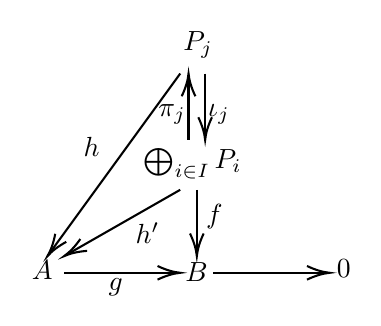
\begin{tikzpicture}[x=0.75pt,y=0.75pt,yscale=-1,xscale=1]
%uncomment if require: \path (0,476); %set diagram left start at 0, and has height of 476

%Straight Lines [id:da4410470739213719] 
\draw    (308,96) -- (308,126) ;
\draw [shift={(308,128)}, rotate = 270] [color={rgb, 255:red, 0; green, 0; blue, 0 }  ][line width=0.75]    (10.93,-3.29) .. controls (6.95,-1.4) and (3.31,-0.3) .. (0,0) .. controls (3.31,0.3) and (6.95,1.4) .. (10.93,3.29)   ;
%Straight Lines [id:da11715093568326385] 
\draw    (304,152) -- (304,182) ;
\draw [shift={(304,184)}, rotate = 270] [color={rgb, 255:red, 0; green, 0; blue, 0 }  ][line width=0.75]    (10.93,-3.29) .. controls (6.95,-1.4) and (3.31,-0.3) .. (0,0) .. controls (3.31,0.3) and (6.95,1.4) .. (10.93,3.29)   ;
%Straight Lines [id:da11098979119714536] 
\draw    (312,192) -- (366,192) ;
\draw [shift={(368,192)}, rotate = 180] [color={rgb, 255:red, 0; green, 0; blue, 0 }  ][line width=0.75]    (10.93,-3.29) .. controls (6.95,-1.4) and (3.31,-0.3) .. (0,0) .. controls (3.31,0.3) and (6.95,1.4) .. (10.93,3.29)   ;
%Straight Lines [id:da38705239794661384] 
\draw    (240,192) -- (294,192) ;
\draw [shift={(296,192)}, rotate = 180] [color={rgb, 255:red, 0; green, 0; blue, 0 }  ][line width=0.75]    (10.93,-3.29) .. controls (6.95,-1.4) and (3.31,-0.3) .. (0,0) .. controls (3.31,0.3) and (6.95,1.4) .. (10.93,3.29)   ;
%Straight Lines [id:da7846735142684917] 
\draw    (296,152) -- (241.74,183.01) ;
\draw [shift={(240,184)}, rotate = 330.26] [color={rgb, 255:red, 0; green, 0; blue, 0 }  ][line width=0.75]    (10.93,-3.29) .. controls (6.95,-1.4) and (3.31,-0.3) .. (0,0) .. controls (3.31,0.3) and (6.95,1.4) .. (10.93,3.29)   ;
%Straight Lines [id:da6462873867895451] 
\draw    (296,96) -- (233.18,182.38) ;
\draw [shift={(232,184)}, rotate = 306.03] [color={rgb, 255:red, 0; green, 0; blue, 0 }  ][line width=0.75]    (10.93,-3.29) .. controls (6.95,-1.4) and (3.31,-0.3) .. (0,0) .. controls (3.31,0.3) and (6.95,1.4) .. (10.93,3.29)   ;
%Straight Lines [id:da7889817906156957] 
\draw    (300,128) -- (300,98) ;
\draw [shift={(300,96)}, rotate = 90] [color={rgb, 255:red, 0; green, 0; blue, 0 }  ][line width=0.75]    (10.93,-3.29) .. controls (6.95,-1.4) and (3.31,-0.3) .. (0,0) .. controls (3.31,0.3) and (6.95,1.4) .. (10.93,3.29)   ;

% Text Node
\draw (296,74.4) node [anchor=north west][inner sep=0.75pt]    {$P_{j}$};
% Text Node
\draw (277,130.4) node [anchor=north west][inner sep=0.75pt]    {$\bigoplus _{i\in I} P_{i}$};
% Text Node
\draw (297,185.4) node [anchor=north west][inner sep=0.75pt]    {$B$};
% Text Node
\draw (223,184.4) node [anchor=north west][inner sep=0.75pt]    {$A$};
% Text Node
\draw (370,184.4) node [anchor=north west][inner sep=0.75pt]    {$0$};
% Text Node
\draw (307,157.4) node [anchor=north west][inner sep=0.75pt]    {$f$};
% Text Node
\draw (260,193.4) node [anchor=north west][inner sep=0.75pt]    {$g$};
% Text Node
\draw (273,166.4) node [anchor=north west][inner sep=0.75pt]    {$h^{\prime }$};
% Text Node
\draw (248,125.4) node [anchor=north west][inner sep=0.75pt]    {$h$};
% Text Node
\draw (308,109.4) node [anchor=north west][inner sep=0.75pt]    {$\iota _{j}$};
% Text Node
\draw (284,109.4) node [anchor=north west][inner sep=0.75pt]    {$\pi _{j}$};


\end{tikzpicture}
\end{center}
Define $h^\prime=\sum_{j\in I}h\pi_j$, then we have 
$$
gh=g\left( \sum_{j\in I}{h\pi _j} \right) =\sum_{j\in I}{gh\pi _j}=\sum_{j\in I}{f\iota _j\pi _j}=f,
$$
which finished the proof.
\end{proof}
Recall that the dual of a concept in category is defined by reversing all arrows. Pushing this idea a bit further one might say that the dual of a monomorphism is epimorphism, since $A\to B$ is monomorphism if and only if $0\longrightarrow A\longrightarrow B$ is exact, and if $A\to B$ is an epimorphism if and only if $B\longrightarrow A\longrightarrow 0$ is exact, which arrows reversed. This leads us to the definition of the dual notion of projective modules in the following way.
\begin{definition}
A module $J$ over a ring $R$ is said to be \textbf{injective} if given any diagram of $R$-module homomorphisms 
\begin{center}


\tikzset{every picture/.style={line width=0.75pt}} %set default line width to 0.75pt        

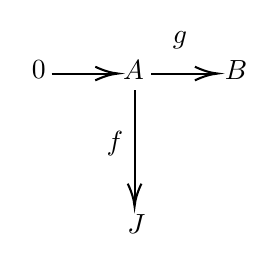
\begin{tikzpicture}[x=0.75pt,y=0.75pt,yscale=-1,xscale=1]
%uncomment if require: \path (0,476); %set diagram left start at 0, and has height of 476

%Straight Lines [id:da2979778987226902] 
\draw    (232,120) -- (262,120) ;
\draw [shift={(264,120)}, rotate = 180] [color={rgb, 255:red, 0; green, 0; blue, 0 }  ][line width=0.75]    (10.93,-3.29) .. controls (6.95,-1.4) and (3.31,-0.3) .. (0,0) .. controls (3.31,0.3) and (6.95,1.4) .. (10.93,3.29)   ;
%Straight Lines [id:da1283630480544964] 
\draw    (280,120) -- (310,120) ;
\draw [shift={(312,120)}, rotate = 180] [color={rgb, 255:red, 0; green, 0; blue, 0 }  ][line width=0.75]    (10.93,-3.29) .. controls (6.95,-1.4) and (3.31,-0.3) .. (0,0) .. controls (3.31,0.3) and (6.95,1.4) .. (10.93,3.29)   ;
%Straight Lines [id:da5874779160595505] 
\draw    (272,128) -- (272,182) ;
\draw [shift={(272,184)}, rotate = 270] [color={rgb, 255:red, 0; green, 0; blue, 0 }  ][line width=0.75]    (10.93,-3.29) .. controls (6.95,-1.4) and (3.31,-0.3) .. (0,0) .. controls (3.31,0.3) and (6.95,1.4) .. (10.93,3.29)   ;

% Text Node
\draw (221,112.4) node [anchor=north west][inner sep=0.75pt]    {$0$};
% Text Node
\draw (265,112.4) node [anchor=north west][inner sep=0.75pt]    {$A$};
% Text Node
\draw (314,112.4) node [anchor=north west][inner sep=0.75pt]    {$B$};
% Text Node
\draw (267,186.4) node [anchor=north west][inner sep=0.75pt]    {$J$};
% Text Node
\draw (289,98.4) node [anchor=north west][inner sep=0.75pt]    {$g$};
% Text Node
\draw (257,146.4) node [anchor=north west][inner sep=0.75pt]    {$f$};


\end{tikzpicture}
\end{center}
with top row exact, i.e., $g$ is an epimorphism, there exists an $R$-module homomorphism $h:B\to J$ such that the diagram 
\begin{center}


\tikzset{every picture/.style={line width=0.75pt}} %set default line width to 0.75pt        

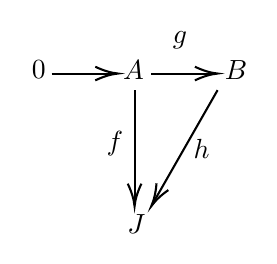
\begin{tikzpicture}[x=0.75pt,y=0.75pt,yscale=-1,xscale=1]
%uncomment if require: \path (0,476); %set diagram left start at 0, and has height of 476

%Straight Lines [id:da2979778987226902] 
\draw    (232,120) -- (262,120) ;
\draw [shift={(264,120)}, rotate = 180] [color={rgb, 255:red, 0; green, 0; blue, 0 }  ][line width=0.75]    (10.93,-3.29) .. controls (6.95,-1.4) and (3.31,-0.3) .. (0,0) .. controls (3.31,0.3) and (6.95,1.4) .. (10.93,3.29)   ;
%Straight Lines [id:da1283630480544964] 
\draw    (280,120) -- (310,120) ;
\draw [shift={(312,120)}, rotate = 180] [color={rgb, 255:red, 0; green, 0; blue, 0 }  ][line width=0.75]    (10.93,-3.29) .. controls (6.95,-1.4) and (3.31,-0.3) .. (0,0) .. controls (3.31,0.3) and (6.95,1.4) .. (10.93,3.29)   ;
%Straight Lines [id:da5874779160595505] 
\draw    (272,128) -- (272,182) ;
\draw [shift={(272,184)}, rotate = 270] [color={rgb, 255:red, 0; green, 0; blue, 0 }  ][line width=0.75]    (10.93,-3.29) .. controls (6.95,-1.4) and (3.31,-0.3) .. (0,0) .. controls (3.31,0.3) and (6.95,1.4) .. (10.93,3.29)   ;
%Straight Lines [id:da03644286916885808] 
\draw    (312,128) -- (280.99,182.26) ;
\draw [shift={(280,184)}, rotate = 299.74] [color={rgb, 255:red, 0; green, 0; blue, 0 }  ][line width=0.75]    (10.93,-3.29) .. controls (6.95,-1.4) and (3.31,-0.3) .. (0,0) .. controls (3.31,0.3) and (6.95,1.4) .. (10.93,3.29)   ;

% Text Node
\draw (221,112.4) node [anchor=north west][inner sep=0.75pt]    {$0$};
% Text Node
\draw (265,112.4) node [anchor=north west][inner sep=0.75pt]    {$A$};
% Text Node
\draw (314,112.4) node [anchor=north west][inner sep=0.75pt]    {$B$};
% Text Node
\draw (267,186.4) node [anchor=north west][inner sep=0.75pt]    {$J$};
% Text Node
\draw (289,98.4) node [anchor=north west][inner sep=0.75pt]    {$g$};
% Text Node
\draw (257,146.4) node [anchor=north west][inner sep=0.75pt]    {$f$};
% Text Node
\draw (299,150.4) node [anchor=north west][inner sep=0.75pt]    {$h$};


\end{tikzpicture}
\end{center}
is commutative, i.e. $hg=f$.
\end{definition}
It is not surprising that many of the preceding propositions about projective modules are readily proved. For example, since the dual of direct sums (coproducts) are products, the dual of Proposition 5.30 is the following:
\begin{proposition}
A direct product of $R$-modules $\prod_{i\in I}J_i$ is injective if and only if each $J_i$ is injective.
\end{proposition}
\begin{proof}
By duality and proposition 5.30, we finished the proof.
\end{proof}
Since the concept of free module can not be dualized, there are no analogues of Theorem 5.27 or Theorem 5.29(iii) for injective modules. However, Corollary 5.28 can be dualized. It states, in effect, that for every module $A$ there is a projective module $P$ and an exact sequence $P\longrightarrow A\longrightarrow 0$. The dual of this statement is that for every module $A$ there is an injective module $J$ and an exact sequence $0\longrightarrow A\longrightarrow J$; in other words, every module may be embedded in an injective module. The remainder of this section is devoted to proving this fact for unitary modules over a ring with identity.
\begin{lemma}\em
Let $R$ be a ring with identity. A unitary $R$-module $J$ is injective if and only if for every left ideal $L$ of $R$, any $R$-module homomorphism $L\to J$ may be extended to an $R$-module homomorphism $R\to J$.
\end{lemma}
\begin{proof}
Suppose $J$ is injective, then we have the following commutative diagram: 
\begin{center}


\tikzset{every picture/.style={line width=0.75pt}} %set default line width to 0.75pt        

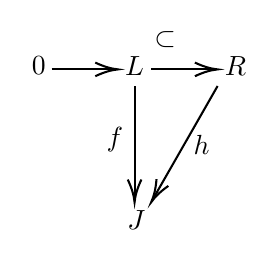
\begin{tikzpicture}[x=0.75pt,y=0.75pt,yscale=-1,xscale=1]
%uncomment if require: \path (0,476); %set diagram left start at 0, and has height of 476

%Straight Lines [id:da2979778987226902] 
\draw    (232,120) -- (262,120) ;
\draw [shift={(264,120)}, rotate = 180] [color={rgb, 255:red, 0; green, 0; blue, 0 }  ][line width=0.75]    (10.93,-3.29) .. controls (6.95,-1.4) and (3.31,-0.3) .. (0,0) .. controls (3.31,0.3) and (6.95,1.4) .. (10.93,3.29)   ;
%Straight Lines [id:da1283630480544964] 
\draw    (280,120) -- (310,120) ;
\draw [shift={(312,120)}, rotate = 180] [color={rgb, 255:red, 0; green, 0; blue, 0 }  ][line width=0.75]    (10.93,-3.29) .. controls (6.95,-1.4) and (3.31,-0.3) .. (0,0) .. controls (3.31,0.3) and (6.95,1.4) .. (10.93,3.29)   ;
%Straight Lines [id:da5874779160595505] 
\draw    (272,128) -- (272,182) ;
\draw [shift={(272,184)}, rotate = 270] [color={rgb, 255:red, 0; green, 0; blue, 0 }  ][line width=0.75]    (10.93,-3.29) .. controls (6.95,-1.4) and (3.31,-0.3) .. (0,0) .. controls (3.31,0.3) and (6.95,1.4) .. (10.93,3.29)   ;
%Straight Lines [id:da03644286916885808] 
\draw    (312,128) -- (280.99,182.26) ;
\draw [shift={(280,184)}, rotate = 299.74] [color={rgb, 255:red, 0; green, 0; blue, 0 }  ][line width=0.75]    (10.93,-3.29) .. controls (6.95,-1.4) and (3.31,-0.3) .. (0,0) .. controls (3.31,0.3) and (6.95,1.4) .. (10.93,3.29)   ;

% Text Node
\draw (221,112.4) node [anchor=north west][inner sep=0.75pt]    {$0$};
% Text Node
\draw (266,112.4) node [anchor=north west][inner sep=0.75pt]    {$L$};
% Text Node
\draw (314,112.4) node [anchor=north west][inner sep=0.75pt]    {$R$};
% Text Node
\draw (267,186.4) node [anchor=north west][inner sep=0.75pt]    {$J$};
% Text Node
\draw (280,100.4) node [anchor=north west][inner sep=0.75pt]    {$\subset $};
% Text Node
\draw (257,146.4) node [anchor=north west][inner sep=0.75pt]    {$f$};
% Text Node
\draw (299,150.4) node [anchor=north west][inner sep=0.75pt]    {$h$};


\end{tikzpicture}
\end{center}
whence there exists some $h:R\to J$ be the extension of $f$. Conversely, suppose $J$ has the properties above, we show that $J$ is injective. Suppose we are given the following diagram 
\begin{center}


\tikzset{every picture/.style={line width=0.75pt}} %set default line width to 0.75pt        

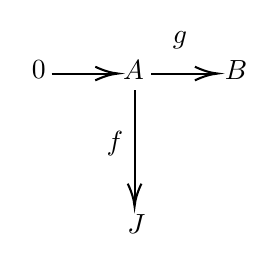
\begin{tikzpicture}[x=0.75pt,y=0.75pt,yscale=-1,xscale=1]
%uncomment if require: \path (0,476); %set diagram left start at 0, and has height of 476

%Straight Lines [id:da2979778987226902] 
\draw    (232,120) -- (262,120) ;
\draw [shift={(264,120)}, rotate = 180] [color={rgb, 255:red, 0; green, 0; blue, 0 }  ][line width=0.75]    (10.93,-3.29) .. controls (6.95,-1.4) and (3.31,-0.3) .. (0,0) .. controls (3.31,0.3) and (6.95,1.4) .. (10.93,3.29)   ;
%Straight Lines [id:da1283630480544964] 
\draw    (280,120) -- (310,120) ;
\draw [shift={(312,120)}, rotate = 180] [color={rgb, 255:red, 0; green, 0; blue, 0 }  ][line width=0.75]    (10.93,-3.29) .. controls (6.95,-1.4) and (3.31,-0.3) .. (0,0) .. controls (3.31,0.3) and (6.95,1.4) .. (10.93,3.29)   ;
%Straight Lines [id:da5874779160595505] 
\draw    (272,128) -- (272,182) ;
\draw [shift={(272,184)}, rotate = 270] [color={rgb, 255:red, 0; green, 0; blue, 0 }  ][line width=0.75]    (10.93,-3.29) .. controls (6.95,-1.4) and (3.31,-0.3) .. (0,0) .. controls (3.31,0.3) and (6.95,1.4) .. (10.93,3.29)   ;

% Text Node
\draw (221,112.4) node [anchor=north west][inner sep=0.75pt]    {$0$};
% Text Node
\draw (265,112.4) node [anchor=north west][inner sep=0.75pt]    {$A$};
% Text Node
\draw (314,112.4) node [anchor=north west][inner sep=0.75pt]    {$B$};
% Text Node
\draw (267,186.4) node [anchor=north west][inner sep=0.75pt]    {$J$};
% Text Node
\draw (289,98.4) node [anchor=north west][inner sep=0.75pt]    {$g$};
% Text Node
\draw (257,146.4) node [anchor=north west][inner sep=0.75pt]    {$f$};


\end{tikzpicture}
\end{center}
with the top row exact. Then we define a collection of $R$-module homomorphisms $\mathcal{S}$, whose elements are homomorphisms $h:C\to J$, where $\mathrm{Im}g\subset C\subset B$. Clearly $\mathcal{S}$ is nonempty, since $fg^{-1}\in\mathcal{S}$. We define the order on $\mathcal{S}$ as follows: We say $h_1\prec h_2$, if $\mathrm{Dom}h_1\subset\mathrm{Dom}h_2$ and $h_2\mid_{\mathrm{Dom}h_1}=h_1$. Then by Zorn's Lemma there exists some maximal element $h:H\to J$. Now it suffices to show that $H=B$.\par
Suppose not, let $b\in B-H$. Then $L=\{r\in R:rb\in H\}$ is a left ideal of $R$. The map $L\to J$ given by $r\mapsto h(rb)$ is a well-defined homomorphism. Therefore by our hypothesis there exists an $R$-module homomorphism $k:R\to J$ such that $k(r)=h(rb)$ for all $r\in R$, as the following diagram shows.
\begin{center}


\tikzset{every picture/.style={line width=0.75pt}} %set default line width to 0.75pt        

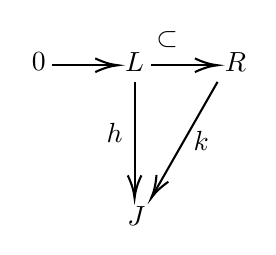
\begin{tikzpicture}[x=0.75pt,y=0.75pt,yscale=-1,xscale=1]
%uncomment if require: \path (0,476); %set diagram left start at 0, and has height of 476

%Straight Lines [id:da2979778987226902] 
\draw    (232,120) -- (262,120) ;
\draw [shift={(264,120)}, rotate = 180] [color={rgb, 255:red, 0; green, 0; blue, 0 }  ][line width=0.75]    (10.93,-3.29) .. controls (6.95,-1.4) and (3.31,-0.3) .. (0,0) .. controls (3.31,0.3) and (6.95,1.4) .. (10.93,3.29)   ;
%Straight Lines [id:da1283630480544964] 
\draw    (280,120) -- (310,120) ;
\draw [shift={(312,120)}, rotate = 180] [color={rgb, 255:red, 0; green, 0; blue, 0 }  ][line width=0.75]    (10.93,-3.29) .. controls (6.95,-1.4) and (3.31,-0.3) .. (0,0) .. controls (3.31,0.3) and (6.95,1.4) .. (10.93,3.29)   ;
%Straight Lines [id:da5874779160595505] 
\draw    (272,128) -- (272,182) ;
\draw [shift={(272,184)}, rotate = 270] [color={rgb, 255:red, 0; green, 0; blue, 0 }  ][line width=0.75]    (10.93,-3.29) .. controls (6.95,-1.4) and (3.31,-0.3) .. (0,0) .. controls (3.31,0.3) and (6.95,1.4) .. (10.93,3.29)   ;
%Straight Lines [id:da4095127738212234] 
\draw    (312,128) -- (280.99,182.26) ;
\draw [shift={(280,184)}, rotate = 299.74] [color={rgb, 255:red, 0; green, 0; blue, 0 }  ][line width=0.75]    (10.93,-3.29) .. controls (6.95,-1.4) and (3.31,-0.3) .. (0,0) .. controls (3.31,0.3) and (6.95,1.4) .. (10.93,3.29)   ;

% Text Node
\draw (221,112.4) node [anchor=north west][inner sep=0.75pt]    {$0$};
% Text Node
\draw (266,112.4) node [anchor=north west][inner sep=0.75pt]    {$L$};
% Text Node
\draw (314,112.4) node [anchor=north west][inner sep=0.75pt]    {$R$};
% Text Node
\draw (267,186.4) node [anchor=north west][inner sep=0.75pt]    {$J$};
% Text Node
\draw (281,102.4) node [anchor=north west][inner sep=0.75pt]    {$\subset $};
% Text Node
\draw (257,146.4) node [anchor=north west][inner sep=0.75pt]    {$h$};
% Text Node
\draw (299,150.4) node [anchor=north west][inner sep=0.75pt]    {$k$};


\end{tikzpicture}
\end{center}
Let $c=k(1_R)$ and define a map $\overline{h}:H+Rb\to J$ given by $a+rb\mapsto h(a)+rc$. Then it is easy to verify that $\overline{h}$ is well-defined and an $R$-module homomorphism. However, $h\prec\overline{h}$, which contradict to the fact that $h$ is a maximal element. Therefore $H=B$, and the proof is finished.
\end{proof}
An abelian group $D$ is said to be \textbf{divisible}, if given any $y\in D$ and $0\ne n\in\mathbb{Z}$, there exists $x\in D$ such that $nx=y$. For example, the additive group $\mathbb{Q}$ is divisible. However $\mathbb{Z}$ is not. The next lemma gives a characterization of divisible groups.
\begin{lemma}\em
An abelian group $D$ is divisible if and only if $D$ is an injective (unitary) $\mathbb{Z}$-module.
\end{lemma}
\begin{proof}
Suppose $D$ is divisible. Then let $y\in D$ and $0\ne n\in\mathbb{Z}$, we consider the homomorphism $f:\left<n\right>\to D$ determined by $n\mapsto y$. Since $D$ is injective, there is a homomorphism $h:\mathbb{Z}\to D$ such that the diagram 
\begin{center}


\tikzset{every picture/.style={line width=0.75pt}} %set default line width to 0.75pt        

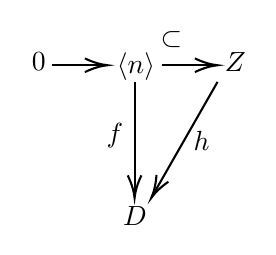
\begin{tikzpicture}[x=0.75pt,y=0.75pt,yscale=-1,xscale=1]
%uncomment if require: \path (0,476); %set diagram left start at 0, and has height of 476

%Straight Lines [id:da2979778987226902] 
\draw    (232,120) -- (257,120) ;
\draw [shift={(259,120)}, rotate = 180] [color={rgb, 255:red, 0; green, 0; blue, 0 }  ][line width=0.75]    (10.93,-3.29) .. controls (6.95,-1.4) and (3.31,-0.3) .. (0,0) .. controls (3.31,0.3) and (6.95,1.4) .. (10.93,3.29)   ;
%Straight Lines [id:da1283630480544964] 
\draw    (285,120) -- (310,120) ;
\draw [shift={(312,120)}, rotate = 180] [color={rgb, 255:red, 0; green, 0; blue, 0 }  ][line width=0.75]    (10.93,-3.29) .. controls (6.95,-1.4) and (3.31,-0.3) .. (0,0) .. controls (3.31,0.3) and (6.95,1.4) .. (10.93,3.29)   ;
%Straight Lines [id:da5874779160595505] 
\draw    (272,128) -- (272,182) ;
\draw [shift={(272,184)}, rotate = 270] [color={rgb, 255:red, 0; green, 0; blue, 0 }  ][line width=0.75]    (10.93,-3.29) .. controls (6.95,-1.4) and (3.31,-0.3) .. (0,0) .. controls (3.31,0.3) and (6.95,1.4) .. (10.93,3.29)   ;
%Straight Lines [id:da4095127738212234] 
\draw    (312,128) -- (280.99,182.26) ;
\draw [shift={(280,184)}, rotate = 299.74] [color={rgb, 255:red, 0; green, 0; blue, 0 }  ][line width=0.75]    (10.93,-3.29) .. controls (6.95,-1.4) and (3.31,-0.3) .. (0,0) .. controls (3.31,0.3) and (6.95,1.4) .. (10.93,3.29)   ;

% Text Node
\draw (221,112.4) node [anchor=north west][inner sep=0.75pt]    {$0$};
% Text Node
\draw (262,112.4) node [anchor=north west][inner sep=0.75pt]    {$\left<n\right>$};
% Text Node
\draw (314,112.4) node [anchor=north west][inner sep=0.75pt]    {$\mathbb{Z}$};
% Text Node
\draw (265,186.4) node [anchor=north west][inner sep=0.75pt]    {$D$};
% Text Node
\draw (283,102.4) node [anchor=north west][inner sep=0.75pt]    {$\subset $};
% Text Node
\draw (257,146.4) node [anchor=north west][inner sep=0.75pt]    {$f$};
% Text Node
\draw (299,150.4) node [anchor=north west][inner sep=0.75pt]    {$h$};


\end{tikzpicture}
\end{center}
is commutative. Let $h(1)=x$, then $nx=nh(1)=h(n)=y$, whence $D$ is divisible. Conversely, suppose $D$ is divisible, then since the ideal of $\mathbb{Z}$ are of the form $\left<n\right>$, then there exists some $x\in D$ such that $nx=f(n)$, where $f:\left<n\right>$ is the homomorphism defined by $n\mapsto a_x$. Define $h:\mathbb{Z}\to D$ by $1\mapsto x$, therefore $h$ is the extension of $f$, whence $D$ is injective by Lemma 5.4.
\end{proof}
\begin{lemma}\em
Every abelian group $A$ may be embedded in a divisible abelian group.
\end{lemma}
\begin{proof}
Since $A$ is an abelian group, we know that $A$ is a $\mathbb{Z}$-module, and hence a homomorphic image of some free $\mathbb{Z}$-module $F$. Therefore $A\cong F/K$. Note that $F\cong\bigoplus\mathbb{Z}$, and each $\mathbb{Z}$ can be embedded into the divisible group $\mathbb{Q}$, therefore 
$$
A\cong F/K\cong \left( \bigoplus{\mathbb{Z}} \right) /K\subset \left( \bigoplus{\mathbb{Q}} \right) /K
$$
and hence $A$ can be embedded into $\left(\bigoplus\mathbb{Q}\right)/K$. Observe that $\left(\bigoplus\mathbb{Q}\right)/K$ is also a divisible group.
\end{proof}
If $R$ is a ring with identity and $J$ is an abelian group, then $\mathrm{Hom}_\mathbb{Z}(R,J)$, the set of all $\mathbb{Z}$-module homomorphisms $R\to J$, is an abelian group. It is easy to verify that $\mathrm{Hom}_\mathbb{Z}(R,J)$ is a unitary $R$-module with the action of $R$ defined by $(rf)(x)=f(xr)$, where $r,x\in R$ and $f\in\mathrm{Hom}_\mathbb{Z}(R,J)$.
\begin{lemma}\em
If $J$ is a divisible abelian group and $R$ is a ring with identity, then $\mathrm{Hom}_\mathbb{Z}(R,J)$ is an injective $R$-module.
\end{lemma}
\begin{proof}
Let $L$ be a left ideal of $R$ and $f:L\to\mathrm{Hom}_\mathbb{Z}(R,J)$ be an $R$-module homomorphism. It suffices to show that there exists an extension $h:R\to\mathrm{Hom}_\mathbb{Z}(R,J)$. Now since $J$ is a divisible abelian group, it is an injective $\mathbb{Z}$-module. Let $g:a\mapsto[f(a)]1_R$, therefore we have the following diagram: 
\begin{center}


\tikzset{every picture/.style={line width=0.75pt}} %set default line width to 0.75pt        

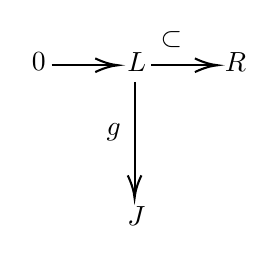
\begin{tikzpicture}[x=0.75pt,y=0.75pt,yscale=-1,xscale=1]
%uncomment if require: \path (0,476); %set diagram left start at 0, and has height of 476

%Straight Lines [id:da2979778987226902] 
\draw    (232,120) -- (262,120) ;
\draw [shift={(264,120)}, rotate = 180] [color={rgb, 255:red, 0; green, 0; blue, 0 }  ][line width=0.75]    (10.93,-3.29) .. controls (6.95,-1.4) and (3.31,-0.3) .. (0,0) .. controls (3.31,0.3) and (6.95,1.4) .. (10.93,3.29)   ;
%Straight Lines [id:da1283630480544964] 
\draw    (280,120) -- (310,120) ;
\draw [shift={(312,120)}, rotate = 180] [color={rgb, 255:red, 0; green, 0; blue, 0 }  ][line width=0.75]    (10.93,-3.29) .. controls (6.95,-1.4) and (3.31,-0.3) .. (0,0) .. controls (3.31,0.3) and (6.95,1.4) .. (10.93,3.29)   ;
%Straight Lines [id:da5874779160595505] 
\draw    (272,128) -- (272,182) ;
\draw [shift={(272,184)}, rotate = 270] [color={rgb, 255:red, 0; green, 0; blue, 0 }  ][line width=0.75]    (10.93,-3.29) .. controls (6.95,-1.4) and (3.31,-0.3) .. (0,0) .. controls (3.31,0.3) and (6.95,1.4) .. (10.93,3.29)   ;

% Text Node
\draw (221,112.4) node [anchor=north west][inner sep=0.75pt]    {$0$};
% Text Node
\draw (267,112.4) node [anchor=north west][inner sep=0.75pt]    {$L$};
% Text Node
\draw (314,112.4) node [anchor=north west][inner sep=0.75pt]    {$R$};
% Text Node
\draw (267,186.4) node [anchor=north west][inner sep=0.75pt]    {$J$};
% Text Node
\draw (283,102.4) node [anchor=north west][inner sep=0.75pt]    {$\subset $};
% Text Node
\draw (257,146.4) node [anchor=north west][inner sep=0.75pt]    {$g$};


\end{tikzpicture}
\end{center}
Now since $J$ is an injective module over $\mathbb{Z}$, there exists some extension of $g$, denote as $\overline{g}:R\to J$. We now define $h:R\to\mathrm{Hom}_\mathbb{Z}(R,J)$ to be $r\mapsto h(r)$, where $h(r)(x)=\overline{g}(xr)$. It is easy to verify that $h(r)\in\mathrm{Hom}_\mathbb{Z}(R,J)$ and hence $h:R\to\mathrm{Hom}_\mathbb{Z}(R,J)$. Now suppose $r\in L$ and $x\in R$. Then $xr\in L$ and 
$$
h\left( r \right) \left( x \right) =\overline{g}\left( xr \right) =g\left( xr \right) =\left[ f\left( xr \right) \right] 1_R=\left[ xf\left( r \right) \right] 1_R=f\left( r \right) \left( 1_Rx \right) =f\left( r \right) \left( x \right) ,
$$
therefore $h(r)=f(r)$, and the proof is finished.
\end{proof}
We are now able to proof the duals of Corollary 5.28 and Theorem 5.29.
\begin{proposition}
Every unitary module $A$ over a ring $R$ with identity may be embedded in an injective $R$-module.
\end{proposition}
\begin{proof}
First since $A$ is an abelian group, there exists some divisible abelian groups $J$ such that $A$ may be embedded in $J$. Define the $R$-module monomorphism $f:A\to J$. Then we consider $\overline{f}:\mathrm{Hom}_\mathbb{Z}(R,A)\to\mathrm{Hom}_\mathbb{Z}(R,J)$ given by $g\mapsto fg$, where $g\in\mathrm{Hom}_\mathbb{Z}(R,A)$. It is easy to verify that $\overline{f}$ is also an $R$-module monomorphism. Note that every $R$-module homomorphism is also a $\mathbb{Z}$-module homomorphism, which due to the fact that every $R$-module is an abelian group, and hence a $\mathbb{Z}$-module, we obtain the inclusion $\mathrm{Hom}_R(R,A)\subset\mathrm{Hom}_\mathbb{Z}(R,A)$. Observe that $A$ may be embedded into $\mathrm{Hom}_R(R,A)$, which suffices to note that the map $g:A\to\mathrm{Hom}_R(R,A)$ given by $a\mapsto f_a$, where $f_a$ is defined to be $f_a(r)=ra$, is a monomorphism, we have the following composition: 
$$
A\overset{g}{\longrightarrow}\mathrm{Hom}_R\left( R,A \right) \overset{\subset}{\longrightarrow}\mathrm{Hom}_{\mathbb{Z}}\left( R,A \right) \overset{\overline{f}}{\longrightarrow}\mathrm{Hom}_{\mathbb{Z}}\left( R,J \right) ,
$$
we conclude that $A$ may be embedded into $\mathrm{Hom}_\mathbb{Z}(R,J)$, where the latter one is, by Lemma 5.7, an injective $R$-module.
\end{proof}
\begin{proposition}
Let $R$ be a ring with identity. The following conditions on a unitary $R$-module $J$ are equivalent.\par
(a) $J$ is injective;\par
(b) every short exact sequence $0\longrightarrow J\overset{f}{\longrightarrow}B\overset{g}{\longrightarrow}C\longrightarrow 0$ is split exact;\par
(c) $J$ is the direct summand of any module $B$ of which it is a submodule.
\end{proposition}
\begin{proof}
(a)$\Rightarrow$(b): Dualize the proof of Theorem 5.29.\par
(b)$\Rightarrow$(c): Consider the short exact sequence 
$$
0\longrightarrow J\overset{\subset}{\longrightarrow}B\overset{\pi}{\longrightarrow}B/J\longrightarrow 0,
$$
therefore since the short exact sequence is split exact, we have $B\cong J\oplus B/J$, whence $J$ is a direct summand of $B$.\par
(c)$\Rightarrow$(a): It follows from Proposition 5.33 that $J$ is a submodule of some injective module $Q$. Proposition 5.32 and (c) implies that $J$ is injective.
\end{proof}
\begin{center}
\begin{large}
    \textbf{Exercises for 5.3}
\end{large}
\end{center}
Note: $R$ is a ring. If $R$ has an identity, all $R$-modules are assumed to be unitary.
\begin{problem}\em
The following conditions on a ring $R$ [with identity] are equivalent:\par
(a) Every [unitary] $R$-module is projective.\par
(b) Every short exact sequence of [unitary] $R$-modules is split exact.\par
(c) Every [unitary] $R$-module is injective.
\end{problem}
\begin{proof}
We first show that (a) and (b) are equivalent.\par
(a)$\Rightarrow$(b): Note that the following diagram 
\begin{center}


\tikzset{every picture/.style={line width=0.75pt}} %set default line width to 0.75pt        

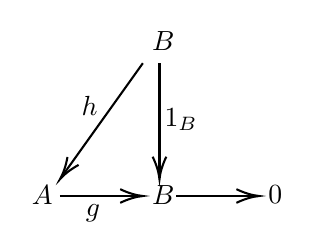
\begin{tikzpicture}[x=0.75pt,y=0.75pt,yscale=-1,xscale=1]
%uncomment if require: \path (0,476); %set diagram left start at 0, and has height of 476

%Straight Lines [id:da22892850871398007] 
\draw    (208,192) -- (246,192) ;
\draw [shift={(248,192)}, rotate = 180] [color={rgb, 255:red, 0; green, 0; blue, 0 }  ][line width=0.75]    (10.93,-3.29) .. controls (6.95,-1.4) and (3.31,-0.3) .. (0,0) .. controls (3.31,0.3) and (6.95,1.4) .. (10.93,3.29)   ;
%Straight Lines [id:da815882418865653] 
\draw    (264,192) -- (302,192) ;
\draw [shift={(304,192)}, rotate = 180] [color={rgb, 255:red, 0; green, 0; blue, 0 }  ][line width=0.75]    (10.93,-3.29) .. controls (6.95,-1.4) and (3.31,-0.3) .. (0,0) .. controls (3.31,0.3) and (6.95,1.4) .. (10.93,3.29)   ;
%Straight Lines [id:da20936486711467128] 
\draw    (256,128) -- (256,182) ;
\draw [shift={(256,184)}, rotate = 270] [color={rgb, 255:red, 0; green, 0; blue, 0 }  ][line width=0.75]    (10.93,-3.29) .. controls (6.95,-1.4) and (3.31,-0.3) .. (0,0) .. controls (3.31,0.3) and (6.95,1.4) .. (10.93,3.29)   ;
%Straight Lines [id:da9215006364241813] 
\draw    (248,128) -- (209.16,182.37) ;
\draw [shift={(208,184)}, rotate = 305.54] [color={rgb, 255:red, 0; green, 0; blue, 0 }  ][line width=0.75]    (10.93,-3.29) .. controls (6.95,-1.4) and (3.31,-0.3) .. (0,0) .. controls (3.31,0.3) and (6.95,1.4) .. (10.93,3.29)   ;

% Text Node
\draw (193,185.4) node [anchor=north west][inner sep=0.75pt]    {$A$};
% Text Node
\draw (251,185.4) node [anchor=north west][inner sep=0.75pt]    {$B$};
% Text Node
\draw (307,185.4) node [anchor=north west][inner sep=0.75pt]    {$0$};
% Text Node
\draw (251,111.4) node [anchor=north west][inner sep=0.75pt]    {$B$};
% Text Node
\draw (257,148.4) node [anchor=north west][inner sep=0.75pt]    {$1_{B}$};
% Text Node
\draw (219,194.4) node [anchor=north west][inner sep=0.75pt]    {$g$};
% Text Node
\draw (217,142.4) node [anchor=north west][inner sep=0.75pt]    {$h$};


\end{tikzpicture}
\end{center}
is commutative, there exists some $h:B\to A$ and hence the short exact sequence is split exact.\par
(b)$\Rightarrow$(a): Since every short exact sequence of $R$-modules is split exact, then the short exact sequence 
$$
0\longrightarrow A\overset{f}{\longrightarrow}B\overset{g}{\longrightarrow}P\longrightarrow 0
$$
is split exact, hence $P$ is a projective module.\par
We now show that (b) and (c) are equivalent, and hence the proof is finished.\par
(b)$\Rightarrow$(c): Since every short exact sequence of $R$-modules is split exact, then the short exact sequence 
$$
0\longrightarrow J\overset{f}{\longrightarrow}A\overset{g}{\longrightarrow}B\longrightarrow 0
$$
is split exact, hence $J$ is an injective module.\par
(c)$\Rightarrow$(b): Note that the following diagram 
\begin{center}


\tikzset{every picture/.style={line width=0.75pt}} %set default line width to 0.75pt        

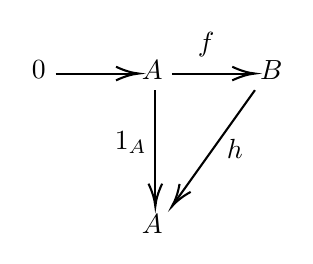
\begin{tikzpicture}[x=0.75pt,y=0.75pt,yscale=-1,xscale=1]
%uncomment if require: \path (0,476); %set diagram left start at 0, and has height of 476

%Straight Lines [id:da5937754556996264] 
\draw    (200,112) -- (238,112) ;
\draw [shift={(240,112)}, rotate = 180] [color={rgb, 255:red, 0; green, 0; blue, 0 }  ][line width=0.75]    (10.93,-3.29) .. controls (6.95,-1.4) and (3.31,-0.3) .. (0,0) .. controls (3.31,0.3) and (6.95,1.4) .. (10.93,3.29)   ;
%Straight Lines [id:da0029257347153581748] 
\draw    (256,112) -- (294,112) ;
\draw [shift={(296,112)}, rotate = 180] [color={rgb, 255:red, 0; green, 0; blue, 0 }  ][line width=0.75]    (10.93,-3.29) .. controls (6.95,-1.4) and (3.31,-0.3) .. (0,0) .. controls (3.31,0.3) and (6.95,1.4) .. (10.93,3.29)   ;
%Straight Lines [id:da8317479595227399] 
\draw    (248,120) -- (248,174) ;
\draw [shift={(248,176)}, rotate = 270] [color={rgb, 255:red, 0; green, 0; blue, 0 }  ][line width=0.75]    (10.93,-3.29) .. controls (6.95,-1.4) and (3.31,-0.3) .. (0,0) .. controls (3.31,0.3) and (6.95,1.4) .. (10.93,3.29)   ;
%Straight Lines [id:da6461060090515085] 
\draw    (296,120) -- (257.16,174.37) ;
\draw [shift={(256,176)}, rotate = 305.54] [color={rgb, 255:red, 0; green, 0; blue, 0 }  ][line width=0.75]    (10.93,-3.29) .. controls (6.95,-1.4) and (3.31,-0.3) .. (0,0) .. controls (3.31,0.3) and (6.95,1.4) .. (10.93,3.29)   ;

% Text Node
\draw (187,104.4) node [anchor=north west][inner sep=0.75pt]    {$0$};
% Text Node
\draw (240,104.4) node [anchor=north west][inner sep=0.75pt]    {$A$};
% Text Node
\draw (297,104.4) node [anchor=north west][inner sep=0.75pt]    {$B$};
% Text Node
\draw (240,178.4) node [anchor=north west][inner sep=0.75pt]    {$A$};
% Text Node
\draw (267,90.4) node [anchor=north west][inner sep=0.75pt]    {$f$};
% Text Node
\draw (281,142.4) node [anchor=north west][inner sep=0.75pt]    {$h$};
% Text Node
\draw (227,138.4) node [anchor=north west][inner sep=0.75pt]    {$1_{A}$};


\end{tikzpicture}
\end{center}
is commutative, there exists some $h:B\to A$ and hence the short exact sequence is split exact.
\end{proof}
\begin{problem}\em
Let $R$ be a ring with identity. An $R$-module $A$ is injective if and only if for every left ideal $L$ of $R$ and $R$-module homomorphism $g:L\to A$, there exists $a\in A$ such that $g(r)=ra$ for every $r\in L$.
\end{problem}
\begin{proof}
Suppose $A$ is an injective $R$-module, then there exists an extension $h:R\to A$ of $g$, hence 
$$
g\left( r \right) =h\left( r \right) =h\left( r\cdot 1_R \right) =h\left( 1_R \right) r,
$$
let $h(1_R)=a$. Conversely, since $L$ is an ideal of $R$, we have $rl\in L$ for all $r\in R$ and $l\in L$. Therefore $g\left( rl \right) =rg\left( l \right) =rla$ defines an extension of $g$, and hence $A$ is injective.
\end{proof}
\begin{problem}\em
Every vector space over a division ring $D$ is both a projective and injective $D$-module.
\end{problem}
\begin{proof}
Since every vector space has a basis, we know that $V$ is a free $D$-module, therefore a projective module. By Exercise 5.26 we know that $V$ is also an injective module.
\end{proof}
\begin{problem}\em
(a) For each prime $p$, $\mathbb{Z}(p^\infty)$ is a divisible group.\par
(b) No nonzero finite abelian group is divisible.\par
(c) No nonzero free abelian group is divisible.\par
(d) $\mathbb{Q}$ is an injective $\mathbb{Z}$-module.
\end{problem}
\begin{proof}
(a) Let $\overline{a/p^l}\in\mathbb{Z}(p^\infty)$ and $n\in\mathbb{Z}$ an integer. We show that there exists some $y\in\mathbb{Z}(p^\infty)$ such that $ny=x$. Suppose $n=p^mr$. Then $r$ is an invertible element in $\mathbb{Z}/p^i\mathbb{Z}$ since $(r,p)=1$, whence there exists some $s\in\mathbb{Z}$ such that $rs\equiv 1(\mathrm{mod}p^i)$. Let $y=\overline{as/p^{m+l}}$, then 
$$
ny=n\cdot \overline{as/p^{m+l}}=p^mr\cdot \overline{as/p^{m+l}}=\overline{ars/p^l}=\overline{a/p^l}=x,
$$
whence $\mathbb{Z}(p^\infty)$ is divisible.\par
(b) Suppose $A$ is a finite abelian group. Then $A\cong\bigoplus\mathbb{Z}/p^i\mathbb{Z}$ for some prime $p$ and $i\in\mathbb{Z}$. We show that $\mathbb{Z}/p^i\mathbb{Z}$ are not injective modules. Consider the short exact sequence 
$$
0\longrightarrow p^i\mathbb{Z} /p^{2i}\mathbb{Z} \longrightarrow \mathbb{Z} /p^{2i}\mathbb{Z} \longrightarrow \mathbb{Z} /p^i\mathbb{Z} \longrightarrow 0
$$
where each homomorphism is the canonical injection. It is not spilt exact since 
$$
\mathbb{Z} /p^{2i}\mathbb{Z} \ncong p^i\mathbb{Z} /p^{2i}\mathbb{Z} \oplus \mathbb{Z} /p^i\mathbb{Z} ,
$$
whence $\mathbb{Z}/p^i\mathbb{Z}$ is not injective $\mathbb{Z}$-module, so is $A$.\par
(c) Suppose $F$ is a free abelian group. Then $F\cong\bigoplus\mathbb{Z}$. We show that $\mathbb{Z}$ is not an injective $\mathbb{Z}$-module. Consider the short exact sequence 
$$
0\longrightarrow \mathbb{Z} \longrightarrow \mathbb{Z} \oplus 2\mathbb{Z} \longrightarrow \mathbb{Z} \longrightarrow 0
$$
with the first arrow canonical injection and the second $2k\mapsto k$. It is not split exact since 
$$
\mathbb{Z} \oplus 2\mathbb{Z} \ncong \mathbb{Z} \oplus \mathbb{Z} .
$$
Therefore $F$ is not an injective $\mathbb{Z}$-module.\par
(d) We proof by using Exercise 5.27. Consider a $\mathbb{Z}$-module homomorphism $g:n\mathbb{Z}\to\mathbb{Q}$, where $n\mathbb{Z}$ is an ideal of $\mathbb{Z}$. Since $\mathbb{Q}$ is divisible, there exists some $y\in\mathbb{Q}$ such that $ky=g(k)$ for all $k\in n\mathbb{Z}$. Therefore $g$ may be extended onto $\mathbb{Z}$ and hence $\mathbb{Q}$ an injective $\mathbb{Z}$-module.
\end{proof}
\begin{problem}\em
$\mathbb{Q}$ is not projective $\mathbb{Z}$-module.
\end{problem}
\begin{proof}
Note that a module is projective over principal ideal domain if and only if it is free (which will be introduced in section 5.6), if $\mathbb{Q}$ is projective, then $\mathbb{Q}$ is a free $\mathbb{Z}$-module. However $\mathbb{Q}$ is not free over $\mathbb{Z}$, a contradiction!
\end{proof}
\begin{problem}\em
If $G$ is an abelian group, then $G\cong D\oplus N$, with $D$ divisible and $N$ \textbf{reduced}, i.e., $N$ has no nontrivial divisible subgroups.
\end{problem}
\begin{proof}
Suppose $\{D_i\}_{i\in I}$ is the collection of all subgroups of $G$ such that $D_i$ is divisible, and let $D=\left<\bigcup_{i\in I}D_i\right>$. Since $G$ is an abelian group, we have $D\lhd G$. Let $N=G/D$, then $G\cong D\oplus N$, we finished the proof.
\end{proof}
\begin{problem}\em
Every torsion-free divisible abelian group $D$ is a direct sum of copies of the rationals $\mathbb{Q}$.
\end{problem}
\begin{proof}
We show that $D$ is a vector space over $\mathbb{Q}$. To see this, observe that $D$ is divisible, hence for all $x\in D$, there exists some $y\in D$ such that $ny=x$. Denote $y=(1/n)x$ and $my=(m/n)x$. Since $D$ is torsion-free, we have $r_1x=r_2x$ if and only if $r_1=r_2$. By easy verification of definition one may show that $D$ is a vector space over $\mathbb{Q}$, whence $D$ has a basis $X$. Suppose $r\in D$ and $r=\sum_{i\in I}k_ix_i$, where $r_i\in X$ and $k_i\in\mathbb{Q}$, therefore there exists a correspondence that $r\mapsto(k_1,k_2,\cdots)\in\bigoplus_{i\in I}\mathbb{Q}$. Since the correspondence is one-to-one, we showed that $D\cong\bigoplus\mathbb{Q}$.
\end{proof}
\begin{problem}\em
(a) If $D$ is an abelian group with torsion subgroup $D_t$, then $D/D_t$ is torsion free.\par
(b) If $D$ is divisible, then so is $D_t$, whence $D\cong D_t\oplus E$, where $E$ is torsion free.
\end{problem}
\begin{proof}
(a) Suppose $a+D_t\in D/D_t$. If $a+D_t$ has finite order, then there exists some $n\in\mathbb{Z}$ such that $na+D_t=0+D_t$, whence $na\in D_t$. Since $D_t$ is torsion group, there exists some $m\in\mathbb{Z}$ such that $mna=0$, whence $a\in D_t$ and hence $a+D_t=0+D_t$.\par
(b) Suppose $D$ is divisible. Let $y\in D_t$. Since $D_t$ is a subgroup of $D$ and $D$ is divisible, there exists some $x\in D$ such that $nx=y$ with $n\in\mathbb{Z}$. However $y\in D_t$, whence $my=0$ for some $m\in\mathbb{Z}$, hence $mnx=0$, whence $x\in D_t$ and this implies $D_t$ divisible. By Exercise 5.31 we finished the proof.
\end{proof}
\begin{problem}\em
Let $p$ be a prime and $D$ a divisible abelian $p$-group. Then $D$ is a direct sum of copies of $\mathbb{Z}(p^\infty)$.
\end{problem}
\begin{proof}
We consider $D[p]$ as a vector space of $\mathbb{Z}/(p)=\mathbb{Z}_p$, see exercise 5.18. Let $X$ be the basis of $D[p]$. Since $D$ is a divisible abelian $p$-group, then for all $x\in X$, there exists some $x_1\in X$ such that $|x_1|=p$. Now since $D$ is divisible, there exists some $x_2=px_1,\cdots,x_{n+1}=px_n,\cdots$. Now suppose $H_x$ is generated by $x_1,x_2,\cdots$, by Exercise 2.36 we have $H_x\cong\mathbb{Z}(p^\infty)$. Therefore $D\cong\bigoplus H_x\cong\bigoplus\mathbb{Z}(p^\infty)$.
\end{proof}
\begin{problem}\em
Every divisible abelian group is a direct sum of copies of the rationals $\mathbb{Q}$ and copies of $\mathbb{Z}(p^\infty)$ for various primes $p$.
\end{problem}
\begin{proof}
Let $G_t$ be a torsion subgroup of $G$, then $G_t$ is divisible. Hence by Exercise 5.33 there exists some $E$ that is torsion-free such that $G\cong G_t\oplus E$. For $E$, it is divisible and torsion-free, therefore by Exercise 5.32 we know that $E\cong\bigoplus\mathbb{Q}$. Now for $G_t$, since it is a torsion group, it is the direct sum of some $p$-groups. By Exercise 5.34 we know that each $p$-group is the direct sum of some $\mathbb{Z}(p^\infty)$, therefore 
$$
G\cong G_t\oplus E\cong \left( \bigoplus_{p\in \mathcal{P}}{G_p} \right) \oplus \left( \bigoplus{\mathbb{Q}} \right) \cong \left( \bigoplus_{p\in \mathcal{P}}{\mathbb{Z} \left( p^{\infty} \right)} \right) \oplus \left( \bigoplus{\mathbb{Q}} \right) ,
$$
which finished the proof.
\end{proof}
\begin{problem}\em
Let $G,H,K$ be divisible abelian groups.\par
(a) If $G\oplus G\cong H\oplus H$, then $G\cong H$.\par
(b) If $G\oplus K\cong H\oplus K$, then $H\cong K$.
\end{problem}
\begin{proof}
(a) By Exercise 5.35, this is trivial.\par
(b) By Exercise 5.35, we may deduce the consequence into that of finite abelian groups, whence the proof is finished.
\end{proof}
\subsection{Hom and Duality}
Recall that if $A$ and $B$ are modules over a ring $R$, then $\mathrm{Hom}_R(A,B)$ is the set of all $R$-module homomorphisms $f:A\to B$. If $R=\mathbb{Z}$ we shall usually write $\mathrm{Hom}(A,B)$ rather than $\mathrm{Hom}_\mathbb{Z}(A,B)$. $\mathrm{Hom}_R(A,B)$ is an abelian group under addition and this addition is distributive with respect to composition of functions.
\begin{theorem}
Let $A,B,C,D$ be modules over a ring $R$ and $\varphi:C\to A$ and $\psi:B\to D$ $R$-module homomorphisms. Then the map $\theta:\mathrm{Hom}_R(A,B)\to\mathrm{Hom}_R(C,D)$ given by $f\mapsto\psi f\varphi$ is a homomorphism of abelian groups.
\end{theorem}
\begin{proof}
The map $\theta$ is first well-defined since composition of $R$-module homomorphisms is a homomorphism. It is then an $R$-module homomorphism since the composition of homomorphisms is distributive with respect to addition.
\end{proof}
The homomorphism $\theta$ is usually denoted $\mathrm{Hom}(\varphi,\psi)$ and called homomorphism induced by $\varphi$ and $\psi$, see the following diagram:
\begin{center}


\tikzset{every picture/.style={line width=0.75pt}} %set default line width to 0.75pt        

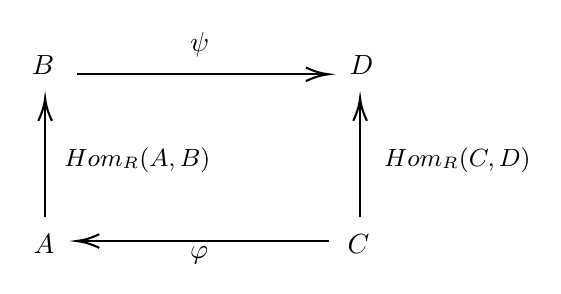
\begin{tikzpicture}[x=0.75pt,y=0.75pt,yscale=-1,xscale=1]
%uncomment if require: \path (0,476); %set diagram left start at 0, and has height of 476

%Straight Lines [id:da2920246208679915] 
\draw    (191.18,237.57) -- (191.18,182.17) ;
\draw [shift={(191.18,180.17)}, rotate = 90] [color={rgb, 255:red, 0; green, 0; blue, 0 }  ][line width=0.75]    (10.93,-3.29) .. controls (6.95,-1.4) and (3.31,-0.3) .. (0,0) .. controls (3.31,0.3) and (6.95,1.4) .. (10.93,3.29)   ;
%Straight Lines [id:da04506002983020263] 
\draw    (342.93,237.57) -- (342.93,182.17) ;
\draw [shift={(342.93,180.17)}, rotate = 90] [color={rgb, 255:red, 0; green, 0; blue, 0 }  ][line width=0.75]    (10.93,-3.29) .. controls (6.95,-1.4) and (3.31,-0.3) .. (0,0) .. controls (3.31,0.3) and (6.95,1.4) .. (10.93,3.29)   ;
%Straight Lines [id:da37803238364229985] 
\draw    (206.35,168.7) -- (325.75,168.7) ;
\draw [shift={(327.75,168.7)}, rotate = 180] [color={rgb, 255:red, 0; green, 0; blue, 0 }  ][line width=0.75]    (10.93,-3.29) .. controls (6.95,-1.4) and (3.31,-0.3) .. (0,0) .. controls (3.31,0.3) and (6.95,1.4) .. (10.93,3.29)   ;
%Straight Lines [id:da5428498747387094] 
\draw    (327.75,249.04) -- (208.35,249.04) ;
\draw [shift={(206.35,249.04)}, rotate = 360] [color={rgb, 255:red, 0; green, 0; blue, 0 }  ][line width=0.75]    (10.93,-3.29) .. controls (6.95,-1.4) and (3.31,-0.3) .. (0,0) .. controls (3.31,0.3) and (6.95,1.4) .. (10.93,3.29)   ;

% Text Node
\draw (183.28,158.23) node [anchor=north west][inner sep=0.75pt]    {$B$};
% Text Node
\draw (336.38,158.23) node [anchor=north west][inner sep=0.75pt]    {$D$};
% Text Node
\draw (184.18,244.31) node [anchor=north west][inner sep=0.75pt]    {$A$};
% Text Node
\draw (335.48,244.31) node [anchor=north west][inner sep=0.75pt]    {$C$};
% Text Node
\draw (259.6,250.05) node [anchor=north west][inner sep=0.75pt]    {$\varphi $};
% Text Node
\draw (259.6,146.75) node [anchor=north west][inner sep=0.75pt]    {$\psi $};
% Text Node
\draw (199,202.4) node [anchor=north west][inner sep=0.75pt]  [font=\small]  {$\text{Hom}_{R}( A,B)$};
% Text Node
\draw (353,202.4) node [anchor=north west][inner sep=0.75pt]  [font=\small]  {$\text{Hom}_{R}( C,D)$};


\end{tikzpicture}
\end{center}
The composition of $\mathrm{Hom}(\varphi_1,\psi_2)$ and $\mathrm{Hom}(\varphi_2,\psi_1)$, as defined in the diagram, 
\begin{center}


\tikzset{every picture/.style={line width=0.75pt}} %set default line width to 0.75pt        

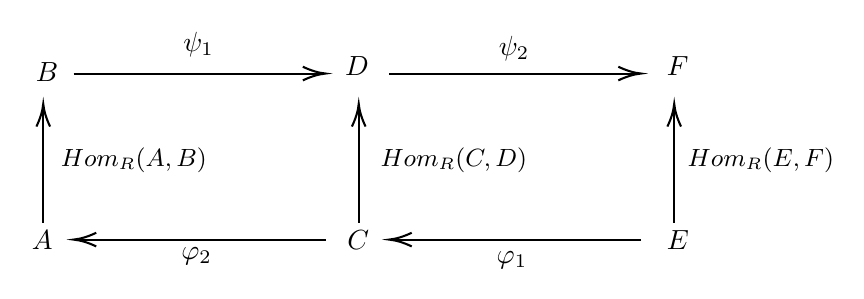
\begin{tikzpicture}[x=0.75pt,y=0.75pt,yscale=-1,xscale=1]
%uncomment if require: \path (0,476); %set diagram left start at 0, and has height of 476

%Straight Lines [id:da2920246208679915] 
\draw    (192,240) -- (192,184.61) ;
\draw [shift={(192,182.61)}, rotate = 90] [color={rgb, 255:red, 0; green, 0; blue, 0 }  ][line width=0.75]    (10.93,-3.29) .. controls (6.95,-1.4) and (3.31,-0.3) .. (0,0) .. controls (3.31,0.3) and (6.95,1.4) .. (10.93,3.29)   ;
%Straight Lines [id:da04506002983020263] 
\draw    (344,240) -- (344,184.61) ;
\draw [shift={(344,182.61)}, rotate = 90] [color={rgb, 255:red, 0; green, 0; blue, 0 }  ][line width=0.75]    (10.93,-3.29) .. controls (6.95,-1.4) and (3.31,-0.3) .. (0,0) .. controls (3.31,0.3) and (6.95,1.4) .. (10.93,3.29)   ;
%Straight Lines [id:da37803238364229985] 
\draw    (206.6,168) -- (326,168) ;
\draw [shift={(328,168)}, rotate = 180] [color={rgb, 255:red, 0; green, 0; blue, 0 }  ][line width=0.75]    (10.93,-3.29) .. controls (6.95,-1.4) and (3.31,-0.3) .. (0,0) .. controls (3.31,0.3) and (6.95,1.4) .. (10.93,3.29)   ;
%Straight Lines [id:da5428498747387094] 
\draw    (328,248) -- (208.6,248) ;
\draw [shift={(206.6,248)}, rotate = 360] [color={rgb, 255:red, 0; green, 0; blue, 0 }  ][line width=0.75]    (10.93,-3.29) .. controls (6.95,-1.4) and (3.31,-0.3) .. (0,0) .. controls (3.31,0.3) and (6.95,1.4) .. (10.93,3.29)   ;
%Straight Lines [id:da0021870933535605985] 
\draw    (358.6,168) -- (478,168) ;
\draw [shift={(480,168)}, rotate = 180] [color={rgb, 255:red, 0; green, 0; blue, 0 }  ][line width=0.75]    (10.93,-3.29) .. controls (6.95,-1.4) and (3.31,-0.3) .. (0,0) .. controls (3.31,0.3) and (6.95,1.4) .. (10.93,3.29)   ;
%Straight Lines [id:da9085135985503727] 
\draw    (480,248) -- (360.6,248) ;
\draw [shift={(358.6,248)}, rotate = 360] [color={rgb, 255:red, 0; green, 0; blue, 0 }  ][line width=0.75]    (10.93,-3.29) .. controls (6.95,-1.4) and (3.31,-0.3) .. (0,0) .. controls (3.31,0.3) and (6.95,1.4) .. (10.93,3.29)   ;
%Straight Lines [id:da06661859833245565] 
\draw    (496,240) -- (496,184.61) ;
\draw [shift={(496,182.61)}, rotate = 90] [color={rgb, 255:red, 0; green, 0; blue, 0 }  ][line width=0.75]    (10.93,-3.29) .. controls (6.95,-1.4) and (3.31,-0.3) .. (0,0) .. controls (3.31,0.3) and (6.95,1.4) .. (10.93,3.29)   ;

% Text Node
\draw (187,161.4) node [anchor=north west][inner sep=0.75pt]    {$B$};
% Text Node
\draw (336,158.4) node [anchor=north west][inner sep=0.75pt]    {$D$};
% Text Node
\draw (185,242.4) node [anchor=north west][inner sep=0.75pt]    {$A$};
% Text Node
\draw (337,242.4) node [anchor=north west][inner sep=0.75pt]    {$C$};
% Text Node
\draw (257,250.4) node [anchor=north west][inner sep=0.75pt]    {$\varphi _{2}$};
% Text Node
\draw (258,146.4) node [anchor=north west][inner sep=0.75pt]    {$\psi _{1}$};
% Text Node
\draw (199,202.4) node [anchor=north west][inner sep=0.75pt]  [font=\small]  {$\text{Hom}_{R}( A,B)$};
% Text Node
\draw (353,202.4) node [anchor=north west][inner sep=0.75pt]  [font=\small]  {$\text{Hom}_{R}( C,D)$};
% Text Node
\draw (491,242.4) node [anchor=north west][inner sep=0.75pt]    {$E$};
% Text Node
\draw (491,158.4) node [anchor=north west][inner sep=0.75pt]    {$F$};
% Text Node
\draw (410,148.4) node [anchor=north west][inner sep=0.75pt]    {$\psi _{2}$};
% Text Node
\draw (409,252.4) node [anchor=north west][inner sep=0.75pt]    {$\varphi _{1}$};
% Text Node
\draw (501,202.4) node [anchor=north west][inner sep=0.75pt]  [font=\small]  {$\text{Hom}_{R}( E,F)$};


\end{tikzpicture}
\end{center}
is as follows: 
$$
\mathrm{Hom}\left( \varphi _1,\psi _2 \right) \mathrm{Hom}\left( \varphi _2,\psi _1 \right) =\mathrm{Hom}\left( \varphi _2\varphi _1,\psi _2\psi _1 \right) :\mathrm{Hom}_R\left( A,B \right) \rightarrow \mathrm{Hom}_R\left( E,F \right) .
$$
There are two special cases of the induced homomorphism. If $B=D$ and $\psi=1_B$, then the induced map $\mathrm{Hom}(\varphi,1_B)$ is given by $f\mapsto f\varphi$ and is denoted $\overline{\varphi}$. Similarly if $A=C$ and $\varphi=1_A$ the induced map $\mathrm{Hom}(1_A,\psi)$ is given by $f\mapsto\psi f$ and is denoted $\overline{\psi}$. The diagram in this case is presented below: 
\begin{center}


\tikzset{every picture/.style={line width=0.75pt}} %set default line width to 0.75pt        

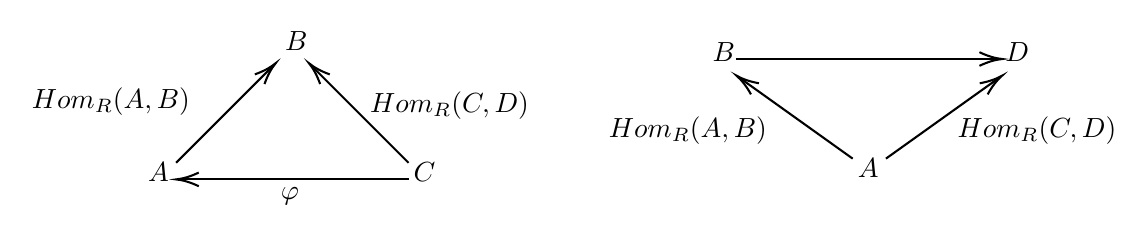
\begin{tikzpicture}[x=0.75pt,y=0.75pt,yscale=-1,xscale=1]
%uncomment if require: \path (0,476); %set diagram left start at 0, and has height of 476

%Straight Lines [id:da597002119082159] 
\draw    (264,235) -- (154,235) ;
\draw [shift={(152,235)}, rotate = 360] [color={rgb, 255:red, 0; green, 0; blue, 0 }  ][line width=0.75]    (10.93,-3.29) .. controls (6.95,-1.4) and (3.31,-0.3) .. (0,0) .. controls (3.31,0.3) and (6.95,1.4) .. (10.93,3.29)   ;
%Straight Lines [id:da1798127284338633] 
\draw    (152,227) -- (198.59,180.41) ;
\draw [shift={(200,179)}, rotate = 135] [color={rgb, 255:red, 0; green, 0; blue, 0 }  ][line width=0.75]    (10.93,-3.29) .. controls (6.95,-1.4) and (3.31,-0.3) .. (0,0) .. controls (3.31,0.3) and (6.95,1.4) .. (10.93,3.29)   ;
%Straight Lines [id:da051057573396247724] 
\draw    (264,227) -- (217.41,180.41) ;
\draw [shift={(216,179)}, rotate = 45] [color={rgb, 255:red, 0; green, 0; blue, 0 }  ][line width=0.75]    (10.93,-3.29) .. controls (6.95,-1.4) and (3.31,-0.3) .. (0,0) .. controls (3.31,0.3) and (6.95,1.4) .. (10.93,3.29)   ;
%Straight Lines [id:da31040695645518945] 
\draw    (478,225) -- (423.63,186.16) ;
\draw [shift={(422,185)}, rotate = 35.54] [color={rgb, 255:red, 0; green, 0; blue, 0 }  ][line width=0.75]    (10.93,-3.29) .. controls (6.95,-1.4) and (3.31,-0.3) .. (0,0) .. controls (3.31,0.3) and (6.95,1.4) .. (10.93,3.29)   ;
%Straight Lines [id:da054410057315041005] 
\draw    (422,177) -- (548,177) ;
\draw [shift={(550,177)}, rotate = 180] [color={rgb, 255:red, 0; green, 0; blue, 0 }  ][line width=0.75]    (10.93,-3.29) .. controls (6.95,-1.4) and (3.31,-0.3) .. (0,0) .. controls (3.31,0.3) and (6.95,1.4) .. (10.93,3.29)   ;
%Straight Lines [id:da5548694030859183] 
\draw    (494,225) -- (548.37,186.16) ;
\draw [shift={(550,185)}, rotate = 144.46] [color={rgb, 255:red, 0; green, 0; blue, 0 }  ][line width=0.75]    (10.93,-3.29) .. controls (6.95,-1.4) and (3.31,-0.3) .. (0,0) .. controls (3.31,0.3) and (6.95,1.4) .. (10.93,3.29)   ;

% Text Node
\draw (137,225.4) node [anchor=north west][inner sep=0.75pt]    {$A$};
% Text Node
\draw (265,225.4) node [anchor=north west][inner sep=0.75pt]    {$C$};
% Text Node
\draw (203,162.4) node [anchor=north west][inner sep=0.75pt]    {$B$};
% Text Node
\draw (201,237.4) node [anchor=north west][inner sep=0.75pt]    {$\varphi $};
% Text Node
\draw (81,189.4) node [anchor=north west][inner sep=0.75pt]    {$\text{Hom}_{R}( A,B)$};
% Text Node
\draw (244,191.4) node [anchor=north west][inner sep=0.75pt]    {$\text{Hom}_{R}( C,D)$};
% Text Node
\draw (479,223.4) node [anchor=north west][inner sep=0.75pt]    {$A$};
% Text Node
\draw (550,167.4) node [anchor=north west][inner sep=0.75pt]    {$D$};
% Text Node
\draw (409,167.4) node [anchor=north west][inner sep=0.75pt]    {$B$};
% Text Node
\draw (359,203.4) node [anchor=north west][inner sep=0.75pt]    {$\text{Hom}_{R}( A,B)$};
% Text Node
\draw (527,203.4) node [anchor=north west][inner sep=0.75pt]    {$\text{Hom}_{R}( C,D)$};


\end{tikzpicture}
\end{center}
We now examine the behavior of $\mathrm{Hom}_R$ with respect to exact sequences.
\begin{theorem}
Let $R$ be a ring. $0\longrightarrow A\overset{\varphi}{\longrightarrow}B\overset{\psi}{\longrightarrow}C$ is an exact sequence of $R$-modules if and only if for every $R$-module $D$ 
$$
0\longrightarrow \mathrm{Hom}_R\left( D,A \right) \overset{\overline{\varphi }}{\longrightarrow}\mathrm{Hom}_R\left( D,B \right) \overset{\overline{\psi }}{\longrightarrow}\mathrm{Hom}_R\left( D,C \right) 
$$
is an exact sequence of abelian groups.
\end{theorem}
\begin{proof}
Suppose $0\longrightarrow A\overset{\varphi}{\longrightarrow}B\overset{\psi}{\longrightarrow}C$ is an exact sequence of $R$-modules, we first show that $\mathrm{Ker}\overline{\varphi}=0$. Let $f\in\mathrm{Ker}\overline{\varphi}$. Then $\varphi f=0$, whence for all $x\in D$ we have $\varphi f(x)=0$. Since $\mathrm{Ker}\varphi=0$, we have $f(x)=0$ for all $x\in D$, whence $f=0$ and hence $\mathrm{Ker}\overline{\varphi}=0$. We next show that $\mathrm{Im}\overline{\varphi}=\mathrm{Ker}\overline{\psi}$. Since $\mathrm{Im}\varphi=\mathrm{Ker}\psi$, we have $\overline{\psi}\overline{\varphi}=\overline{\psi\varphi}=0$, whence $\mathrm{Im}\overline{\varphi}\subset\mathrm{Ker}\overline{\psi}$. For the converse inclusion, we suppose $g\in\mathrm{Ker}\overline{\psi}$. Then $\psi g=0$, whence $\mathrm{Im}g\subset\mathrm{Ker}\psi=\mathrm{Im}\varphi$. Now if $h$ is defined by the following composition: 
$$
D\overset{g}{\longrightarrow}\mathrm{Im}g\overset{\subset}{\longrightarrow}\mathrm{Im}\varphi \overset{\varphi ^{-1}}{\longrightarrow}A,
$$
then $g=\varphi h=\overline{\varphi }\left( h \right) $, whence $g\in\mathrm{Im}\overline{\varphi}$, and hence $\mathrm{Im}\overline{\varphi}=\mathrm{Ker}\overline{\psi}$, whence the sequence 
$$
0\longrightarrow \mathrm{Hom}_R\left( D,A \right) \overset{\overline{\varphi }}{\longrightarrow}\mathrm{Hom}_R\left( D,B \right) \overset{\overline{\psi }}{\longrightarrow}\mathrm{Hom}_R\left( D,C \right) 
$$
is exact.\par
Conversely, assume that the $\mathrm{Hom}$ sequence of induced maps is exact for every $D$. We first show that $\mathrm{Ker}\varphi=0$. Let $D=\mathrm{Ker}\varphi$. Define the inclusion map $i:\ker\varphi\to A$, then $\overline{\varphi}(i)=\varphi i=0$. Since $\mathrm{Ker}\overline{\varphi}=0$, we have $\mathrm{Ker}\varphi=0$. Now let $D=A$. Since $\mathrm{Ker}\overline{\psi}=\mathrm{Im}\overline{\varphi}$, we have $0=\overline{\psi }\overline{\varphi }\left( 1_A \right) =\psi \varphi 1_A=\psi \varphi $, whence $\mathrm{Im}\varphi\subset\mathrm{Ker}\psi$. Finally let $D=\mathrm{Ker}\psi$ and let $j=D\to B$ be the inclusion map. Since $0=\psi j=\overline{\psi}(j)$ and $\mathrm{Ker}\overline{\psi}=\mathrm{Im}\overline{\varphi}$, we have $j=\overline{\varphi}(f)=\varphi f$ for some $f:D\to A$. Therefore for every $x\in D=\mathrm{Ker}\psi$, $x=j(x)=\varphi f(x)\in\mathrm{Im}\varphi$ and $\mathrm{Ker}\psi\subset\mathrm{Im}\varphi$. Thus $\mathrm{Ker}\psi=\mathrm{Im}\varphi$ and hence the sequence $0\longrightarrow A\overset{\varphi}{\longrightarrow}B\overset{\psi}{\longrightarrow}C$ is exact.
\end{proof}
A similar result is as follows: 
\begin{proposition}
Let $R$ be a ring. $A\overset{\theta}{\longrightarrow}B\overset{\xi}{\longrightarrow}C\longrightarrow 0$ is an exact sequence of $R$-modules if and only if for every $R$-module $D$ 
$$
0\longrightarrow \mathrm{Hom}_R\left( C,D \right) \overset{\overline{\xi }}{\longrightarrow}\mathrm{Hom}_R\left( B,D \right) \overset{\overline{\theta }}{\longrightarrow}\mathrm{Hom}_R\left( A,D \right) 
$$
is an exact sequence of abelian groups.
\end{proposition}
The prove of which is similar to that of Theorem 5.36 and we skip the proof of Proposition 5.37. One sometimes summarizes the two preceding results by saying that $\mathrm{Hom}_R(A,B)$ is \textbf{left exact}. It is not true, however, that a short exact sequence $0\longrightarrow A\longrightarrow B\longrightarrow C\longrightarrow 0$ induces a short exact sequence $0\longrightarrow \mathrm{Hom}_R\left( A,D \right) \longrightarrow \mathrm{Hom}_R\left( B,D \right) \longrightarrow \mathrm{Hom}_R\left( C,D \right) \longrightarrow 0$. However the next theorems show that this result does hold in several cases.
\begin{theorem}
The following conditions on modules over a ring $R$ are equivalent.\par
(i) $0\longrightarrow A\overset{\varphi}{\longrightarrow}B\overset{\psi}{\longrightarrow}C\longrightarrow 0$ is a split exact sequence of $R$-modules;\par
(ii) For all $R$-module $D$ we have 
$$
0\longrightarrow \mathrm{Hom}\left( D,A \right) \overset{\overline{\varphi }}{\longrightarrow}\mathrm{Hom}\left( D,B \right) \overset{\overline{\psi }}{\longrightarrow}\mathrm{Hom}\left( D,C \right) \longrightarrow 0
$$
is split exact;\par
(iii) For all $R$-module $D$ we have 
$$
0\longrightarrow \mathrm{Hom}\left( A,D \right) \overset{\overline{\psi }}{\longrightarrow}\mathrm{Hom}\left( B,D \right) \overset{\overline{\varphi }}{\longrightarrow}\mathrm{Hom}\left( C,D \right) \longrightarrow 0
$$
is split exact.
\end{theorem}
\begin{proof}
We only show that (i) and (ii) are equivalent, the equivalence of (i) and (iii) may be proved analogously.\par
Since $0\longrightarrow A\overset{\varphi}{\longrightarrow}B\overset{\psi}{\longrightarrow}C\longrightarrow 0$ is split exact, there exists some $\alpha:B\to A$ such that $\varphi\alpha=1_B$. It is easy to verify that $\overline{\varphi}\overline{\alpha}=1_{\mathrm{Hom}(D,B)}$, whence $\overline{\varphi}$ is an epimorphism. Therefore 
$$
0\longrightarrow \mathrm{Hom}\left( D,A \right) \overset{\overline{\varphi }}{\longrightarrow}\mathrm{Hom}\left( D,B \right) \overset{\overline{\psi }}{\longrightarrow}\mathrm{Hom}\left( D,C \right) \longrightarrow 0
$$
is split exact by Theorem 5.36. Conversely, suppose $D=A$ and $f:B\to A$ is such that $\overline{\varphi}(f)=f\varphi$, then $\varphi$ is a monomorphism, therefore $0\longrightarrow A\overset{\varphi}{\longrightarrow}B\overset{\psi}{\longrightarrow}C\longrightarrow 0$ is split exact by Theorem 5.12 and the proof is finished.
\end{proof}
\begin{theorem}
The following three statements are equivalent:\par
(i) $P$ is projective;\par
(ii) If $\psi:B\to C$ is any $R$-module epimorphism then $\overline{\psi}:\mathrm{Hom}(P,B)\to\mathrm{Hom}(P,C)$ is an epimorphism of abelian groups;\par
(iii) If $0\longrightarrow A\overset{\varphi}{\longrightarrow}B\overset{\psi}{\longrightarrow}C\longrightarrow 0$ is split exact is any short exact sequence of $R$-modules, then 
$$
0\longrightarrow \mathrm{Hom}\left( P,A \right) \overset{\overline{\varphi }}{\longrightarrow}\mathrm{Hom}\left( P,B \right) \overset{\overline{\psi }}{\longrightarrow}\mathrm{Hom}\left( P,C \right) \longrightarrow 0
$$
is an exact sequence of abelian groups.
\end{theorem}
\begin{proof}
We first show that (i) and (ii) are equivalent. Note that $\overline{\psi}$ is projective if and only if for every $R$-module homomorphism $f:P\to C$, there is an $R$-module homomorphism $g$ such that 
\begin{center}


\tikzset{every picture/.style={line width=0.75pt}} %set default line width to 0.75pt        

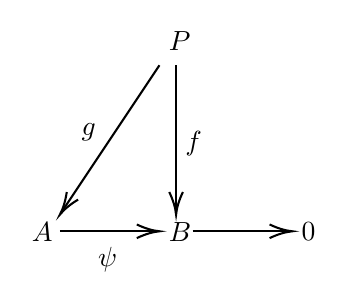
\begin{tikzpicture}[x=0.75pt,y=0.75pt,yscale=-1,xscale=1]
%uncomment if require: \path (0,476); %set diagram left start at 0, and has height of 476

%Straight Lines [id:da28362380995243197] 
\draw    (200,136) -- (200,206) ;
\draw [shift={(200,208)}, rotate = 270] [color={rgb, 255:red, 0; green, 0; blue, 0 }  ][line width=0.75]    (10.93,-3.29) .. controls (6.95,-1.4) and (3.31,-0.3) .. (0,0) .. controls (3.31,0.3) and (6.95,1.4) .. (10.93,3.29)   ;
%Straight Lines [id:da3612305714128048] 
\draw    (144,216) -- (190,216) ;
\draw [shift={(192,216)}, rotate = 180] [color={rgb, 255:red, 0; green, 0; blue, 0 }  ][line width=0.75]    (10.93,-3.29) .. controls (6.95,-1.4) and (3.31,-0.3) .. (0,0) .. controls (3.31,0.3) and (6.95,1.4) .. (10.93,3.29)   ;
%Straight Lines [id:da5138088096735041] 
\draw    (208,216) -- (254,216) ;
\draw [shift={(256,216)}, rotate = 180] [color={rgb, 255:red, 0; green, 0; blue, 0 }  ][line width=0.75]    (10.93,-3.29) .. controls (6.95,-1.4) and (3.31,-0.3) .. (0,0) .. controls (3.31,0.3) and (6.95,1.4) .. (10.93,3.29)   ;
%Straight Lines [id:da29086024261358223] 
\draw    (192,136) -- (145.11,206.34) ;
\draw [shift={(144,208)}, rotate = 303.69] [color={rgb, 255:red, 0; green, 0; blue, 0 }  ][line width=0.75]    (10.93,-3.29) .. controls (6.95,-1.4) and (3.31,-0.3) .. (0,0) .. controls (3.31,0.3) and (6.95,1.4) .. (10.93,3.29)   ;

% Text Node
\draw (195,118.4) node [anchor=north west][inner sep=0.75pt]    {$P$};
% Text Node
\draw (195,210.4) node [anchor=north west][inner sep=0.75pt]    {$B$};
% Text Node
\draw (129,210.4) node [anchor=north west][inner sep=0.75pt]    {$A$};
% Text Node
\draw (259,210.4) node [anchor=north west][inner sep=0.75pt]    {$0$};
% Text Node
\draw (203,166.4) node [anchor=north west][inner sep=0.75pt]    {$f$};
% Text Node
\draw (161,222.4) node [anchor=north west][inner sep=0.75pt]    {$\psi $};
% Text Node
\draw (153,162.4) node [anchor=north west][inner sep=0.75pt]    {$g$};


\end{tikzpicture}
\end{center}
is commutative, whence $P$ is a projective module.\par
Now we show that (ii) and (iii) are equivalent. Suppose $0\longrightarrow A\overset{\varphi}{\longrightarrow}B\overset{\psi}{\longrightarrow}C\longrightarrow 0$, by (ii) we know that $\overline{\psi}$ is an epimorphism, whence 
$$
0\longrightarrow \mathrm{Hom}\left( P,A \right) \overset{\overline{\varphi }}{\longrightarrow}\mathrm{Hom}\left( P,B \right) \overset{\overline{\psi }}{\longrightarrow}\mathrm{Hom}\left( P,C \right) \longrightarrow 0
$$
is an exact sequence of abelian groups by Theorem 5.36. Conversely, consider $A=\mathrm{Ker}\psi$ and the short exact sequence $0\longrightarrow \mathrm{Ker}\psi \overset{\subset}{\longrightarrow}B\overset{\psi}{\longrightarrow}C\longrightarrow 0$, therefore we have 
$$
0\longrightarrow \mathrm{Hom}\left( P,\mathrm{Ker}\psi \right) \overset{\overline{\varphi }}{\longrightarrow}\mathrm{Hom}\left( P,B \right) \overset{\overline{\psi }}{\longrightarrow}\mathrm{Hom}\left( P,C \right) \longrightarrow 0
$$
exact, whence $\overline{\psi}$ is an epimorphism.
\end{proof}
The dual of Theorem 5.39 may be stated as follows: 
\begin{theorem}
The following three statements are equivalent:\par
(i) $J$ is injective;\par
(ii) If $\theta:A\to B$ is any $R$-module monomorphism, then $\overline{\theta}:\mathrm{Hom}(B,J)\to\mathrm{Hom}(A,J)$ is an epimorphism of abelian groups;\par
(iii) If $0\longrightarrow A\overset{\theta}{\longrightarrow}B\overset{\xi}{\longrightarrow}C\longrightarrow 0$ is any short exact sequence of $R$-modules, then 
$$
0\longrightarrow \mathrm{Hom}\left( A,J \right) \overset{\overline{\theta }}{\longrightarrow}\mathrm{Hom}\left( B,J \right) \overset{\overline{\xi }}{\longrightarrow}\mathrm{Hom}\left( C,J \right) \longrightarrow 0
$$
is an exact sequence of abelian groups.
\end{theorem}
The proof of Theorem 5.40 is the dual of Theorem 5.39 and we skip the details.
\begin{theorem}
Let $A,B,\{A_i:i\in I\}$ and $\{B_j:j\in J\}$ be modules over a ring $R$. Then there are isomorphisms of abelian groups:
$$
\mathrm{Hom}\left( \bigoplus_{i\in I}{A_i},B \right) \cong \prod_{i\in I}{\mathrm{Hom}\left( A_i,B \right)};\hspace{0.5cm}\mathrm{Hom}\left( A,\prod_{j\in J}{B_j} \right) \cong \prod_{j\in J}{\mathrm{Hom}\left( A,B_j \right)}.
$$
\end{theorem}
\begin{proof}
We only prove the first isomorphism, and the second one may be proved analogously. Recall the universal property of direct product, we know that for any $\{g_i\}\in\prod\mathrm{Hom}(A_i,B)$, there exists a unique $g\in\mathrm{Hom}\left(\prod A_i,B\right)$ such that the following diagram is commutative: 
\begin{center}


\tikzset{every picture/.style={line width=0.75pt}} %set default line width to 0.75pt        

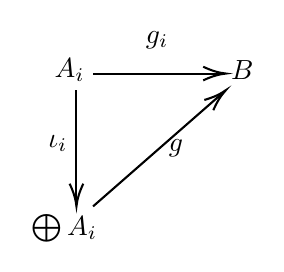
\begin{tikzpicture}[x=0.75pt,y=0.75pt,yscale=-1,xscale=1]
%uncomment if require: \path (0,476); %set diagram left start at 0, and has height of 476

%Straight Lines [id:da8762365885549739] 
\draw    (232,160) -- (294,160) ;
\draw [shift={(296,160)}, rotate = 180] [color={rgb, 255:red, 0; green, 0; blue, 0 }  ][line width=0.75]    (10.93,-3.29) .. controls (6.95,-1.4) and (3.31,-0.3) .. (0,0) .. controls (3.31,0.3) and (6.95,1.4) .. (10.93,3.29)   ;
%Straight Lines [id:da025156901833905287] 
\draw    (224,168) -- (224,222) ;
\draw [shift={(224,224)}, rotate = 270] [color={rgb, 255:red, 0; green, 0; blue, 0 }  ][line width=0.75]    (10.93,-3.29) .. controls (6.95,-1.4) and (3.31,-0.3) .. (0,0) .. controls (3.31,0.3) and (6.95,1.4) .. (10.93,3.29)   ;
%Straight Lines [id:da02970795180480046] 
\draw    (232,224) -- (294.49,169.32) ;
\draw [shift={(296,168)}, rotate = 138.81] [color={rgb, 255:red, 0; green, 0; blue, 0 }  ][line width=0.75]    (10.93,-3.29) .. controls (6.95,-1.4) and (3.31,-0.3) .. (0,0) .. controls (3.31,0.3) and (6.95,1.4) .. (10.93,3.29)   ;

% Text Node
\draw (212,151.4) node [anchor=north west][inner sep=0.75pt]    {$A_{i}$};
% Text Node
\draw (201,226.4) node [anchor=north west][inner sep=0.75pt]    {$\bigoplus A_{i}$};
% Text Node
\draw (297,152.4) node [anchor=north west][inner sep=0.75pt]    {$B$};
% Text Node
\draw (256,138.4) node [anchor=north west][inner sep=0.75pt]    {$g_{i}$};
% Text Node
\draw (209,188.4) node [anchor=north west][inner sep=0.75pt]    {$\iota _{i}$};
% Text Node
\draw (267,190.4) node [anchor=north west][inner sep=0.75pt]    {$g$};


\end{tikzpicture}
\end{center}
whence $g_i=g\iota_i$, where $\iota_i$ is the canonical injection. Define $\psi:\prod\mathrm{Hom}(A_i,B)\to\mathrm{Hom}\left(\bigoplus A_i,B\right)$ to be $\{g_i\}\mapsto g$and $\varphi:\mathrm{Hom}\left(\bigoplus A_i,B\right)\to\prod\mathrm{Hom}(A_i,B)$ to be $f\mapsto\{f\iota_i\}$, then it is easy to verify that $\psi$ and $\varphi$ are homomorphisms, and $\varphi\psi=1_{\prod\mathrm{Hom}(A_i,B)}$, $\psi\varphi=1_{\mathrm{Hom}\left(\bigoplus A_i,B\right)}$. Therefore $\varphi$ and $\psi$ are isomorphisms, and hence $\mathrm{Hom}\left(\bigoplus A_i,B\right)\cong\prod\mathrm{Hom}(A_i,B)$.
\end{proof}
In order to deal with duality and other concepts we need to consider possible module structures on the abelian group $\mathrm{Hom}_R(A,B)$. We begin with some remarks about bimodules. Let $R$ and $S$ be rings. An abelian group $A$ is an $R-S$ \textbf{bimodule} if $A$ is a left $R$-module and a right $S$-module, and $(ra)s=r(as)$ for all $r\in R$, $s\in S$ and $a\in A$. We shall denote an $R-S$ bimodule by $_RA_S$. Sometimes we write $_RB$ and $C_S$ to indicate that $B$ is a left $R$-module and $C$ is a right $S$-module.\par
\begin{theorem}
Let $R$ and $S$ be rings and let $_RA$, $_RB_S$, $_RC_S$ and $_RD$ be (bi)modules as indicated.\par
(i) $\mathrm{Hom}_R(A,B)$ is a right $S$-module, with the action of $S$ given by $(fs)(a)=f(a)s$, where $f\in\mathrm{Hom}_R(A,B)$, $s\in S$ and $a\in A$.\par
(ii) If $\varphi:A\to A^\prime$ is a homomorphism of left $R$-modules, then the induced map $\overline{\varphi}:\mathrm{Hom}_R(A^\prime,B)\to\mathrm{Hom}_R(A,B)$ is a homomorphism of $S$-modules.\par
(iii) $\mathrm{Hom}_R(C,D)$ is a left $S$-module, with the action of $S$ given by $(sg)(c)=g(cs)$, where $g\in\mathrm{Hom}_R(C,D)$, $s\in S$ and $c\in C$.\par
(iv) If $\psi:D\to D^\prime$ is a homomorphism of left $R$-modules, then $\overline{\psi}:\mathrm{Hom}_R(C,D)\to\mathrm{Hom}_R(C,D^\prime)$ is a homomorphism of left $S$-modules.
\end{theorem}
\begin{proof}
(i) and (iii) follows directly from definition. We prove the latter part of  (i) only. Suppose $f,g\in\mathrm{Hom}_R(A,B)$ and $s,t\in S$. Then 
$$
\left[ \left( f+g \right) s \right] \left( a \right) =\left( f+g \right) \left( a \right) s=\left[ f\left( a \right) +g\left( a \right) \right] s=f\left( a \right) s+g\left( a \right) s=\left( fs \right) \left( a \right) +\left( gs \right) \left( a \right) ,
$$
and 
$$
f\left( s+t \right) \left( a \right) =f\left( a \right) \left( s+t \right) =f\left( a \right) s+f\left( a \right) t=\left( fs \right) \left( a \right) +\left( ft \right) \left( a \right) ,
$$
and 
$$
\left[ \left( fs \right) t \right] \left( a \right) =\left( fs \right) \left( a \right) t=f\left( a \right) st=\left[ f\left( st \right) \right] \left( a \right) ,
$$
which implies that $\mathrm{Hom}_R(A,B)$ is a right $S$-module.\par
We now prove (ii). Theorem 5.35 states that $\overline{\varphi}$ is an abelian group homomorphism. We now show that it is actually a module homomorphism. Note that 
$$
\overline{\varphi }\left( fs \right) \left( a \right) =\left[ \left( fs \right) \varphi \right] \left( a \right) =\left( fs \right) \left[ \varphi \left( a \right) \right] =\left[ f\left( \varphi \left( a \right) \right) \right] \left( s \right) =\left[ \overline{\varphi }f\left( a \right) \right] s,
$$
hence $\overline{\varphi }\left( fs \right) =\left( \overline{\varphi }f \right) s$ and $\overline{\varphi}$ a homomorphism of right $S$-modules. (iv) is proved in an analogous way.
\end{proof}
\begin{note}\em
A special case of Theorem 5.42 is when $R$ is commutative and hence every $R$-module $C$ is an $R-R$ bimodule with $rc=cr$, where $r\in R$ and $c\in C$. In this case for every $r\in R$, $a\in A$ and $f\in\mathrm{Hom}_R(A,B)$ we have $(rf)(a)=(fr)(a)$, hence $\mathrm{Hom}_R(A,B)$ is an $R-R$ bimodule with $rf=fr$ for all $r\in R$ and $f\in\mathrm{Hom}_R(A,B)$.
\end{note}
\begin{theorem}
Let $A$ be a unitary left module over a ring $R$ with identity. Then there is an isomorphism of left $R$-modules $A\cong\mathrm{Hom}_R(R,A)$.
\end{theorem}
\begin{proof}
Since $R$ is an $R-R$ module, Theorem 5.42 (iii) shows that $\mathrm{Hom}_R(R,A)$ is a left $R$-module. Now define $\varphi:\mathrm{Hom}_R(R,A)\to A$ given by $f\mapsto f(1_R)$, we show that $\varphi$ is an $R$-module homomorphism. First note that 
$$
\varphi \left( fg \right) =\left( fg \right) \left( 1_R \right) =f\left( 1_R \right) g\left( 1_R \right) =\varphi \left( f \right) \varphi \left( g \right) ,
$$
we have $\varphi$ a homomorphism of abelian groups. Then note that 
$$
\varphi \left( rf \right) =rf\left( 1_R \right) =r\varphi \left( f \right) 
$$
for all $r\in R$ and $f\in\mathrm{Hom}_R(R,A)$, we have $\varphi$ an $R$-module homomorphism. Next we define $\psi:A\to\mathrm{Hom}_R(R,A)$ given by $a\mapsto f_a$, where $f_a(r)=ra$ for all $r\in R$. Then $\psi$ is also a homomorphism of $R$-modules. Note that 
$$
\psi \left( ab \right) =f_{ab}=f_af_b,
$$
where the last equality follows from the fact 
$$
f_{ab}\left( r \right) =rab;f_af_b\left( r \right) =f_a\left( rb \right) =rba=rab,
$$
we have $\psi$ an abelian group homomorphism. Next we observe that 
$$
\psi \left( ra \right) =f_{ra}=rf_a,
$$
where the last equality follows from the fact 
$$
f_{ra}\left( s \right) =sra;\left( rf_a \right) \left( s \right) =f_a\left( sr \right) =sra,
$$
we have $\psi$ an $R$-module homomorphism. Now observe that 
$$
\varphi \psi \left( a \right) =\varphi \left( f_a \right) =f_a\left( 1_R \right) =1_Ra=a
$$
and 
$$
\psi \varphi \left( f \right) \left( a \right) =\psi \left( f\left( 1_R \right) \right) \left( a \right) =f_{f\left( 1_R \right)}\left( a \right) =af\left( 1_R \right) =a,
$$
we have $\varphi\psi=1_A$ and $\psi\varphi=1_{\mathrm{Hom}_R(R,A)}$, therefore $\varphi$ is an isomorphism of $R$-modules, hence $A\cong\mathrm{Hom}_R(R,A)$.
\end{proof}
Let $A$ be a left module over a ring $R$. Since $R$ is an $R-R$ module, $\mathrm{Hom}_R(A,R)$ is a right $R$-module by Theorem 5.44 (i). $\mathrm{Hom}_R(A,R)$ is called the \textbf{dual} module of $A$ and is denoted by $A^*$. The elements of $A^*$ are sometimes called \textbf{linear functionals}. Similarly if $B$ is a right $R$-module, then the dual $B^*$ of $B$ is a left $R$-module $\mathrm{Hom}_R(B,R)$.
\begin{theorem}
Let $A,B$ and $C$ be left modules over a ring $R$.\par
(i) If $\varphi:A\to C$ is a homomorphism of left $R$-modules, then the induced map $\overline{\varphi}:C^*\to A^*$ is a homomorphism of right $R$-modules.\par
(ii) There is an $R$-module isomorphism $\left( A\oplus B \right) ^*\cong A^*\oplus B^*$.\par
(iii) If $R$ is a division ring and $0\longrightarrow A\overset{\theta}{\longrightarrow}B\overset{\xi}{\longrightarrow}C\longrightarrow 0$ is a short exact sequence of left vector spaces, then $0\longrightarrow C^*\overset{\overline{\xi }}{\longrightarrow}B^*\overset{\overline{\theta }}{\longrightarrow}A^*\longrightarrow 0$ is a short exact sequence of right vector spaces.
\end{theorem}
\begin{proof}
(i) See Theorem 5.35.\par
(ii) By Theorem 5.41 we have 
$$
\left( A\oplus B \right) ^*=\mathrm{Hom}_R\left( A\oplus B,R \right) \cong \mathrm{Hom}_R\left( A,R \right) \times \mathrm{Hom}_R\left( B,R \right) =A^*\oplus B^*,
$$
whence $\left( A\oplus B \right) ^*\cong A^*\oplus B^*$.\par
(iii) By Exercise 5.28 we know that $R$ is injective over $R$, therefore by Theorem 5.40 we know that 
$$
0\longrightarrow \mathrm{Hom}_R\left( C,R \right) \overset{\overline{\xi }}{\longrightarrow}\mathrm{Hom}_R\left( B,R \right) \overset{\overline{\theta }}{\longrightarrow}\mathrm{Hom}_R\left( A,R \right) \longrightarrow 0
$$
is short exact, whence $0\longrightarrow C^*\overset{\overline{\xi }}{\longrightarrow}B^*\overset{\overline{\theta }}{\longrightarrow}A^*\longrightarrow 0$ is a short exact sequence of right vector spaces.
\end{proof}
If $A$ is a left module over a ring $R$, $a\in A$, and $f\in A^*=\mathrm{Hom}_R(A,R)$, then one frequently denotes $f(a)\in R$ by $\left<a,f\right>$. Since $f$ is a left $R$-module homomorphism, we have 
$$
\left< r_1a_1+r_2a_2,f \right> =f\left( r_1a_1+r_2a_2 \right) =r_1f\left( a_1 \right) +r_2f\left( a_2 \right) =r_1\left< a_1,f \right> +r_2\left< a_2,f \right> 
$$
and 
$$
\left< a,f_1r_1+f_2r_2 \right> =\left( f_1r_1+f_2r_2 \right) \left( a \right) =f_1\left( a \right) r_1+f_2\left( a \right) r_2=\left< a,f_1 \right> r_1+\left< a,f_2 \right> r_2
$$
for all $a_1,a_2,a\in A$, $f_1,f_2,f\in A^*$ and $r_1,r_2\in R$.\par
In order to simplify our notations, we shall introduce the \textbf{Kronecker delta notation}: for any index set $I$ and ring $R$ with identity the symbol $\delta_{ij}$ ($i,j\in I$) denotes $0\in R$ if $i\ne j$ and $1_R\in R$ if $i=j$.
\begin{theorem}
Let $F$ be a free left module over a ring $R$ with identity. Let $X$ be a basis of $F$ and for each $x\in X$ let $f_x:F\to R$ be given by $f_x(y)=\delta_{xy}$ for $y\in X$. Then \par
(i) $\{f_x:x\in X\}$ is a linearly independent subset of $F^*$ of cardinality $|X|$;\par
(ii) If $X$ is finite, then $F^*$ is a free right $R$-module with basis $\{f_x:x\in X\}$.
\end{theorem}
\begin{proof}
(i) We first show that $\{f_x\}$ is linearly independent. Suppose $f_{x_1}r_1+f_{x_2}r_2+\cdots +f_{x_n}r_n=0$, then 
$$
0=\left< x_j,0 \right> =\left< x_j,\sum_{i=1}^n{f_{x_i}r_i} \right> =\sum_{i=1}^n{\left< x_j,f_{x_i} \right> r_i}=\sum_{i=1}^n{\delta _{ij}r_i}=r_j,
$$
whence $r_j=0$ for all $j=1,2,\cdots,n$, therefore $\{f_x\}$ is linearly independent. Now suppose $x\ne y\in X$, then $f_x(x)=1_R\ne 0=f_x(y)$, therefore $f_x\ne f_y$ and hence $\{f_x\}$ has cardinality $|X|$.\par
(ii) Since $X$ is finite, let $X=\{x_1,x_2,\cdots,x_n\}$ and denote $f_{x_i}$ as $f_i$. Suppose $f\in F^*$ and $s_i=f(x_i)=\left<x_i,f\right>$. Let $u=r_1x_1+r_2x_2+\cdots+r_nx_n\in F$, observe that 
$$
\begin{aligned}
\left< u,\sum_{j=1}^n{f_js_j} \right> &=\left< \sum_{i=1}^n{r_ix_i},\sum_{j=1}^n{f_js_j} \right> =\sum_{i=1}^n{\sum_{j=1}^n{r_i\left< x_i,f_j \right> s_j}}=\sum_{i=1}^n{\sum_{j=1}^n{r_i\delta _{ij}s_j}}
\\
&=\sum_{i=1}^n{r_is_i}=\sum_{i=1}^n{r_i\left< x_i,f \right>}=\left< \sum_{i=1}^n{r_ix_i},f \right> =\left< u,f \right> ,
\end{aligned}
$$
we have $f=f_1s_1+f_2s_2+\cdots+f_ns_n$, and hence $\{f_i\}$ generated $F^*$. Hence $\{f_i\}$ is a basis of the free module $F^*$.
\end{proof}
\begin{note}\em
The homomorphisms $f_x$ are well-defined since $F$ is free with basis $X$. $\{f_x:x\in X\}$ is called the \textbf{dual basis} to $X$. Note that if $F$ is finite dimensional and $R$ has invariance dimension property, then $F\cong F^*$ since there bases have the same cardinality. In particular, this is true when $F$ is a vector space of finite dimension.
\end{note}
The process of forming duals may be repeated. If $A$ is a left $R$-module, then $A^*$ id a ring $R$-module and $A^{**}=(A^*)^*=\mathrm{Hom}_R(\mathrm{Hom}_R(A,R)R)$ is a left $R$-module. $A^{**}$ is called the \textbf{double dual} of $A$. 
\begin{theorem}
Let $A$ be a left module over a ring $R$.\par
(i) There is an $R$-module homomorphism $\theta:A\to A^{**}$.\par
(ii) If $R$ has an identity and $A$ is a free module over $R$, then $\theta$ is a monomorphism.\par
(iii) If $R$ has an identity and $A$ is a free module over $R$ of finite rank, then $A\cong A^{**}$.
\end{theorem}
\begin{proof}
(i) Let $a\in A$ and we define $\theta_a:A^*\to R$ to be $f\mapsto\left<a,f\right>$. Then $\theta:a\mapsto\theta_a$ is easily verified to satisfy the conditions.\par
(ii) Let $X$ be the basis of $A$. If $a\in A$ and $a=r_1x_1+r_2x_2+\cdots+r_nx_n$, where $r_i\in R$ and $x_i\in X$. If $\theta_a(f)=0$, then 
$$
0=\left< a,f \right> =\left< \sum_{i=1}^n{r_ix_i},f \right> =\sum_{i=1}^n{r_i\left< x_i,f \right>}.
$$
In particular, take $f=f_{x_j}$, we have 
$$
0=\sum_{i=1}^n{r_i\left< x_i,f_{x_j} \right>}=\sum_{i=1}^n{r_i\delta _{ij}}=r_j,
$$
whence $a=0$ and hence $\mathrm{Ker}\theta=0$, which implies $\theta$ a monomorphism.\par
(iii) Since $X$ is finite we have $A^*\cong A$. Note that $A^*$ is also a free module with finite basis, therefore $A^{**}\cong A^*$ and hence $A\cong A^{**}$.
\end{proof}
\begin{note}\em
A module $A$ such that $A^{**}\cong A$ is said to be \textbf{reflexive}.
\end{note}
\begin{center}
\begin{large}
    \textbf{Exercises for 5.4}
\end{large}
\end{center}
Note: $R$ is a ring.
\begin{problem}\em
(a) For any abelian group $A$ and positive integer $m$, $\mathrm{Hom}(\mathbb{Z}_m,A)\cong A[m]=\{a\in A:ma=0\}$.\par
(b) $\mathrm{Hom}(\mathbb{Z}_m,\mathbb{Z}_n)\cong\mathbb{Z}_{(m,n)}$.\par
(c) The $\mathbb{Z}$-module $\mathbb{Z}_m$ has $\mathbb{Z}_m^*=0$.\par
(d) For each $k\ge 1$, we have $\mathbb{Z}_m$ a $\mathbb{Z}_{mk}$-module, as a $\mathbb{Z}_{mk}$-module $\mathbb{Z}_m^*\cong\mathbb{Z}_m$.
\end{problem}
\begin{proof}
(a) For each $a\in A$ define $\psi_a:k\mapsto ka$. Then it is easy to verify $\psi$ is a homomorphism from $\mathbb{Z}_m$ to $A$. Now we define $f:\psi_a\mapsto a$, then $f:\mathrm{Hom}(\mathbb{Z}_m,A)\to A[m]$ is a homomorphism of modules. It is easy to verify that $f$ is both injective and surjective, and hence $\mathrm{Hom}(\mathbb{Z}_m,A)\cong A[m]$.\par
(b) By (a) we have 
$$
\mathrm{Hom}\left( \mathbb{Z} _m,\mathbb{Z} _n \right) \cong \mathbb{Z} _m\left[ n \right] \cong \mathbb{Z} _{\left( m,n \right)}.
$$
Therefore $\mathrm{Hom}(\mathbb{Z}_m,\mathbb{Z}_n)\cong\mathbb{Z}_{(m,n)}$.\par
(c) Since $\mathbb{Z}_m$ is a $\mathbb{Z}$-module, then 
$$
\mathbb{Z} _{m}^{*}=\mathrm{Hom}_{\mathbb{Z}}\left( \mathbb{Z} _m,\mathbb{Z} \right) \cong \mathbb{Z} \left[ m \right] =0,
$$
whence $\mathbb{Z}_m^*=0$.\par
(d) Since $\mathbb{Z}_m$ is a $\mathbb{Z}_{mk}$-module, then 
$$
\mathbb{Z} _{m}^{*}=\mathrm{Hom}_{\mathbb{Z} _{mk}}\left( \mathbb{Z} _m,\mathbb{Z} _{mk} \right) \cong \mathbb{Z} _{\left( m,mk \right)}=\mathbb{Z} _m,
$$
whence $\mathbb{Z}_m^*\cong\mathbb{Z}$.
\end{proof}
\begin{problem}\em
If $A$ and $B$ are abelian groups and $m$ and $n$ integers such that $mA=nB=0$, then every element of $\mathrm{Hom}(A,B)$ has order dividing $(m,n)$.
\end{problem}
\begin{proof}
Suppose $f\in\mathrm{Hom}(A,B)$. Then observe that $f(ma)=f(0)=0$ and $f(na)=nf(a)=0$, hence $f$ is of finite order and the order of $f$ divides $(m,n)$.
\end{proof}
\begin{problem}\em
Let $\pi:\mathbb{Z}\to\mathbb{Z}_2$ be the canonical epimorphism. The induced map $\overline{\pi}:\mathrm{Hom}(\mathbb{Z}_2,\mathbb{Z})\to\mathrm{Hom}(\mathbb{Z}_2,\mathbb{Z}_2)$ is the zero map.
\end{problem}
\begin{proof}
We prove that $\mathrm{Hom}(\mathbb{Z}_2,\mathbb{Z})=0$. By Exercise 5.36 we have $\mathrm{Hom}(\mathbb{Z}_2,\mathbb{Z})\cong\mathbb{Z}[2]=0$, hence $\mathrm{Hom}(\mathbb{Z}_2,\mathbb{Z})=0$ and therefore $\overline{\pi}$ is the zero map.
\end{proof}
\begin{problem}\em
Let $R$ be the ring with identity, then there is a ring isomorphism $\mathrm{Hom}_R(R,R)\cong R^{\mathrm{op}}$ where $\mathrm{Hom}_R$ denotes left $R$-module homomorphisms. In particular if $R$ is commutative, we have $\mathrm{Hom}_R(R,R)\cong R$.
\end{problem}
\begin{proof}
We first show that $\mathrm{Hom}_R(R,R)\cong R^{\mathrm{op}}$. For each $a\in R$, define $\psi_a:x\mapsto xa$, then it is easy to verify that there is a one-to-one correspondence between $\psi_a$ and $a$ with $\psi_a\circ\psi_b$ maps $x$ to $xba$ and hence $f:\psi_a\mapsto a$ is a ring isomorphism. Therefore $\mathrm{Hom}_R(R,R)\cong R^{\mathrm{op}}$. Now if $R$ is commutative, then $R^{\mathrm{op}}\cong R$, and hence $\mathrm{Hom}_R(R,R)\cong R$.
\end{proof}
\begin{problem}\em
Let $S$ be a nonempty subset of a vector space $V$ over a division ring. The \textbf{annihilator} of $S$ is the subset $S^0$ of $V^*$ given by $S^0=\{f\in V*:\left<s,f\right>=0\ \text{for all}\ s\in S\}$.\par
(a) $0^0=V^*$ and $V^0=0$. If $S\ne \{0\}$ then $S^0\ne V^*$.\par
(b) If $W$ is a subspace of $V$, then $W^0$ is a subspace of $V^*$.\par
(c) If $W$ is a subspace of $V$ and $V$ has finite dimension, then $\mathrm{dim}W^0=\mathrm{dim}V-\mathrm{dim}W$.\par
(d) Let $W,V$ be as in (c). There is an isomorphism $W^*\cong V^*/W^0$.\par
(e) Let $W,V$ be as in (c). Identify $V^{**}$ as $V$, then $(W^0)^0=W\subset V$.
\end{problem}
\begin{proof}
(a) By definition we have 
$$
0^0=\left\{ f\in V^*:\left< 0,f \right> =0 \right\} =V^*;V^0=\left\{ f\in V^*:\left< s,f \right> =0,\forall s\in V \right\} =\left\{ 0 \right\} .
$$
Now suppose $S\ne\{0\}$. Then there exists some $s\in S$. Since $1_{V^*}$ maps $s$ to $s$, then $1_{V^*}\notin S^0$, hence $S^0\ne V^*$.\par
(b) Suppose $f_1,f_2\in W^0$ and $r_1,r_2\in R$. Fix $s\in W$. Then 
$$
\left< s,f_1r_1+f_2r_2 \right> =\left< s,f_1 \right> r_1+\left< s,f_2 \right> r_2=0,
$$
hence $f_1r_1+f_2r_2\in W^0$ and $W^0$ a subspace of $V^*$.\par
(c) Suppose the basis of $V$ is $\{e_1,e_2,\cdots,e_n\}$. Then $\{e_1^*,e_2^*,\cdots,e_n^*\}$ is the dual basis of $V^*$. Suppose $W$ is a subspace of $V$ with basis $\{e_1,e_2,\cdots,e_t\}$ with $t\le n$. Suppose $s=r_1e_1+\cdots+r_te_t$ with each $r_i\ne 0$ and $f\in W^0$. Note that 
$$
\left< s,f \right> =\left< \sum_{i=1}^t{r_ie_i,f} \right> =\sum_{i=1}^t{r_i\left< e_i,f \right>}=0,
$$
therefore $\left<e_i,f\right>=0$. Now we show that $\{e_{t+1}^*,\cdots,e_n^*\}$ is the basis of $W^0$. Suppose $r_j=f(e_j)$, then 
$$
\left< e_j,f \right> =\left< e_j,\sum_{i=t+1}^n{e_{i}^{*}r_i} \right> =\sum_{i=t+1}^n{\left< e_j,e_{i}^{*} \right> r_i}=\sum_{i=t+1}^n{\delta _{ji}r_i}=r_j,
$$
whence $f=r_{t+1}r_{t+1}^*+\cdots+r_ne_n^*$. Therefore $W^0$ has a basis $\{e_{t+1}^*,\cdots,e_n^*\}$ and hence $\mathrm{dim}W^0=\mathrm{dim}V-\mathrm{dim}W$.\par
(d) We consider the dimension. Since $W$ and $V$ are of finite dimension here, we have 
$$
\mathrm{dim}W^*=\mathrm{dim}W=t=n-\left( n-t \right) =\mathrm{dim}V-\mathrm{dim}W^0=\mathrm{dim}V/W^0,
$$
whence $W^*\cong V/W^0$.\par
(e) By (c) we have $\mathrm{dim}W+\mathrm{dim}W^*=\mathrm{dim}V$. By taking the dual, we have $\mathrm{dim}W^0+\mathrm{dim}(W^0)^0=\mathrm{dim}V^*$. Note that $V\cong V^*$, we have $\mathrm{dim}W=\mathrm{dim}(W^0)^0$ and hence $(W^0)^0\cong W\subset V$.
\end{proof}
\begin{problem}\em
For any homomorphism $f:A\to B$ of left $R$-modules the diagram 
\begin{center}


\tikzset{every picture/.style={line width=0.75pt}} %set default line width to 0.75pt        

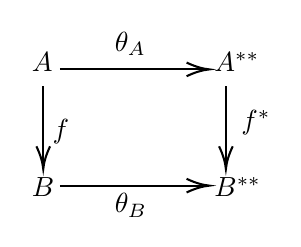
\begin{tikzpicture}[x=0.75pt,y=0.75pt,yscale=-1,xscale=1]
%uncomment if require: \path (0,476); %set diagram left start at 0, and has height of 476

%Straight Lines [id:da5121181270813071] 
\draw    (232,168) -- (302,168) ;
\draw [shift={(304,168)}, rotate = 180] [color={rgb, 255:red, 0; green, 0; blue, 0 }  ][line width=0.75]    (10.93,-3.29) .. controls (6.95,-1.4) and (3.31,-0.3) .. (0,0) .. controls (3.31,0.3) and (6.95,1.4) .. (10.93,3.29)   ;
%Straight Lines [id:da5767169189450072] 
\draw    (232,224) -- (302,224) ;
\draw [shift={(304,224)}, rotate = 180] [color={rgb, 255:red, 0; green, 0; blue, 0 }  ][line width=0.75]    (10.93,-3.29) .. controls (6.95,-1.4) and (3.31,-0.3) .. (0,0) .. controls (3.31,0.3) and (6.95,1.4) .. (10.93,3.29)   ;
%Straight Lines [id:da31437669798313483] 
\draw    (224,176) -- (224,214) ;
\draw [shift={(224,216)}, rotate = 270] [color={rgb, 255:red, 0; green, 0; blue, 0 }  ][line width=0.75]    (10.93,-3.29) .. controls (6.95,-1.4) and (3.31,-0.3) .. (0,0) .. controls (3.31,0.3) and (6.95,1.4) .. (10.93,3.29)   ;
%Straight Lines [id:da4207444628111343] 
\draw    (312,176) -- (312,214) ;
\draw [shift={(312,216)}, rotate = 270] [color={rgb, 255:red, 0; green, 0; blue, 0 }  ][line width=0.75]    (10.93,-3.29) .. controls (6.95,-1.4) and (3.31,-0.3) .. (0,0) .. controls (3.31,0.3) and (6.95,1.4) .. (10.93,3.29)   ;

% Text Node
\draw (217,158.4) node [anchor=north west][inner sep=0.75pt]    {$A$};
% Text Node
\draw (305,158.4) node [anchor=north west][inner sep=0.75pt]    {$A^{**}$};
% Text Node
\draw (217,218.4) node [anchor=north west][inner sep=0.75pt]    {$B$};
% Text Node
\draw (305,218.4) node [anchor=north west][inner sep=0.75pt]    {$B^{**}$};
% Text Node
\draw (257,148.4) node [anchor=north west][inner sep=0.75pt]    {$\theta _{A}$};
% Text Node
\draw (257,226.4) node [anchor=north west][inner sep=0.75pt]    {$\theta _{B}$};
% Text Node
\draw (318,186.4) node [anchor=north west][inner sep=0.75pt]    {$f^{*}$};
% Text Node
\draw (227,190.4) node [anchor=north west][inner sep=0.75pt]    {$f$};


\end{tikzpicture}
\end{center}
is commutative, where $\theta_A$, $\theta_B$ are as theorem 5.46 and $f^*$ is the map induced on $A^{**}=\mathrm{Hom}_R(\mathrm{Hom}_R(A,R),R)$ by the map $\overline{f}:\mathrm{Hom}_R(B,R)\to\mathrm{Hom}_R(A,R)$.
\end{problem}
\begin{proof}
We show that $f^*\theta_A=\theta_Bf$. 
\end{proof}
\begin{problem}\em
Let $F=\bigoplus_{x\in X}\mathbb{Z}x$ be a free $\mathbb{Z}$-module with an infinite basis $X$. Then $\{f_x\}_{x\in X}$ does not form a basis of $F^*$.
\end{problem}
\begin{proof}
Observe that 
$$
F^*=\mathrm{Hom}\left( \bigoplus_{x\in X}{\mathbb{Z} x},\mathbb{Z} \right) \cong \prod_{x\in X}{\mathrm{Hom}\left( \mathbb{Z} x,\mathbb{Z} \right)}\cong \prod_{x\in X}{\mathbb{Z} x}.
$$
However, under this isomorphism $f_y\mapsto\{\delta_{xy}x\}\in\prod_{x\in X}\mathbb{Z}x$, a contradiction!
\end{proof}
\begin{problem}\em
If $R$ has an identity and $P$ is a finitely generated projective unitary $R$-module. Then \par
(a) $P^*$ is a finitely generated projective right module.\par
(b) $P$ is reflexive.
\end{problem}
\begin{proof}
(a) Suppose $P$ is a finitely generated projective module, then $P\cong\bigoplus\mathbb{Z}$ for a finite number of $\mathbb{Z}$. Therefore the dual of $P$ is as follows: 
$$
P^*=\mathrm{Hom}\left( \bigoplus{\mathbb{Z}},\mathbb{Z} \right) \cong \bigoplus{\mathrm{Hom}\left( \mathbb{Z} ,\mathbb{Z} \right)}\cong \bigoplus{\mathbb{Z}}.
$$
Therefore $P^*$ is a finitely generated projective right module.\par
(b) Note that 
$$
P^{**}=\mathrm{Hom}\left( \mathbb{Z} ,\bigoplus{\mathbb{Z}} \right) \cong \bigoplus{\mathrm{Hom}\left( \mathbb{Z} ,\mathbb{Z} \right)}\cong \bigoplus{\mathbb{Z}}=P,
$$
we proved that $P\cong P^{**}$.
\end{proof}
\subsection{Tensor Products}
The tensor product $A\otimes_R B$ of modules $A_R$ and $_RB$ over a ring $R$ is a certain abelian group, which plays an important role in the study of multilinear algebra. We first give the definition of a middle linear map.
\begin{definition}
If $A_R$ and $_RB$ are modules over a ring $R$, and $C$ is an (additive) abelian group, then a \textbf{middle linear map} from $A\times B$ to $C$ is a function $f:A\times B\to C$ such that for all $a,a_i\in A$, $b,b_i\in B$ and $r\in R$: 
$$
f\left( a_1+a_2,b \right) =f\left( a_1,b \right) +f\left( a_2,b \right) ;
$$
$$
f\left( a,b_1+b_2 \right) =f\left( a,b_1 \right) +f\left( a,b_2 \right) ;
$$
$$
f\left( ar,b \right) =f\left( a,rb \right) .
$$
\end{definition}
For fixed $A_R,_RB$ consider the category $\mathfrak{M}(A,B)$ whose objects are all middle linear maps on $A\times B$. By definition a morphism in $\mathfrak{M}(A,B)$ from the middle linear map $f:A\times B\to C$ to the middle linear map $g:A\times B\to D$ is a group homomorphism $h:C\to D$ such that the diagram 
\begin{center}


\tikzset{every picture/.style={line width=0.75pt}} %set default line width to 0.75pt        

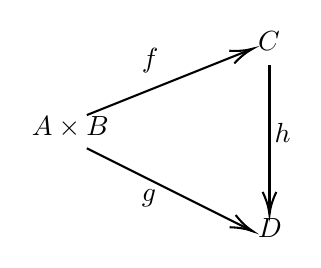
\begin{tikzpicture}[x=0.75pt,y=0.75pt,yscale=-1,xscale=1]
%uncomment if require: \path (0,476); %set diagram left start at 0, and has height of 476

%Straight Lines [id:da4195790388976812] 
\draw    (248,184) -- (326.14,152.74) ;
\draw [shift={(328,152)}, rotate = 158.2] [color={rgb, 255:red, 0; green, 0; blue, 0 }  ][line width=0.75]    (10.93,-3.29) .. controls (6.95,-1.4) and (3.31,-0.3) .. (0,0) .. controls (3.31,0.3) and (6.95,1.4) .. (10.93,3.29)   ;
%Straight Lines [id:da12067463791682087] 
\draw    (248,200) -- (326.21,239.11) ;
\draw [shift={(328,240)}, rotate = 206.57] [color={rgb, 255:red, 0; green, 0; blue, 0 }  ][line width=0.75]    (10.93,-3.29) .. controls (6.95,-1.4) and (3.31,-0.3) .. (0,0) .. controls (3.31,0.3) and (6.95,1.4) .. (10.93,3.29)   ;
%Straight Lines [id:da47119305107127274] 
\draw    (336,160) -- (336,230) ;
\draw [shift={(336,232)}, rotate = 270] [color={rgb, 255:red, 0; green, 0; blue, 0 }  ][line width=0.75]    (10.93,-3.29) .. controls (6.95,-1.4) and (3.31,-0.3) .. (0,0) .. controls (3.31,0.3) and (6.95,1.4) .. (10.93,3.29)   ;

% Text Node
\draw (220,183.4) node [anchor=north west][inner sep=0.75pt]    {$A\times B$};
% Text Node
\draw (329,142.4) node [anchor=north west][inner sep=0.75pt]    {$C$};
% Text Node
\draw (329,232.4) node [anchor=north west][inner sep=0.75pt]    {$D$};
% Text Node
\draw (273,150.4) node [anchor=north west][inner sep=0.75pt]    {$f$};
% Text Node
\draw (273,218.4) node [anchor=north west][inner sep=0.75pt]    {$g$};
% Text Node
\draw (337,186.4) node [anchor=north west][inner sep=0.75pt]    {$h$};


\end{tikzpicture}
\end{center}
is commutative. Then $\mathfrak{M}(A,B)$ is a category, that $1_C$ is the identity morphism from $f$ to $f$, and that $h$ is an equivalence in $\mathfrak{M}(A,B)$ if and only if $h$ is an isomorphism of groups.
\begin{definition}
Let $A$ be a right module and $B$ a left module over a ring $R$. Let $F$ be the free abelian group on the set $A\times B$. Let $K$ be the subgroup of $F$ generated by all elements of the following forms (for all $a,a^\prime\in A$, $b,b^\prime\in B$ and $r\in R$):\par
(i) $\left( a+a^{\prime},b \right) -\left( a,b \right) -\left( a^{\prime},b \right) ;$\par
(ii) $\left( a,b+b^{\prime} \right) -\left( a,b \right) -\left( a,b^{\prime} \right) ;$\par
(iii) $\left( ar,b \right) -\left( a,rb \right) ,$\par
then the quotient group $F/K$ is called the \textbf{tensor product} of $A$ and $B$ and is denoted $A\otimes_RB$ (or simply $A\otimes B$ when $R=\mathbb{Z}$). The coset $(a,b)+K$ is denoted $a\otimes b$.
\end{definition}
Note that $0\otimes 0=(0,0)+K=0$. Also note that by choosing different representation element one may obtain $a\otimes b=a^\prime\otimes b^\prime$ even when $a\ne a^\prime$ and $b\ne b^\prime$. For the typical element of $F$ is a sum $\sum n_i(a_i,b_i)$ with $n_i\in\mathbb{Z}$, $a_i\in A$ and $b_i\in B$ and hence its coset in $A\otimes_RB=F/K$ is of the form $\sum n_i(a_i\otimes b_i)$.\par
By definition it is straightforward that $(a_1+a_2)\otimes b=a_1\otimes b+a_2\otimes b$, since 
$$
\left( a_1+a_2 \right) \otimes b=\left( a_1+a_2,b \right) +K=\left( a_1,b \right) +\left( a_2,b \right) +K=a_1\otimes b+a_2\otimes b.
$$
Similarly we have 
$$a\otimes(b_1+b_2)=a\otimes b_1+a\otimes b_2;\hspace{0.5cm}ar\otimes b=a\otimes rb.$$
Given modules $A_R$ and $_RB$ over a ring $R$, it is easy to verify that the map $i:A\times B\to A\otimes_RB$ given by $(a,b)\mapsto a\otimes b$ is a middle linear map. The map $i$ is called the \textbf{canonical middle linear map}. It's importance is seen in the following theorem.
\begin{theorem}
Let $A_R$ and $_RB$ be modules over a ring $R$. Let $C$ be an abelian group and $f:A\times B\to C$ is a middle linear map. Then there exists a unique group homomorphism $\overline{g}:A\otimes_RB\to C$ such that $\overline{g}i=g$, where $i:A\times B\to A\otimes_RB$ is the canonical middle linear map. $A\otimes_RB$ is uniquely determined up to isomorphism by this property.
\end{theorem}
This theorem may be rephrased into the following commutative diagram: 
\begin{center}


\tikzset{every picture/.style={line width=0.75pt}} %set default line width to 0.75pt        

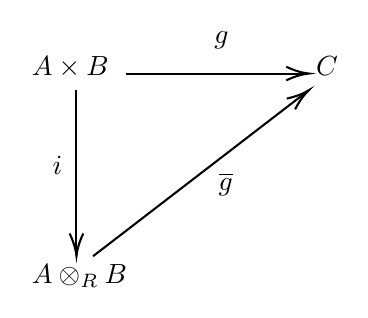
\begin{tikzpicture}[x=0.75pt,y=0.75pt,yscale=-1,xscale=1]
%uncomment if require: \path (0,476); %set diagram left start at 0, and has height of 476

%Straight Lines [id:da24913671305198637] 
\draw    (240,160) -- (240,238) ;
\draw [shift={(240,240)}, rotate = 270] [color={rgb, 255:red, 0; green, 0; blue, 0 }  ][line width=0.75]    (10.93,-3.29) .. controls (6.95,-1.4) and (3.31,-0.3) .. (0,0) .. controls (3.31,0.3) and (6.95,1.4) .. (10.93,3.29)   ;
%Straight Lines [id:da3370415482847726] 
\draw    (264,152) -- (350,152) ;
\draw [shift={(352,152)}, rotate = 180] [color={rgb, 255:red, 0; green, 0; blue, 0 }  ][line width=0.75]    (10.93,-3.29) .. controls (6.95,-1.4) and (3.31,-0.3) .. (0,0) .. controls (3.31,0.3) and (6.95,1.4) .. (10.93,3.29)   ;
%Straight Lines [id:da6219354900497076] 
\draw    (248,240) -- (350.41,161.22) ;
\draw [shift={(352,160)}, rotate = 142.43] [color={rgb, 255:red, 0; green, 0; blue, 0 }  ][line width=0.75]    (10.93,-3.29) .. controls (6.95,-1.4) and (3.31,-0.3) .. (0,0) .. controls (3.31,0.3) and (6.95,1.4) .. (10.93,3.29)   ;

% Text Node
\draw (217,142.4) node [anchor=north west][inner sep=0.75pt]    {$A\times B$};
% Text Node
\draw (217,242.4) node [anchor=north west][inner sep=0.75pt]    {$A\otimes _{R} B$};
% Text Node
\draw (354,142.4) node [anchor=north west][inner sep=0.75pt]    {$C$};
% Text Node
\draw (227,190.4) node [anchor=north west][inner sep=0.75pt]    {$i$};
% Text Node
\draw (305,130.4) node [anchor=north west][inner sep=0.75pt]    {$g$};
% Text Node
\draw (307,198.4) node [anchor=north west][inner sep=0.75pt]    {$\overline{g}$};


\end{tikzpicture}
\end{center}
\begin{proof}
We first prove the existence. Suppose $F$ is a free abelian group over $A\times B$. Then $g$ induces a homomorphism $g_1:F\to C$ that assign $(a,b)$ to $g(a,b)$. Since $g$ is a middle linear map, we have 
$$
\left( a_1+a_2,b \right) -\left( a_1,b \right) -\left( a_2,b \right) \mapsto g\left( a_1,b \right) +g\left( a_2,b \right) -g\left( a_1,b \right) -g\left( a_2,b \right) =0,
$$
and similarly assign the other generators of $K$ into zero. Therefore $K\subset\mathrm{Ker}g_1$. Therefore $g_1$ induces a map $\overline{g}:F/K\to C$ defined as $(a,b)+K\mapsto g(a,b)$. Since $F/K\cong A\otimes_RB$, we have 
$$
\overline{g}i\left( a,b \right) =\overline{g}\left( a\otimes b \right) =g\left( a,b \right) 
$$
for all $(a,b)\in F$, hence $\overline{g}i=g$. Note that $F$ is arbitrarily chosen, we have $\overline{g}i=g$ for all $(a,b)\in A\times B$.\par
Now suppose $h$ is another map that satisfy the condition. Then 
$$
h\left( a\otimes b \right) =hi\left( a,b \right) =g\left( a,b \right) =\overline{g}i\left( a,b \right) =\overline{g}\left( a\otimes b \right) ,
$$
whence $h=\overline{g}$ and the uniqueness is proved. By Theorem 2.55 we know that $A\otimes_RB$ is determined up to isomorphism by this property.
\end{proof}
\begin{corollary}
If $A_R$, $A_R^\prime$, $_RB$ and $_RB^\prime$ are modules over a ring $R$ and $f:A\to A^\prime$, $g:B\to B^\prime$ are $R$-module homomorphisms, then there is a unique group homomorphism $A\otimes_RB\to A^\prime\otimes_RB^\prime$ such that $a\otimes b\mapsto f(a)\otimes f(b)$ for all $a\in A$ and $b\in B$.
\end{corollary}
\begin{proof}
We first show that the assignment $(a,b)\mapsto f(a)\otimes g(b)$ defines a middle linear map $h:A\times B\to A^\prime\otimes_RB^\prime$. Note that 
$$
\begin{aligned}
h\left( a_1+a_2,b \right) &=f\left( a_1+a_2 \right) \otimes g\left( b \right) =\left( f\left( a_1 \right) +f\left( a_2 \right) \right) \otimes g\left( b \right) 
\\
&=f\left( a_1 \right) \otimes g\left( b \right) +f\left( a_2 \right) \otimes g\left( b \right) =h\left( a_1,b \right) +h\left( a_2,b \right) ,
\end{aligned}
$$
and the other rules may be proved analogously. By Theorem 5.49 we obtain the uniqueness of such $h$, and the proof is finished.
\end{proof}
\begin{note}\em
The uniqueness of Corollary 5.50 is denoted as follows: 
$$
f\otimes g:A\otimes _RB\rightarrow A^{\prime}\otimes _RB^{\prime}.
$$
If $f^\prime:A^\prime\to A^{\prime\prime}$ and $g:B^\prime\to B^{\prime\prime}$ are also $R$-module homomorphisms, then it is easy to verify that 
$$
\left( f^{\prime}\otimes g^{\prime} \right) \left( f\otimes g \right) =f^{\prime}f\otimes g^{\prime}g:A\otimes _RB\rightarrow A^{\prime\prime}\otimes _RB^{\prime\prime}.
$$
It follows readily that if $f$ and $g$ are isomorphisms, then $f\otimes g$ is a group isomorphism with inverse $f^{-1}\otimes g^{-1}$.
\end{note}
\begin{proposition}
If $A\overset{f}{\longrightarrow}B\overset{g}{\longrightarrow}C\longrightarrow 0$ is an exact sequence of left modules over a ring $R$ and $D$ is a right $R$-module, then 
$$
D\otimes _RA\overset{1_D\otimes f}{\longrightarrow}D\otimes _RB\overset{1_D\otimes g}{\longrightarrow}D\otimes _RC\longrightarrow 0
$$
is an exact sequence of abelian groups. An analogous statement holds for an exact sequence in the first variable.
\end{proposition}
\begin{proof}
We first prove that $1_D\otimes g$ is an epimorphism. Let $d\otimes c\in D\otimes_RC$, then since $g$ is an epimorphism, there exists some $b\in B$ such that $g(b)=c$, whence $(1_D\otimes g)(d\otimes b)=d\otimes c$, and hence $1_D\otimes g$ is an epimorphism.\par
Now we show that $\mathrm{Im}(1_D\otimes f)\cong\mathrm{Ker}(1_D\otimes g)$. We first show that $\mathrm{Im}(1_D\otimes f)\subset\mathrm{Ker}(1_D\otimes g)$. Since $gf=0$, we have 
$$
\left( 1_D\otimes g \right) \left( 1_D\otimes f \right) =1_D\otimes gf=1_D\otimes 0=0,
$$
whence $(1_D\otimes g)(1_D\otimes f)=0$, hence $\mathrm{Im}(1_D\otimes f)\subset\mathrm{Ker}(1_D\otimes g)$. Now we shall define the canonical epimorphism $\pi:D\otimes_RB\to(D\otimes_RB)/\mathrm{Im}(1_D\otimes f)$. Then there exists a homomorphism $\alpha:(D\otimes_RB)/\mathrm{Im}(1_D\otimes f)\to D\otimes_RC$ such that 
$$
\alpha \left( \pi \left( d\otimes b \right) \right) =\left( 1_D\otimes g \right) \left( d\otimes b \right) =d\otimes g\left( b \right) .
$$
We shall show that $\alpha$ is an isomorphism.\par
We show first that the map $\beta:D\times C\to(D\otimes_RB)/\mathrm{Im}(1_D\otimes f)$ given by $(d,c)\mapsto\pi(d\otimes b)$, where $g(b)=c$. We shall first show that $\pi$ is well-defined. It suffices to show that $g(b)=c$ is independent of the choice of $b$. Note that if $g(b)=g(b^\prime)$, then $b-b^\prime\in\mathrm{Ker}g=\mathrm{Im}f$, hence $f(a)=b-b^\prime$. Therefore 
$$
\pi \left( d\otimes b \right) =\pi \left( d\otimes \left( b^{\prime}+f\left( a \right) \right) \right) =\pi \left( d\otimes b^{\prime}+d\otimes f\left( a \right) \right) =\pi \left( d\otimes b^{\prime} \right) +\pi \left( d\otimes f\left( a \right) \right) =\pi \left( d\otimes b^{\prime} \right) ,
$$
which proved that $\pi$ is well-defined. It is routine to show that $\beta$ is middle linear. Then by the universal property we have $\overline{\beta}:D\otimes_RC\to(D\otimes_RB)/\mathrm{Im}(1_D\otimes f)$ such that 
$$
\overline{\beta }\left( d\otimes c \right) =\overline{\beta }i\left( d,c \right) =\beta \left( d,c \right) =\pi \left( d\otimes b \right) ,
$$
where $g(b)=c$. Therefore 
$$
\alpha \overline{\beta }\left( d\otimes c \right) =\alpha \left( \pi \left( d\otimes b \right) \right) =d\otimes g\left( b \right) =d\otimes c
$$
for all $d\times b\in D\otimes_RB$, therefore $\alpha \overline{\beta }=1_{D\otimes _RC}$. Similarly we have $\overline{\beta }\alpha =1_{\left( D\otimes _RB \right) /\mathrm{Im}\left( 1_D\otimes f \right)}$ and hence $\alpha$ is an isomorphism. Therefore $\mathrm{Im}\left( 1_D\otimes f \right) \cong \mathrm{Ker}\left( 1_D\otimes g \right) $, which finished the proof.
\end{proof}
\begin{note}\em
If $h:A_R\to _RA^\prime$ and $k:B_R\to _RB$ are module epimorphisms, then by the proof of Proposition 5.51 we know that $h\otimes k$ is an epimorphism. However this is not true if $h$ and $k$ are monomorphisms.
\end{note}
\begin{theorem}
Let $R$ and $S$ be rings and $_SA_R$, $_RB$, $C_R$ and $_RD_S$ (bi)modules as indicated.\par
(i) $A\otimes_RB$ is a left $S$ module such that $s(a\otimes b)=sa\otimes b$ for all $s\in S$, $a\in A$ and $b\in B$.\par
(ii) If $f:A\to A^\prime$ is a homomorphism of $S-R$ bimodules and $g:B\to B^\prime$ is an $R$-module homomorphism, then the induced map $f\otimes g:A\otimes_RB\to A^\prime\otimes_RB^\prime$ is a homomorphism of left $S$-modules.\par
(iii) $C\otimes_RD$ is a right $S$-module such that $(c\otimes d)s=c\otimes ds$ for all $c\in C$, $d\in D$ and $s\in S$.\par
(iv) If $h:C\to C^\prime$ is an $R$-module homomorphism and $k:D\to D^\prime$ a homomorphism of $R-S$ bimodules, then the induced map $h\otimes k:C\otimes_RD\to C^\prime\otimes_RD^\prime$ is a homomorphism of right $S$-modules.
\end{theorem}
\begin{proof}
We shall only prove (i) and (ii), the rest statements may be proved analogously. We first show that the operation is well-defined. For each $s\in S$ the map $A\times B\to A\otimes_RB$ given by $(a,b)\mapsto sa\otimes b$ is $R$-middle linear, and therefore induces a unique group homomorphism $\alpha_s:A\otimes_RB\to A\otimes_RB$ such that $\alpha_s(a\otimes b)=sa\otimes b$. For each element $u=\sum a_i\otimes b_i\in A\otimes_RB$ define $su$ to be the element 
$$
\alpha _s\left( u \right) =\alpha _s\left( \sum{a_i\otimes b_i} \right) =\sum{\alpha _s\left( a_i\otimes b_i \right)}=\sum{\left( sa_i\otimes b_i \right)}.
$$
Since $\alpha_s$ is a homomorphism, this action of $S$ is well-defined. It is now easy to verify that $A\otimes_RB$ is a left $S$-module.\par
Now for the second statement, take 
$$
\begin{aligned}
\left( f\otimes g \right) \left( a_1\otimes b_1+a_2\otimes b_2 \right) &=\left( f\otimes g \right) \left( \left( a_1+a_2 \right) \otimes \left( b_1+b_2 \right) \right) =f\left( a_1+a_2 \right) \otimes g\left( b_1+b_2 \right) 
\\
&=\left( f\left( a_1 \right) +f\left( a_2 \right) \right) \otimes \left( g\left( b_1 \right) +g\left( b_2 \right) \right) 
\\
&=f\left( a_1 \right) \otimes g\left( b_1 \right) +f\left( a_2 \right) \otimes g\left( b_2 \right) 
\\
&=\left( f\otimes g \right) \left( a_1\otimes b_1 \right) +\left( f\otimes g \right) \left( a_2\otimes b_2 \right) ,
\end{aligned}
$$
and the other rules may be verified analogously.
\end{proof}
\begin{note}\em
An important special case of Theorem 5.52 occurs when $R$ is a commutative ring and hence every $R$-module $A$ is an $R-R$ bimodule with $ra=ar$. In this case $A\otimes_RB$ is an $R-R$ bimodule with 
$$
r\left( a\otimes b \right) =ra\otimes b=ar\otimes b=a\otimes rb=a\otimes br=\left( a\otimes b \right) r
$$
for all $r\in R$, $a\in A$ and $b\in B
$.
\end{note}
If $R$ is a commutative ring, then the tensor product of $R$-modules may be characterized by a useful variation of Theorem 5.49. Let $A,B$ and $C$ be modules over a commutative ring $R$. A \textbf{bilinear map} from $A\times B$ to $C$ is a function $f:A\times B\to C$ such that for all $a,a_i\in A$, $b,b_i\in B$ and $r\in R$: 
$$
f\left( a_1+a_2,b \right) =f\left( a_1,b \right) +f\left( a_2,b \right) ;
$$
$$
f\left( a,b_1+b_2 \right) =f\left( a,b_1 \right) +f\left( a,b_2 \right) ;
$$
$$
f\left( ar,b \right) =f\left( a,rb \right) =rf\left( a,b \right) .
$$
Clearly every bilinear map is a middle linear map.
\begin{example}\em
If $A$ is a module over a commutative ring $R$ and $A^*$ is the dual of $A$, then the map $f:A\times A^*\to R$ given by $(a,f)\mapsto f(a)=\left<a,f\right>$ is a bilinear map.
\end{example}
\begin{example}\em
If $A$ and $B$ are modules over a commutative ring, then $A\otimes_RB$ is also a module over a commutative ring, and the canonical middle linear map $i:A\times B\to A\otimes_RB$ is also a bilinear map, which is called the \textbf{canonical bilinear map}.
\end{example}
\begin{theorem}
If $A,B$ and $C$ are modules over a commutative ring $R$ and $g:A\times B\to C$ is a bilinear map, then there is a unique $R$-module homomorphism $\overline{g}:A\otimes_RB\to C$ such that $\overline{g}i=g$, where $i:A\times B\to A\otimes_RB$ is the bilinear map. The module $A\otimes_RB$ is unique determined up to isomorphism by this property.
\end{theorem}
\begin{proof}
By the universal property of $A\otimes_RB$, it suffices to verify that $\overline{g}$ that defined in Theorem 5.49 is an $R$-module homomorphism. Let $r\in R$, then 
$$
\overline{g}\left( ra\otimes b \right) =g\left( ra,b \right) =rg\left( a,b \right) =r\overline{g}\left( a\otimes b \right) ,
$$
whence $\overline{g}$ is an $R$-module homomorphism. By Theorem 5.49 and Theorem 2.55 we know that $A\otimes_RB$ is determined up to isomorphism by this property.
\end{proof}
Theorem 5.53 provided another definition of $A\otimes_RB$ when $R$ is a commutative ring, that is, let $F$ be a free $R$-module over $A\times B$ and $K$ the submodule generated by elements 
$$
\left( a+a^{\prime},b \right) -\left( a,b \right) -\left( a^{\prime},b \right) ;
$$
$$
\left( a,b+b^{\prime} \right) -\left( a,b \right) -\left( a,b^{\prime} \right) ;
$$
$$
\left( ra,b \right) -r\left( a,b \right) ;
$$
$$
\left( a,rb \right) -\left( a,b \right) ;
$$
where $a,a^\prime\in A$ and $b,b^\prime\in B$, $r\in R$. Then $A\otimes_RB\cong F/K$.\par
We now return to modules over arbitrary rings.
\begin{theorem}
If $R$ is a ring with identity and $A_R$, $_RB$ are unitary $R$-modules, then there are $R$-module isomorphisms $A\otimes_RR\cong A$ and $R\otimes_RB\cong B$.
\end{theorem}
\begin{proof}
Since $R$ is an $R-R$ bimodule, $R\otimes_RB$ is a left $R$-module by Theorem 5.52. The assignment $(r,b)\mapsto rb$ defines a middle linear map $R\times B\to B$. By Theorem 5.49 it induces a homomorphism $\alpha:R\otimes_RB\to B$ given by $r\otimes b\mapsto rb$. We now show that $\alpha$ is an $R$-module homomorphism. Observe that 
$$
\alpha \left( sr\otimes b \right) =srb=s\left( rb \right) =s\alpha \left( r\otimes b \right) ,
$$
this proved that $\alpha$ is indeed a homomorphism of modules. Define $\beta:B\to R\otimes_RB$ given by $b\mapsto 1_R\otimes b$, then it is easy to verify that $\beta$ is also an $R$-module homomorphism and $\alpha\beta=1_R$, $\beta\alpha=1_{R\otimes_RB}$, therefore $\alpha$ and $\beta$ are $R$-module isomorphisms, and hence $R\otimes_RB\cong B$. Another assertion may be proved analogously.
\end{proof}
If $R$ and $S$ are rings and $A_R$, $_RB_S$, $_SC$ are (bi)modules, then both $(A\otimes_RB)\otimes_SC$ and $A\otimes_R(B\otimes_SC)$ are well-defined abelian groups.
\begin{theorem}
If $R$ and $S$ are rings and $A_R$, $_RB_S$, $_SC$ are (bi)modules, then there is an isomorphism 
$$
\left( A\otimes _RB \right) \otimes _SC\cong A\otimes _R\left( B\otimes _SC \right) .
$$
\end{theorem}
\begin{proof}
By definition, every element $v$ of $A\otimes_R(B\otimes_SC)$ is of the form 
$$
v=\sum_i{\left( u_i\otimes c_i \right)}=\sum_i{\left( \sum_j{\left( a_{ij}\otimes b_{ij} \right)}\otimes c_i \right)}=\sum_i{\sum_j{\left( a_{ij}\otimes b_{ij} \right) \otimes c_i}}.
$$
Therefore $A\otimes_R(B\otimes_SC)$ is generated by elements $a\otimes(b\otimes c)$. Similarly elements of $(A\otimes_RB)\otimes_SC$ is generated by elements $(a\otimes b)\otimes c$. Now we define 
$$
\alpha :\left( A\otimes _RB \right) \otimes _SC\rightarrow A\otimes _R\left( B\otimes _SC \right) 
$$
induced by the $S$-middle linear map 
$$
\left( A\otimes _RB \right) \times C\rightarrow A\otimes _R\left( B\otimes _SC \right) ,\hspace{0.5cm}\left( \sum_{i=1}^n{a_i\otimes b_i},c \right) \mapsto \sum_{i=1}^n{a_i\otimes \left( b_i\otimes c \right)}.
$$
Similarly there is an $R$-middle linear map that induces a homomorphism 
$$
\beta :A\otimes _R\left( B\otimes _SC \right) \rightarrow \left( A\otimes _RB \right) \otimes _SC.
$$
Verify that $\alpha\beta$ and $\beta\alpha$ are both identity maps, therefore $\alpha$ and $\beta$ are isomorphisms, and hence 
$$
\left( A\otimes _RB \right) \otimes _SC\cong A\otimes _R\left( B\otimes _SC \right) .
$$
This finished the proof.
\end{proof}
In the future we shall identify $\left( A\otimes _RB \right) \otimes _SC$ and $A\otimes _R\left( B\otimes _SC \right) $ under the isomorphism in Theorem 5.55 and simply write $A\otimes_RB\otimes_SC$. We further define recursively the $n$-fold tensor product: 
$$
A^1\otimes _{R_1}A^2\otimes _{R_2}\cdots \otimes _{R_n}A^{n+1},
$$
where $R_1,\cdots,R_n$ are rings and $A_{R_1}^1,_{R_1}A_{R_2}^2,\cdots,_{R_n}A^{n+1}$ are (bi)modules.
\begin{theorem}
Let $R$ be a ring, $A$ and $\{A_i:i\in I\}$ are right $R$-modules, $B$ and $\{B_j:j\in J\}$ left $J$-modules. Then there are group isomorphisms 
$$
\left( \bigoplus_{i\in I}{A_i} \right) \otimes _RB\cong \bigoplus_{i\in I}{\left( A_i\otimes _RB \right)};\hspace{0.5cm}A\otimes _R\left( \bigoplus_{j\in J}{B_j} \right) \cong \bigoplus_{j\in J}{\left( A\otimes _RB \right)}.
$$
\end{theorem}
\begin{proof}
Let $\iota_k$ and $\pi_k$ be the canonical injections and projections of $\bigoplus_{i\in I}A_i$. Therefore the family of homomorphisms $\iota_k\otimes 1_B:A_k\otimes_RB\to\left(\bigoplus_{i\in I}A_i\right)\otimes_RB$ induce a homomorphism 
$$
\alpha :\bigoplus_{i\in I}{\left( A_i\otimes _RB \right)}\rightarrow \left( \bigoplus_{i\in I}{A_i} \right) \otimes _RB,\hspace{0.5cm}\left\{ a_i\otimes b \right\} _{i\in I}\mapsto \left( \sum_{i\in I_0}{\iota _i\left( a_i \right)} \right) \otimes b,
$$
where $I_0$ is the set of all $i\in I$ such that $a_i\otimes b\ne 0$. Similarly the assignment $(u,b)\mapsto\{\pi_i(u)\otimes b\}_{i\in I}$ defines a middle linear map $\left(\bigoplus_{i\in I}A_i\right)\to\bigoplus_{i\in I}(A_i\otimes_RB)$ and induces a homomorphism 
$$
\beta :\left( \bigoplus_{i\in I}{A_i} \right) \otimes _RB\rightarrow \bigoplus_{i\in I}{\left( A_i\otimes _RB \right)},\hspace{0.5cm}u\otimes b\mapsto \left\{ \pi _i\left( u \right) \otimes b \right\} _{i\in I}.
$$
It is routine to verify that $\alpha\beta$ and $\beta\alpha$ are identity maps and hence $\alpha$ and $\beta$ are isomorphisms. This finished the proof.
\end{proof}
\begin{theorem}{(Adjoint Associativity)}
Let $R$ and $S$ be rings and $A_R$, $_RB_S$, $C_S$ (bi)modules, then there is an isomorphism of abelian groups 
$$
\alpha :\mathrm{Hom}_S\left( A\otimes _RB,C \right) \cong \mathrm{Hom}_R\left( A,\mathrm{Hom}_S\left( B,C \right) \right) .
$$
\end{theorem}
\begin{proof}
For each $f\in\mathrm{Hom}_S(A\otimes_RB,C)$ we define $\alpha:f\mapsto\alpha f$ such that $[(\alpha f)(a)](b)=f(a\otimes b)$. Then it is straight-forward verification of definitions that $\alpha$ is indeed an isomorphism.
\end{proof}
\begin{note}\em
Note that $\mathrm{Hom}_R(\cdot,\cdot)$ and $\mathrm{Hom}_S(\cdot,\cdot)$ consist of homomorphisms of right modules. Recall that the $R$-module structure of $\mathrm{Hom}_S(B,C)$ is given by $(gr)(b)=g(rb)$, where $r\in R$, $b\in B$ and $g\in\mathrm{Hom}_S(B,C)$.
\end{note}
We close this section with an investigation of the tensor product of free modules.
\begin{theorem}
Let $R$ be a ring with identity. If $A$ is a unitary right $R$-module and $F$ is a free left $R$-module with basis $Y$, then every element $u$ of $A\otimes_RF$ may be written uniquely in the form $u=\sum_{i=1}^na_i\otimes y_i$, where $a_i\in A$ and $y_i\in Y$ are distinct.
\end{theorem}
\begin{proof}
For each $y\in Y$, let $A_y$ be a copy of $A$ and consider the direct sum $\bigoplus_{y\in Y}A_y$. We first construct an isomorphism 
$$
\theta :A\otimes _RF\cong \bigoplus_{y\in Y}{A_y}
$$
as follows. Since $Y$ is a basis, $\{y\}$ is linearly independent for each $y\in Y$. Therefore there the $R$-module epimorphism $\varphi:R\to Ry$ given by $r\mapsto ry$ is actually an isomorphism. Therefore by Theorem 5.54 there is an isomorphism for each $y$ that 
$$
A\otimes _RRy\overset{1_A\otimes _R\varphi ^{-1}}{\longrightarrow}A\otimes _RR\cong A=A_y.
$$
Thus there is an isomorphism $\theta$ defined as follows: 
$$
A\otimes _RF\cong A\otimes _R\left( \bigoplus_{y\in Y}{Ry} \right) \cong \bigoplus_{y\in Y}{\left( A\otimes _RRy \right)}\cong \bigoplus_{y\in Y}{A_y}.
$$
For every $a\in A$ and $z\in Y$, we have $\theta(a\otimes z)=\{u_y\}\in\bigoplus_{y\in Y}A_y$, where $u_z=a$ and $u_y=0$ for $y\ne z$. Now for each nonzero $v\in\bigoplus_{y\in Y}A_y$ we have 
$$
v=\sum_{i=1}^n{\iota _{y_i}\left( a_i \right)}=\sum_{i=1}^n{\theta \left( a_i\otimes y_i \right)}.
$$
Therefore 
$$
u=\theta ^{-1}\left( v \right) =\theta ^{-1}\left( \sum_{i=1}^n{\theta \left( a_i\otimes y_i \right)} \right) =\sum_{i=1}^n{a_i\otimes y_i},
$$
which finished the proof.
\end{proof}
It follows directly from Theorem 5.58 that, if $R$ is a ring with identity and $A_R$, $_RB$ free $R$-modules with basis $X$ and $Y$, then $A\otimes_RB$ is a free module over $R$ with basis $W=\{x\otimes y:x\in X,y\in Y\}$. Therefore $|A\otimes_RB|=|X||Y|$.
\begin{center}
\begin{large}
    \textbf{Exercises for 5.5}
\end{large}
\end{center}
Note that $R$ is a ring and $\otimes=\otimes_\mathbb{Z}$.
\begin{problem}\em
If $R=\mathbb{Z}$, then the condition (iii) in Definition 5.48 is superfluous.
\end{problem}
\begin{proof}
It suffices to notice that 
$$
f\left( ar,b \right) =f\left( \underset{r\,\,\mathrm{times}}{\underbrace{a+a+\cdots +a}},b \right) =rf\left( a,b \right) =f\left( a,\underset{r\,\,\mathrm{times}}{\underbrace{b+b+\cdots +b}} \right) =f\left( a,rb \right) .
$$
Therefore (i) and (ii) together implies (iii) when $R=\mathbb{Z}$.
\end{proof}
\begin{problem}\em
Let $A$ and $B$ be abelian groups.\par
(a) For each $m\in\mathbb{N}$, $A\otimes\mathbb{Z}_m\cong A/mA$.\par
(b) $\mathbb{Z}_m\otimes\mathbb{Z}_n\cong\mathbb{Z}_{(m,n)}$, where $(m,n)$ denote the greatest common divisor of $m$ and $n$.\par
(c) Describe $A\otimes B$, when $A$ and $B$ are finitely generated.
\end{problem}
\begin{proof}
(a) By Theorem 5.54 we know that $A\cong A\otimes\mathbb{Z}$. Consider the canonical projection $\pi:A\otimes\mathbb{Z}_m\to A\otimes\mathbb{Z}$, then $\mathrm{Ker}\pi=A\otimes m\mathbb{Z}=m(A\otimes\mathbb{Z})\cong mA$. Therefore 
$$
A\otimes \mathbb{Z} _m\cong \left( A\otimes \mathbb{Z} \right) /\mathrm{Ker}\pi \cong \left( A\otimes \mathbb{Z} \right) /m\left( A\otimes \mathbb{Z} \right) \cong A/mA,
$$
whence $A\otimes\mathbb{Z}_m\cong A/mA$.\par
(b) By (a) we have 
$$
\mathbb{Z} _m\otimes \mathbb{Z} _n\cong \mathbb{Z} _m/n\mathbb{Z} _m\cong \mathbb{Z} _{\left( m,n \right)},
$$
which finished the proof.\par
(c) Since $A$ and $B$ are finitely generated, we may assume that $A\cong\bigoplus_{i\in I}\mathbb{Z}/p_i^{\alpha_i}\mathbb{Z}$, and $B\cong\bigoplus_{j\in J}\mathbb{Z}/q_j^{\beta_j}\mathbb{Z}$, where $p_i$ and $q_j$ are prime numbers and $\alpha_i$, $\beta_j\in\mathbb{N}$. Therefore 
$$
\begin{aligned}
A\otimes B&\cong \left( \bigoplus_{i\in I}{\mathbb{Z} /p_{i}^{\alpha _i}\mathbb{Z}} \right) \otimes \left( \bigoplus_{j\in J}{\mathbb{Z} /q_{j}^{\beta _j}\mathbb{Z}} \right) 
\\
&\cong \bigoplus_{i\in I}{\bigoplus_{j\in J}{\left( \mathbb{Z} /p_{i}^{\alpha _i}\mathbb{Z} \right) \otimes \left( \mathbb{Z} /q_{j}^{\beta _j}\mathbb{Z} \right)}}\cong \bigoplus_{i\in I}{\bigoplus_{j\in J}{\mathbb{Z} /\left( p_{i}^{\alpha _i},q_{j}^{\beta _j} \right) \mathbb{Z}}}.
\end{aligned}
$$
Since $p_i$ and $q_j$ are primes, we conclude that 
$$
A\otimes B\cong \bigoplus_{k\in K}{\mathbb{Z} _k},\hspace{0.5cm}K=\left\{ p^{\alpha}:\text{$p^\alpha$ is the common prime elementary divisors of $A$ and $B$}\right\} .
$$
Therefore $A\otimes B\cong\bigoplus_{k\in K}\mathbb{Z}_k$ with given $K$ as above.
\end{proof}
\begin{problem}\em
If $A$ is a torsion abelian group and $\mathbb{Q}$ the additive group of rationals, then \par
(a) $A\otimes\mathbb{Q}=0$;\par
(b) $\mathbb{Q}\otimes\mathbb{Q}\cong\mathbb{Q}$.
\end{problem}
\begin{proof}
(a) Take $a\otimes r$. Since $a\in A$ is torsion, there exists some $m\in\mathbb{Z}$ such that $ma=0$. Therefore 
$$
a\otimes r=a\otimes m\cdot \frac{r}{m}=m\left( a\otimes \frac{r}{m} \right) =ma\otimes \frac{r}{m}=0\otimes \frac{r}{m}=0.
$$
Therefore every generator of $A\otimes\mathbb{Q}$ is zero, hence $A\otimes\mathbb{Q}=0$.\par
(b) Let $r\otimes s\in\mathbb{Q}\otimes\mathbb{Q}$ with $r,s\in\mathbb{Q}$. Then 
$$
r\otimes s=\frac{a}{b}\otimes \frac{c}{d}=1\otimes \left( \frac{a}{b} \right) \cdot \left( \frac{c}{d} \right) =1\otimes r^{\prime},
$$
hence every generator of $\mathbb{Q}\otimes\mathbb{Q}$ is of the form $1\otimes r$. Now we define $1\otimes r\mapsto r$, it is easy to see an isomorphism and hence $\mathbb{Q}\otimes\mathbb{Q}\cong\mathbb{Q}$.
\end{proof}
\begin{problem}\em
Let $u\in A\otimes_RB$, give examples to show that their may be $u\ne a\otimes b$ for all $a\in A$ and $b\in B$.
\end{problem}
\begin{proof}
We consider $\mathbb{R}^2\otimes_{\mathbb{R}^2}\mathbb{R}^2$ and $(e_1,e_2)$ the standard basis for $\mathbb{R}^2$. We show that $e_1\otimes e_2+e_2\otimes e_1$ can't be expressed in the form $a\otimes b$. Suppose not, then let $a=a_1e_1+a_2e_2$, and $b=b_1e_1+b_2e_2$. Therefore 
$$
\begin{aligned}
a\otimes b&=\left( a_1e_1+a_2e_2 \right) \otimes \left( b_1e_1+b_2e_2 \right) 
\\
&=a_1b_1\left( e_1\otimes e_1 \right) +a_1b_2\left( e_1\otimes e_2 \right) +a_2b_1\left( e_2\otimes e_1 \right) +a_2b_2\left( e_2\otimes e_2 \right) ,
\end{aligned}
$$
which implies 
$$
\begin{cases}
	a_1b_1=0,\\
	a_1b_2=1,\\
	a_2b_1=1,\\
	a_2b_2=0,\\
\end{cases}
$$
which is impossible! Therefore $e_1\otimes e_2+e_2\otimes e_1$ cannot be written into the form $a\otimes b$.
\end{proof}
\begin{problem}\em
If $A^\prime$ is a submodule of the right $R$-module $A$ and $B^\prime$ is a submodule of the left $R$-module $B$, then $A/A^\prime\otimes B/B^\prime\cong(A\otimes_RB)/C$, where $C$ is the subgroup of $A\otimes_RB$ generated by elements $a\otimes b^\prime$ and $a^\prime\otimes b$, where $a\in A$, $b\in B$, $a^\prime\in A^\prime$ and $b^\prime\in B^\prime$.
\end{problem}
\begin{proof}
Consider the map $(a+A^\prime,b+B^\prime)\mapsto(a\otimes b)+C$, which is a middle linear map from $A/A^\prime\times B/B^\prime$ to $A\otimes_RB/C$. Therefore it induced a map $\alpha:A/A^\prime\otimes_R B/B^\prime\to(A\otimes_RB)/C$ that assigns $(a+A^\prime)\otimes(b+B^\prime)$ to $(a\otimes b)+C$. Now we define $\beta:(A\otimes_RB)/C\to A/A^\prime\otimes B/B^\prime$ by $(a\otimes b)+C\to(a+A^\prime)\otimes(b+B^\prime)$, then it is easy to verify that $\beta$ is a homomorphism of abelian groups and $\alpha\beta=1_{(A\otimes_RB)/C}$, $\beta\alpha=1_{A/A^\prime\otimes_RB/B^\prime}$, therefore both $\alpha$ and $\beta$ are isomorphisms, and hence $A/A^\prime\otimes_RB/B^\prime\cong(A\otimes_RB)/C$.
\end{proof}
\begin{problem}\em
Let $f:A_R\to A_R^\prime$ and $g:_RB\to _RB^\prime$ be $R$-module homomorphisms. What is the difference between the homomorphism $f\otimes g$ as given in Remark 5.7 and the element $f\otimes g$ of the tensor product of abelian groups $\mathrm{Hom}_R(A,A^\prime)\otimes_R\mathrm{Hom}_R(B,B^\prime)$?
\end{problem}
\begin{proof}
The first $f\otimes g$ in Remark 5.7 is an element of $\mathrm{Hom}(A\otimes_RA^\prime,B\otimes_RB^\prime)$. Indeed, we may define an canonical injection 
$$\mathrm{Hom}_R(A\otimes_RA^\prime,B\otimes_RB^\prime)\to\mathrm{Hom}_R(A,A^\prime)\otimes_R\mathrm{Hom}_R(B,B^\prime),$$
and the injection is an isomorphism when all spaces here are finite-dimensional.
\end{proof}
\begin{problem}\em
Let $0\longrightarrow A\overset{f}{\longrightarrow}B\overset{g}{\longrightarrow}C\longrightarrow 0$ be a short exact sequence of left $R$-modules and $D$ a right $R$-module. Then $0\longrightarrow D\otimes _RA\overset{1\otimes f}{\longrightarrow}D\otimes _RB\overset{1\otimes g}{\longrightarrow}D\otimes _RC\longrightarrow 0$ is a short exact sequence of abelian groups under any one of the following hypothesis:\par
(a) $0\longrightarrow A\overset{f}{\longrightarrow}B\overset{g}{\longrightarrow}C\longrightarrow 0$ is split exact;\par
(b) $R$ has an identity and $D$ is a free right $R$-module;\par
(c) $R$ has an identity and $D$ is a projective unitary right $R$-module.
\end{problem}
\begin{proof}
This is an analogous statement of Theorem 5.38, and the proof here may be proceed in a similar way. We skip the details.
\end{proof}
\begin{problem}\em
(a) If $I$ is a right ideal of a ring $R$ with identity and $B$ a left $R$-module, then there is a group isomorphism $R/I\otimes_RB\cong B/IB$, where $IB$ is the subgroup of $B$ generated by elements of the form $ib$.\par
(b) Let $R$ be a commutative ring and $I$, $J$ are ideals of $R$. Then there is $R$-module isomorphism $R/I\otimes_RR/J\cong R/(I+J)$.
\end{problem}
\begin{proof}
(a) We consider the short exact sequence 
$$
0\longrightarrow I\overset{\iota}{\longrightarrow}R\overset{\pi}{\longrightarrow}R/I\longrightarrow 0,
$$
by Proposition 5.51 we know that the sequence 
$$
B\otimes _RI\overset{1_B\otimes \iota}{\longrightarrow}B\otimes _RR\overset{1_B\otimes \pi}{\longrightarrow}B\otimes _RR/I\longrightarrow 0
$$
is exact. Therefore 
$$
\mathrm{Ker}\left( 1_B\otimes \pi \right) =\mathrm{Im}\left( 1_B\otimes \iota \right) \cong IB
$$
and hence 
$$
B\otimes _RR/I\cong \left( B\otimes _RR \right) /\mathrm{Ker}\left( 1_B\otimes \pi \right) \cong B/IB,
$$
this finished the proof.\par
(b) We define $\alpha:(r+I)\otimes(s+J)\mapsto rs+(I+J)$, then $\alpha$ is easily verified a well-defined $R$-module homomorphism. Then consider $\beta:a+(I+J)\mapsto (a+I)\otimes(1+J)$, then $\beta$ is also a well-defined $R$-module homomorphism and $\alpha\beta=1_{R/(I+J)}$, $\beta\alpha=1_{R/I\otimes_RR/J}$, therefore $\alpha$ is an isomorphism and hence $R/I\otimes_RR/J\cong R/(I+J)$.
\end{proof}
\subsection{Modules over a Principal Ideal Domain}
The chief purpose of this section is to determine the structure of all finitely generated modules over a principal ideal domain. Virtually all of the structure theorems for finitely generated abelian groups carry over to such modules. We shall show that just as in the case of abelian groups every finitely generated module may be decomposed in two ways as a direct sum of cyclic submodules. Each decomposition provides a set of invariants for the given module (that is, two modules have the same 
invariants if and only if they are isomorphic). Thus each method of decomposition leads to a complete classification (up to isomorphism) of all finitely generated modules over a principal ideal domain. Here and throughout this section "module" means "unitary module".\par
We begin with free modules over a principal ideal domain $R$. Since $R$ has the invariant dimension property, the rank of a free $R$-module is well defined.
\begin{theorem}
Let $F$ be a free module over a principal ideal domain $R$ and $G$ a submodule of $F$. Then $G$ is a free $R$-module and $\mathrm{rank}G\le\mathrm{rank}F$.
\end{theorem}
\begin{proof}
Let $X=\{x_i:i\in I\}$ be a basis of $F$. Then $F\cong\bigoplus_{i\in I}Rx_i$, where each $Rx_i$ is isomorphic to $R$. Choose a well ordering $\prec$ of the set $I$, and let $J=I\cup\{\alpha\}$, where $\alpha\notin I$. Let $\alpha$ satisfy $i\prec\alpha$ for all $i\in I$. Such an operation guarantees that all elements in $I$ has an immediate successor in $J$. Now for each $j\in J$, we define $F_j$ be the submodule generated by $\{x_i:i\prec j\}$. We claim that $F_j$ has the following properties:\par
(i) $j\prec k$ if and only if $F_j\subset F_k$. Observe that $\{x_i:i\prec j\}$ is hence a subset of $\{x_i:i\prec k\}$, therefore $F_j\subset F_k$. The other direction follows from an analogous argument.\par
(ii) $\bigcup_{j\in J}F_j=F$. The direction $\bigcup_{j\in J}F_j\subset F$ since $F_j\subset F$ for each $j\in J$. To prove the converse inclusion, for each $x_k\in F$, since $J$ is well-ordered, there exists some $j\in J$ such that $k\prec j$, therefore $x_k\in F_j$ and hence $F\subset\bigcup_{j\in J}F_j$.\par
(iii) For each $i\in I$, $F_{i+1}/F_i\cong Rx_i\cong R$. We consider the canonical projection 
$$
\pi _{i+1}:F_{i+1}\cong \bigoplus_{k\prec i+1}{Rx_k}\rightarrow Rx_i,\sum{r_kx_k}\mapsto r_ix_i.
$$
By the first isomorphism theorem, we have $\mathrm{Ker}\pi=F_k$, therefore $Rx_i\cong F_{k+1}/\mathrm{Ker}\pi _{k+1}\cong F_{k+1}/F_k$.\par
For each $j\in J$, let $G_j=G\cap F_j$. We claim that $G_j$ has the following properties: \par
(iv) $j\prec k$ implies $G_j\subset G_k$. Note that $G_j=G\cap F_j\subset G\cap F_k=G_k$, therefore $G_j\subset G_k$.\par
(v) $\bigcup_{j\in J}G_j=G$. Note that 
$$
\bigcup_{j\in J}{G_j}=\bigcup_{j\in J}{\left( G\cap F_j \right)}=G\cap \left( \bigcup_{j\in J}{F_j} \right) =G,
$$
therefore $F_{i+1}/F_i\cong Rx_i\cong R$.\par
(vi) For each $i\in I$, $G_i=G_{i+1}\cap F_i$. Note that $G_{i+1}\cap F_i=\left( G\cap F_{i+1} \right) \cap F_i=G\cap \left( F_{i+1}\cap F_i \right) $, while $F_{i+1}\subset F_i$, we conclude that $G_i=G_{i+1}\cap F_i$.\par
Now $G_{i+1}/G_i\cong G_{i+1}/\left( G_{i+1}\cap F_i \right) \cong \left( G_{i+1}+F_i \right) /F_i$. Since $(F_i+G_{i+1})/F_i$ is a submodule of $F_{i+1}/F_i$, we have $G_{i+1}/G_i$ is isomorphic to a submodule of $R$. But every submodule of $R$ is an ideal of $R$ and $R$ is a principal ideal domain, therefore $G_{i+1}/G_i$ is of the form $(c)$, where $c\in R$. Therefore $G_{i+1}/G_i$ is a free submodule of $R$ with rank $0$ or $1$ depending on whether $c=0$. Hence $G_{i+1}/G_i$ is projective, and hence the exact sequence 
$$
0\longrightarrow G_i\overset{\subset}{\longrightarrow}G_{i+1}\overset{\pi}{\longrightarrow}G_{i+1}/G_i\longrightarrow 0
$$
is split exact, hence $G_{i+1}\cong G_i\oplus G_{i+1}/G_i\cong G_i\oplus Rb_i$, where $b_i\in G_{i+1}-G_i$ and $Rb_i\cong R$ if $b_i\ne 0$, $Rb_i=0$ if $b_i=0$(under which circumstance $G_{i+1}/G_i=0$). Thus $b_i\in G$ is defined for each $i\in I$. Let $B=\{b_i:i\in I\}$, then $|B|\le|I|=\mathrm{rank}F$. Now it suffices to show that $B$ is a basis of $G$.\par
To prove this, we first show that $B$ is linearly independent. Suppose $0=u=\sum_jr_jb_j$ a finite sum. Let $k$ be the largest index such that $r_k\ne 0$. Then 
$$
u=\sum_{j\prec k}{r_jb_j}+r_kb_k\in G_k\oplus Rb_k=G_{k+1}.
$$
However $u=0$, this implies $r_k=0$, a contradiction! Therefore $r_j=0$ for all $j\in J$. Therefore $B$ is linearly independent.\par
Finally we show that $B$ spans $G$. We prove by transfinite induction. Suppose that $B_j$ spans $G_j$ for all $j\prec k$ and let $u\in G_k$. Now we break the proof into two parts.\par
(i) Suppose $k=j+1$ for some $j\in I$. Then $G_k=G_{j+1}\cong G_j\oplus Rb_j$ and $u=v+rb_j$ with $v\in G_j$. By the induction hypothesis we know that $v$ is a finite sum $\sum r_ib_i$ with $r_i\in R$ and $b_i\in B_j\subset B_k$. Therefore $u=\sum r_ib_i+rb_k$, hence $B_k$ spans $G_k$.\par
(ii) There are no $j\in J$ such that $k=j+1$. Since $u\in G_k=G\cap F_k$, $u$ is a finite sum $u=\sum r_jx_j$ with $j\prec k$. If $t$ is the largest index such that $r_t\ne 0$, then $u\in F_{t+1}$ with $t+r\prec k$ by hypothesis. Therefore $u\in G\cap F_{t+1}$ with $t+1\prec k$. By the induction hypothesis $u$ is a linear combination of elements of $B_{t+1}$, which is a subset of $B_k$. Hence $B_k$ spans $G_k$.
\end{proof}
An immediate consequence of Theorem 5.59 is as follows: 
\begin{corollary}
Let $R$ be a principal ideal domain. If $A$ is a finitely generated $R$-module generated by $n$ elements, then every submodule of $A$ may be generated by $m$ elements with $m\le n$.
\end{corollary}
\begin{proof}
See Theorem 5.59, and replace $(I,\prec)$ with $(\mathbb{N},\le)$.
\end{proof}
\begin{corollary}
A unitary module $A$ over a principal ideal domain is free if and only if $A$ is projective.
\end{corollary}
\begin{proof}
If $A$ is free, then $A$ is projective. Conversely, there exists a free module $F$ and $f:F\to A$ such that $f$ is an epimorphism, and hence the exact sequence 
$$
0\longrightarrow \mathrm{Ker}f\overset{\subset}{\longrightarrow}F\overset{f}{\longrightarrow}A\longrightarrow 0
$$
is split exact, hence $F\cong A\oplus\mathrm{Ker}f$. Therefore $A$ is isomorphic to a submodule of $F$, and by Theorem 5.59 we have $A$ free.
\end{proof}
We now develop the analogous of the order of an element in a group and of the torsion subgroup of abelian group.
\begin{theorem}
Let $A$ be a left module over an integral domain $R$ and for each $a\in A$ let $\mathcal{O}_a=\{r\in R:ra=0\}$.\par
(i) $\mathcal{O}_a$ is an ideal of $R$ for each $a\in A$.\par
(ii) $A_t=\{a\in A:\mathcal{O}_a=0\}$ is a submodule of $A$.\par
(iii) For each $a\in A$ there is an isomorphism of left modules 
$$R/\mathcal{O}_a\cong Ra=\{ra:r\in R,a\in A\}.$$\par
Let $R$ be a principal ideal domain and $p\in R$ a prime.\par
(iv) If $p^ia=0$, then $\mathcal{O}_a=(p^j)$ with $0\le j\le i$.\par
(v) If $\mathcal{O}_a=(p^i)$, then $p^ja\ne 0$ for all $j$ such that $0\le j<i$.
\end{theorem}
\begin{proof}
Note that prime and irreducible coincide over a principal ideal domain.\par
(i) Let $r_a\in\mathcal{O}_a$. Then for each $r\in R$, we have $rr_aa=0$, whence $rr_a\in\mathcal{O}_a$. Therefore $\mathcal{O}_a$ is an ideal of $R$.\par
(ii) Let $a,b\in A_t$, then $\mathcal{O}_a\ne 0$ and $\mathcal{O}_b\ne 0$ implies $r_1a=0$, $r_2b=0$ for some $r_1,r_2\in R$. Let $r=r_1r_2$, then $r(a+b)=0$ and hence $\mathcal{O}_{a+b}\ne 0$, hence $a+b\in A_t$. Similarly one may show that $ra\in A_t$ for all $r\in R$. Hence $A_t$ is a submodule of $A$.\par
(iii) Consider the canonical projection $\pi:R\to Ra$ given by $r\mapsto ra$. Clearly $\mathrm{Ker}\pi=\mathcal{O}_a$, hence by the first isomorphism theorem we have $Ra\cong R/\mathrm{Ker}\pi=R/\mathcal{O}_a$.\par
(iv) Since $p^ia=0$, we have $(p^i)\subset\mathcal{O}_a$. Therefore $(p^i)\subset (a)$ and hence $a\mid p^i$. Therefore $\mathcal{O}_a=(p^j)$ with $0\le j\le i$.\par
(v) Suppose $p^ka=0$ with $k$ an integer. Then by (iv) we have $\mathcal{O}_a=(p^i)$ with $k\ge i$. Therefore if $p^ja\ne 0$, we must have $0\le j<i$.
\end{proof}
\begin{note}\em
Let $A$ be a module over an integral domain. Then the ideal $\mathcal{O}_a$ defined in Theorem 5.62 is called the \textbf{order ideal} of $a\in A$. The submodule $A_t$ is called the \textbf{torsion submodule} of $A$. If $A_t=A$, then $A$ is called the \textbf{torsion module}, and if $A_t=0$, then $A$ is called the \textbf{torsion-free module}.
\end{note}
Let $A$ be a module over a principal ideal domain $R$. The order ideal of $a\in A$ is a principal ideal, say $\mathcal{O}_a=(r)$. Then $a\in A$ is said to have \textbf{order $r$}. The element $r$ is unique up to multiplication to a unit. The cyclic submodule $Ra$ generated by $a$ is said to be \textbf{cyclic of order $r$}. An immediate consequence of the definition is that if an element $a\in A$ has order $r$, where $r$ is a unit, then $a=0$, since $a=1_Ra=r^{-1}ra=0$.\par
\begin{example}\em
If $R$ is a principal ideal domain and $r\in R$, then the quotient ring $R/(r)$ is a cyclic $R$-module with generator $a=1_R+(r)$. Clearly $\mathcal{O}_a=(r)$, whence $a$ has order $r$ and $R/(r)$ is cyclic of order $r$. Theorem 5.62(iii) shows that every cyclic module $C$ over a principal ideal domain $R$ is isomorphic to $R/(r)$, where $(r)=\mathcal{O}_a$ and $a$ is a generator of $C$.
\end{example}
\begin{example}\em
Let $R=\mathbb{Z}$ and $A$ be an additive abelian group. Suppose the group theoretic order of $a\in A$ is finite. Then $\mathcal{O}_a=(n)$, where $|n|$ is the order of $a$. If $a\in A$ has infinite order, then $\mathcal{O}_a=(0)$. In either case $\mathbb{Z}a$ is a cyclic subgroup $\left<a\right>$ generated by $a$. Furthermore, $\mathbb{Z}a\cong\mathbb{Z}/(n)\cong\mathbb{Z}_n$ with $n\ne 0$, and $\mathbb{Z}a\cong\mathbb{Z}/(0)\cong\mathbb{Z}$ if $\mathcal{O}_a=(0)$.
\end{example}
\begin{theorem}
A finitely generated torsion-free module $A$ over a principal ideal domain $R$ is free.
\end{theorem}
\begin{proof}
We may assume $A\ne 0$. Let $X$ be a set of generators of $A$. If $x\in X$, then there exists some $r\in R$ such that $rx=0$ since $A$ is torsion-free. Therefore we may take a largest subset $S=\{x_1,\cdots,x_k\}$ of $X$ such that elements of $S$ are linearly independent. Let $F$ be a submodule of $A$ generated by $S$, then $F$ is clearly free over $R$. Now suppose $y\in X-S$. Then by the maximality of $S$ there exists some $r_y\in R$ such that $r_yy+r_1x_1+\cdots+r_kx_k=0$ with $r_i\ne 0$ and $r_y\ne 0$. Therefore $r_yy=-\sum_{i=1}^kr_ix_i$. Let $r=\prod_{y\in X-S}r_y$, we have $rX\subset F$. Since $X$ generated $A$, we have $rA\subset F$ a subset of $F$, therefore $rA$ is free. Now observe that $A$ is torsion-free, we have $A\cong rA\subset F$, hence $A$ is free by Theorem 5.59.
\end{proof}
We now determine the structure of a finitely generated module over a principal ideal domain. We shall proceed in three steps. We show first that $A$ is a direct sum of a torsion module and a free module. Every torsion module is a direct sum of "$p$-primary modules", and finally every $p$-primary module is a direct sum of cyclic modules.
\begin{theorem}
If $A$ is a finitely generated module over a principal ideal domain $R$, then $A\cong A_t\oplus F$, where $F$ is a free module $A/A_t$.
\end{theorem}
\begin{proof}
Clearly $A/A_t$ is a torsion-free module, hence $A/A_t$ is a free module by theorem 5.63. Now by Corollary 5.61 we know that $A/A_t$ is a projective module over $R$, therefore the short exact sequence $0\longrightarrow A_t\overset{\subset}{\longrightarrow}A\overset{\pi}{\longrightarrow}A/A_t\longrightarrow 0$ is split exact, hence $A\cong A_t\oplus A/A_t$.
\end{proof}
\begin{theorem}
Let $A$ be a torsion module over a principal ideal domain $R$ and for each prime $p\in R$ let $A(p)=\{a\in A:\text{$a$ has order a power of $p$}\}$.\par
(i) $A(p)$ is a submodule of $A$ for each prime $p\in R$.\par
(ii) $A=\bigoplus A(p)$, where the sum is taken over all primes $p\in R$. If $A$ is finitely generated, then only finitely many of $A(p)$ is nonzero.
\end{theorem}
\begin{proof}
(i) Suppose $a,b\in A(p)$. Suppose $\mathcal{O}_a=(p^i)$ and $\mathcal{O}_b=(p^j)$, then let $k=\max\{i,j\}$, we have $p^k(a+b)=0$, and hence $\mathcal{O}_{a+b}=(p^r)$ with $0\le r\le k$, hence $a+b\in A(p)$. Similarly we have $ra\in A(p)$ with $a\in A(p)$ and $r\in R$, therefore $A(p)$ is a submodule of $A$.\par
(ii) Let $\mathcal{P}$ be the set of all prime elements in $A$. We first show that $\{A(p):p\in\mathcal{P}\}$ generated the whole $A$. Let $0\ne a\in A$ and $\mathcal{O}_a=(r)$. Suppose $r=p_{1}^{a_1}p_{2}^{a_2}\cdots p_{k}^{a_k}$ with $p_i\in\mathcal{P}$ distinct and $n_i\in\mathbb{N}$. Now define $r_j=p_{1}^{a_1}\cdots p_{j-1}^{a_{j-1}}p_{j+1}^{a_{j+1}}\cdots p_{k}^{a_k}$ with $j=1,2,\cdots,k$. Clearly $\{r_j\}_{j=1}^k$ are relatively prime and hence there exists some $s_1,\cdots,s_k\in R$ such that $s_1r_1+\cdots+s_kr_k=1_R$. Therefore 
$$
u=1_Ru=\left( s_1r_1+s_2r_2+\cdots +s_kr_k \right) u=s_1r_1u+s_2r_2u+\cdots +s_kr_ku.
$$
Now observe that $p_{j}^{a_j}s_jr_ju=s_jru=0$, we have $s_jr_ju\in A(p_j)$, hence we proved that $A(p)$ generated the whole $A$.\par
Now we show that the sum is direct sum. Suppose $a\in A(p)\cap A_1$, where $A_1$ is generated by $\{A(q):q\in\mathcal{P}-\{p\}\}$. Therefore there exists some $i\in\mathbb{N}$ such that $p^ia=0$ and $da=0$, where $d=\prod_{q\in\mathcal{P}-\{p\}}q^{m_q}$, where $m_q\in\mathbb{N}$. Clearly $d$ and $p$ are relatively prime, therefore there exists $r$ and $s\in R$ such that $rp+sd=1_R$, hence $a=rpa+sda=0$, therefore $A(p)\cap A_1=0$ and hence the sum is direct sum.
\end{proof}
In order to determine the structure of finitely generated modules in which every element has order a power of a prime $p$, we shall need a lemma:
\begin{lemma}\em
Let $A$ be a module over a principal ideal domain $R$ such that $p^nA=0$ and $p^{n-1}A\ne 0$ for some prime $p\in R$ and positive integer $n$. Let $a$ be an element of $A$ of order $p^n$. Then there is a submodule $C$ of $A$ such that $A\cong Ra\oplus C$.
\end{lemma}
\begin{proof}
We show that $Ra$ is an injective $R$-submodule of $A$. First observe that every $R$-module may be regarded as an $R/(p^n)$-module with a pullback along $R\to R/(p^n)$, we shall show that $Ra$ is an injective $R/(p^n)$ submodule of $A$. By Theorem 5.62 we know that $Ra\cong R/\mathcal{O}_a=R/(p^n)$, therefore we shall show that $R/(p^n)$ is an injective module over itself.\par
We prove by first determining the ideals of $R/(p^n)$. Clearly $(p^i+(p^n))$ are ideals of $R/(p^n)$ with $0\le i<n$. We now show that these are the only proper ideals of $R/(p^n)$. Since $R$ is a principal ideal domain, it suffices to consider ideals of the form $(q^j)$, where $q$ is another prime element in $R$ distinct from $p$. Then clearly $p^n$ and $q$ are relatively prime, hence there exists $r$ and $s\in R$ such that $rp^n+sq=1_R$, therefore $q$ is invertible in $R/(p^n)$ and hence the only nonunits in $R/(p^n)$ are $p^i$ with $1\le i<n$, which generated all proper ideals of $R/(p^n)$.\par
Now suppose $I=\{rp^i+(p^n):r\in R,0\le i<n\}$ is a proper ideal of $R/(p^n)$. Let $f:L\to R/(p^n)$. Set $a=f(1_R+(p^n))$, then for all $r+(p^n)\in R/(p^n)$, we may extend $f$ to $R/(p^n)$ by define 
$$
f\left( r+\left( p^n \right) \right) =\left( r+\left( p^n \right) \right) f\left( 1_R+\left( p^n \right) \right) =\left( r+\left( p^n \right) \right) a.
$$
Now we showed that every map $I\to R/(p^n)$ may be extended to a homomorphism $R/(p^n)\to R/(p^n)$, whence $R/(p^n)$ is injective. Finally we apply Proposition 5.34(c) to obtain $A\cong Ra\oplus C$.
\end{proof}
\begin{theorem}
Let $A$ be a finitely generated module over a principal ideal domain $R$ such that every element of $A$ has order a power of some prime $p\in R$. Then $A$ is the direct sum of cyclic $R$-modules of orders $p^{n_1},p^{n_2},\cdots,p^{n_k}$ respectively, where $n_1\ge n_2\ge\cdots\ge n_k\ge 1$.
\end{theorem}
\begin{proof}
We prove by induction on the number $r$ of the generators. When $r=1$, the condition is trivial. Suppose $r>1$, then $A$ is generated by elements $a_1,\cdots,a_r$ whose orders are respectively $p_1^{m_1},\cdots,p_r^{m_r}$. We assume that $n_1=\max\{m_1,\cdots,m_r\}$. Then $p^{n_1}A=0$ and $p^{n_1-1}A\ne 0$. Therefore apply Lemma 5.8, there is a submodule $C$ of $A$ such that $A\cong Ra_1\oplus C$. Clearly $C$ is generated by $n-1$ or fewer elements, therefore by the induction hypothesis, $C$ is the direct sum of cyclic $R$-modules of orders $p^{n_2},\cdots,p^{n_k}$ respectively with $n_2\ge n_3\ge\cdots\ge n_k\ge 1$. Thus $C$ contains all elements of order $n_2$. Since $p^{n_1}A=0$, we have $p^{n_1}C=0$, and hence $n_1\ge n_2$. This finished the proof.
\end{proof}
Theorems 5.64, 5.65 and 5.66 together yields a structure theorem for finitely generated modules over a principal ideal domain. Just as the case in abelian groups, there is another way of decomposing a finitely generated module as a direct sum of cyclic modules. In order to obtain the second decomposition and to prove a uniqueness theorem about each of the decompositions, we need the following lemmas:
\begin{lemma}\em
Let $A$, $B$ and $A_i$ be submodules of $R$, where $R$ is a principal ideal domain. Let $r\in R$ and $p\in R$ a prime.\par
(i) $rA=\{ra:a\in A\}$ and $A[r]=\{a\in A:ra=0\}$ are submodules of $A$.\par
(ii) $R/(p)$ is a field and $A[p]$ is a vector space over $R/(p)$.\par
(iii) For each positive integer $n$ there are $R$-module isomorphisms 
$$
\left( R/\left( p^n \right) \right) \left[ p \right] \cong R/\left( p \right) ;p^m\left( R/\left( p^n \right) \right) \cong R/\left( p^{n-m} \right) .\hspace{0.5cm}\left( 0\le m<n \right) 
$$\par
(iv) If $A\cong\bigoplus_{i\in I}A_i$, then $rA\cong\bigoplus_{i\in I}rA_i$ an $A[r]\cong\bigoplus_{i\in I}A_i[r]$.\par
(v) If $f:A\to B$ is an $R$-module isomorphism, then $f:A_t\cong B_t$ and $f:A(p)\cong B(p)$.
\end{lemma}
\begin{proof}
We only proof (iii). The rest statements are trivial.\par
Note that $\left( R/\left( p^n \right) \right) \left[ p \right] =\left\{ r+\left( p^n \right) :pr+\left( p^n \right) =0 \right\} $, we have $rp\in (p^n)$ for all $r+(p^n)\in (R/(p^n))[p]$. Therefore $(R/(p^n))[p]$ is generated by element $p^{n-1}+(p^n)$. Note that $R/(p)$ is generated by $1_R+(p)$, we have $\mathrm{dim}\left( R/\left( p^n \right) \right) \left[ p \right] =\mathrm{dim}R/\left( p \right) $ and hence $\left( R/\left( p^n \right) \right) \left[ p \right] \cong R/\left( p \right) $. Now for the second isomorphism, we consider the submodule of $R/(p^n)$ generated by $p^m+(p^n)$, which is precisely $p^m(R/(p^n))$. Note that $p^m+(p^n)$ has order $p^{n-m}$, hence $p^m(R/(p^n))\cong R/(p^{n-m})$ by Theorem 5.62(iii). This finished the proof.
\end{proof}
\begin{lemma}\em
Let $R$ be a principal ideal domain. If $r\in R$ factors as $r=p_1^{n_1}p_2^{n_2}\cdots p_k^{n_k}$ with $p_1,\cdots,p_k\in R$ distinct primes and each $n_i>0$, then there is an $R$-module isomorphism 
$$
R/\left( r \right) \cong R/\left( p_{1}^{n_1} \right) \oplus R/\left( p_{2}^{n_2} \right) \oplus \cdots \oplus R/\left( p_{k}^{n_k} \right) .
$$
Consequently every cyclic $R$-module of order $r$ is a direct sum of $k$ cyclic $R$-modules of orders $p_1^{n_1}$, $\cdots$, $p_k^{n_k}$.
\end{lemma}
\begin{proof}
We proof this via a corollary of the Chinese Remainder Theorem, which is Corollary 4.37. Note that $(a)$ is the intersection of all $(p_i^{n_i})$ and $(p_i^{n_i})+(p_j^{n_j})=R$ since the common divisor of $p_i^{n_i}$ and $p_j^{n_j}$ is a unit if $i\ne j$, hence corollary 4.37 applies. Therefore 
$$
R/\left( r \right) =R/\left( \bigcap_{i=1}^k{\left( p_{i}^{n_i} \right)} \right) \cong R/\left( p_{1}^{n_1} \right) \oplus R/\left( p_{2}^{n_2} \right) \oplus \cdots \oplus R/\left( p_{k}^{n_k} \right) .
$$
This finished the proof.
\end{proof}
\begin{theorem}
Let $A$ be a finitely generated module over a principal ideal domain $R$.\par
(i) $A$ is the direct sum of a free submodule $F$ of finite rank and a finite number of cyclic torsion modules. The cyclic torsion summands (if any) are of orders $r_1,\cdots,r_t$, where $r_i$ are (not necessarily distinct) nonzero nonunits of $R$ such that $r_1\mid r_2\mid\cdots\mid r_t$. The rank of $F$ and the list of ideals $(r_1),\cdots,(r_t)$ are uniquely determined by $A$.\par
(ii) $A$ is the direct sum of a free submodule $E$ of finite rank and a finite number of cyclic torsion modules. The cyclic torsion summands (if any) are of orders $p_1^{n_1},p_2^{n_2},\cdots,p_k^{n_k}$, where $p_1,\cdots,p_k$ are (not necessarily distinct) primes in $R$ and $s_1,\cdots,s_k$ are (not necessarily distinct) positive integers. The rank of $E$ and the list of ideals $(p_1^{n_1}),\cdots,(p_k^{r_k})$ are uniquely determined by $A$.
\end{theorem}
\begin{note}\em
The elements $r_1,\cdots,r_t$ in Theorem 5.67 are called the \textbf{invariant factors} of the module $A$, and the elements $p_1^{n_1},\cdots,p_k^{n_k}$ are called the \textbf{elementary divisors} of $A$.
\end{note}
\begin{proof}
The proposition (ii) follows immediately from Theorem 5.64, 5.65 and 5.66. Now it suffices to prove (i). One need only make the following modification of the condition proved for finitely generated abelian groups: The role $\mathbb{Z}_{p^n}\cong\mathbb{Z}/(p^n)$ is played by a cyclic torsion submodule of $A$ of order $p^n$, which is isomorphic to $A/(p^n)$. Lemma 5.9 and Lemma 5.10 are general versions of that in the proof for finitely generated abelian groups.\par
The uniqueness of the decompositions is essentially the same as the proof of the corresponding facts for abelian groups with some modifications, and we skip the details.
\end{proof}
\begin{corollary}
Two finitely generated modules over a principal ideal domain, $A$ and $B$, are isomorphic if and only if $A/A_t$ and $B/B_t$ have the same rank, and $A$ and $B$ have the same invariant factors [resp. elementary divisors].
\end{corollary}
\begin{proof}
By Theorem 5.67 we know that 
$$
A\cong A/\left( r_1 \right) \oplus A/\left( r_2 \right) \oplus \cdots \oplus A/\left( r_t \right) \oplus A/A_t.
$$
Since $A/A_t$ and $B/B_t$ have the same rank, and  and $A$ and $B$ have the same invariant factors, we have 
$$
A\cong \left( \bigoplus_{i=1}^t{A/\left( r_i \right)} \right) \oplus A/A_t\cong \left( \bigoplus_{j=1}^t{B/\left( r_j \right)} \right) \oplus B/B_t\cong B,
$$
which finished the proof.
\end{proof}
\begin{center}
\begin{large}
    \textbf{Exercises for 5.6}
\end{large}
\end{center}
Unless stated otherwise, $R$ is a principal ideal domain and all modules are unitary.\par
\begin{problem}\em
If $R$ is a nonzero commutative ring with identity and every submodule of every free $R$ module is free, then $R$ is a principal ideal domain.
\end{problem}
\begin{proof}
Since $R$ can be viewed as a free module with basis $1_R$ over $R$, we have any ideal $I\subset R$ is free. Now we show that every two nonzero elements of $I$ is linearly dependent. Suppose that $u,v\in I$ are nonzero elements. Then $-v\in I$ and hence $vu+(-v)u=0$. Therefore $I$ must be principal.
\end{proof}
\begin{problem}\em
Every free module over an arbitrary integral domain with identity is torsion-free. However the converse is false.
\end{problem}
\begin{proof}
Suppose $F$ is a free module with basis $X=\{x_i\}_{i\in I}$. Therefore for all $f\in F$, we have $f=\sum_{i\in I}r_ix_i$ for some $r_i\in R$. Now for $r\in R$, we have $rf=\sum_{i\in I}(rr_i)f_i$. Since $X$ is a basis of $F$, $rf=0$ if and only if $rr_i=0$ for all $i\in I$, whence $r=0$. Therefore $\mathcal{O}_f=0$. Note that $f$ is arbitrarily chosen, we have $F_t=0$ and hence $F$ is torsion-free. For a counterexample of the converse, consider $\mathbb{Z}$ over $\mathbb{Q}$ (under addition).
\end{proof}
\begin{problem}\em
Let $A$ be a cyclic $R$-module of order $r$, then every submodule of $A$ is cyclic, with order dividing $r$, and for every ideal $(s)$ containing $(r)$, $A$ has exactly one submodule, which is cyclic of order $s$.
\end{problem}
\begin{proof}
By Theorem 5.62(iii) we know that $A\cong R/(r)$. Note that every submodule of $R/(r)$ corresponds to an ideal of $R/(r)$, we consider $J/(r)$, where $J$ is an ideal of $R$. Note that $R$ is a principal ideal domain, then $J=(s)$ for some $s\in R$. Therefore the order of $J/(r)$ divides $r$. Now suppose $(s)\supset (r)$, then $(s)/(r)$ is defined and $(s)/(r)$ is a submodule of $R/(r)$. Since the ideal of $R/(r)$ and submodules of $R/(r)$ has a one-to-one correspondence, we finished the proof.
\end{proof}
\begin{problem}\em
If $A$ is a finitely generated torsion module, then $\{r\in R:rA=0\}$ is a nonzero ideal of $R$, say $(r_1)$. $r_1$ is called the \textbf{minimal annihilator} of $A$. Let $A$ be a finite abelian group with minimal annihilator $m\in\mathbb{Z}$. Show that a cyclic subgroup of $A$ of order properly dividing $m$ need not be a direct summand of $A$.
\end{problem}
\begin{proof}
Consider $A=\mathbb{Z}_3\oplus\mathbb{Z}_4$. Then the minimal annihilator of $A$ is $12\mathbb{Z}$. Since $2\mid 12$, consider $\mathbb{Z}_2$, which is not a direct summand of $A$.
\end{proof}
\begin{problem}\em
If $A$ and $B$ are cyclic modules over $R$ of nonzero orders $r$ and $s$ respectively, and $r$ is not relatively prime to $s$, then the invariant factors of $A\oplus B$ are the greatest common divisor of $r,s$ and the least common multiple of $r,s$.
\end{problem}
\begin{proof}
Consider the decomposition 
$$
A\cong R/\left( r \right) \cong R/\left( p_{1}^{n_1} \right) \oplus R/\left( p_{2}^{n_2} \right) \oplus \cdots \oplus R/\left( p_{k}^{n_k} \right) 
$$
and 
$$
B\cong R/\left( s \right) \cong R/\left( p_{1}^{m_1} \right) \oplus R/\left( p_{2}^{m_2} \right) \oplus \cdots \oplus R/\left( p_{k}^{m_k} \right) ,
$$
where $p_i$ are prime numbers and $n_i$, $m_j\in\mathbb{N}$. Therefore 
$$
A\oplus B\cong \left( \bigoplus_{i=1}^k{R/\left( p_{i}^{n_i} \right)} \right) \oplus \left( \bigoplus_{j=1}^k{R/\left( q_{j}^{m_j} \right)} \right) .
$$
Now by Chinese Remainder Theorem and a rearrangement of the order of the direct summands, we have 
$$
A\oplus B\cong \left( \bigoplus_{i=1}^k{R/\left( p_{i}^{\min \left\{ n_i,m_i \right\}} \right)} \right) \oplus \left( \bigoplus_{j=1}^k{R/\left( p_{j}^{\max \left\{ n_i,m_i \right\}} \right)} \right) \cong R/\left( d \right) \oplus R/\left( l \right) ,
$$
where $d$ is the greatest common divisor or $r,s$ and $l$ is the least common multiple of $r,s$.
\end{proof}
\subsection{Algebras}
Algebras are introduced and their basic properties developed. Tensor products are used extensively in this discussion. We shall discuss the concept of algebras further later in other sections, and this section is an introductory material.
\begin{definition}
Let $K$ be a commutative ring with identity. A \textbf{$K$-algebra}, or \textbf{algebra over $K$}, is a ring $A$ such that \par
(i) $(A,+)$ is a unitary (left) $K$-module;\par
(ii) $k(ab)=(ka)b=a(kb)$ for all $k\in K$ and $a,b\in A$.\par
A $K$-algebra $A$ which, as a ring, is a division ring, is called a \textbf{division algebra}.
\end{definition}
The classical theory of algebras deals with algebras over a field $K$. Such an algebra is a vector space over $K$ and hence various results of linear algebra are applicable. An algebra over a field $K$ that is finite dimensional as a vector space over $K$ is called a \textbf{finite dimensional algebra} over $K$.\par
We first give some examples.
\begin{example}\em
(i) Every ring $R$ is an additive abelian group and hence a $\mathbb{Z}$-module. It is easy to see that $R$ is a $\mathbb{Z}$-algebra.\par
(ii) If $K$ is a commutative ring with identity, then the polynomial ring $K[x_1,\cdots,x_n]$ and the power series ring $K[[x]]$ are $K$-algebras, with the respective $K$-module structures given in the usual way.\par
(iii) If $V$ is a vector space over a field $F$, then the endomorphism ring $\mathrm{Hom}_F(V,V)$ is an $F$-algebra.\par
(iv) Let $A$ be a ring with identity and $K$ a subring of $A$ that is commutative and $1_A\in K$. Then $A$ is a $K$-algebra with $K$-module structure being given by multiplication in $A$.\par
(v) The field of all complex numbers $\mathbb{C}$ is a division algebra over $\mathbb{R}$. So is the ring of real quaternions.\par
(vi) Let $G$ be a multiplicative group and $K$ a commutative ring with identity. Then the group ring $K(G)$ is a $K$-algebra with $K$-module structure given by 
$$
k\left( \sum{r_ig_i} \right) =\sum{\left( kr_i \right) g_i}.\hspace{0.5cm}\left( k,r_i\in K,g_i\in G \right) 
$$
$K(G)$ is called the \textbf{group algebra} of $G$ over $K$.\par
(vii) If $K$ is a commutative ring with identity, then the ring $\mathrm{Mat}_nK$ of all $n\times n$ matrices over $K$ is a $K$-algebra with $K$-module action of $K$ given in the usual way. More generally, if $A$ is a $K$-algebra, so is $\mathrm{Mat}_nK$.
\end{example}
We now introduce the next theorem, which provides another means of defining $K$-algebras.
\begin{theorem}
Let $K$ be a commutative ring with identity and $A$ a unitary left $K$-module. Then $A$ is a $K$-algebra if and only if there exists a $K$-module homomorphism $\pi:A\otimes_KA\to A$ such that the diagram 
\begin{center}


\tikzset{every picture/.style={line width=0.75pt}} %set default line width to 0.75pt        

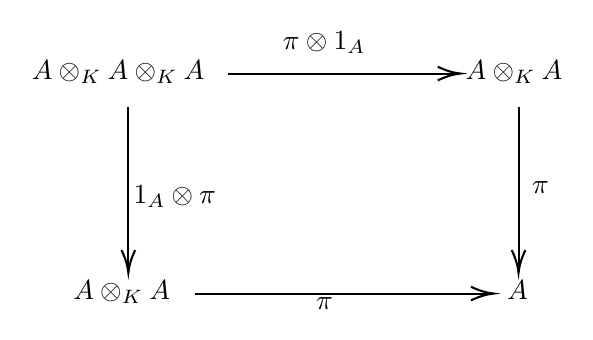
\begin{tikzpicture}[x=0.75pt,y=0.75pt,yscale=-1,xscale=1]
%uncomment if require: \path (0,476); %set diagram left start at 0, and has height of 476

%Straight Lines [id:da4446306867441949] 
\draw    (240,136) -- (350,136) ;
\draw [shift={(352,136)}, rotate = 180] [color={rgb, 255:red, 0; green, 0; blue, 0 }  ][line width=0.75]    (10.93,-3.29) .. controls (6.95,-1.4) and (3.31,-0.3) .. (0,0) .. controls (3.31,0.3) and (6.95,1.4) .. (10.93,3.29)   ;
%Straight Lines [id:da8073349826241552] 
\draw    (192,152) -- (192,230) ;
\draw [shift={(192,232)}, rotate = 270] [color={rgb, 255:red, 0; green, 0; blue, 0 }  ][line width=0.75]    (10.93,-3.29) .. controls (6.95,-1.4) and (3.31,-0.3) .. (0,0) .. controls (3.31,0.3) and (6.95,1.4) .. (10.93,3.29)   ;
%Straight Lines [id:da7945727275745025] 
\draw    (380,152) -- (380,230) ;
\draw [shift={(380,232)}, rotate = 270] [color={rgb, 255:red, 0; green, 0; blue, 0 }  ][line width=0.75]    (10.93,-3.29) .. controls (6.95,-1.4) and (3.31,-0.3) .. (0,0) .. controls (3.31,0.3) and (6.95,1.4) .. (10.93,3.29)   ;
%Straight Lines [id:da7073564025745236] 
\draw    (224,242) -- (366,242) ;
\draw [shift={(368,242)}, rotate = 180] [color={rgb, 255:red, 0; green, 0; blue, 0 }  ][line width=0.75]    (10.93,-3.29) .. controls (6.95,-1.4) and (3.31,-0.3) .. (0,0) .. controls (3.31,0.3) and (6.95,1.4) .. (10.93,3.29)   ;

% Text Node
\draw (144,128.4) node [anchor=north west][inner sep=0.75pt]    {$A\otimes _{K} A\otimes _{K} A$};
% Text Node
\draw (164,234.4) node [anchor=north west][inner sep=0.75pt]    {$A\otimes _{K} A$};
% Text Node
\draw (353,128.4) node [anchor=north west][inner sep=0.75pt]    {$A\otimes _{K} A$};
% Text Node
\draw (373,234.4) node [anchor=north west][inner sep=0.75pt]    {$A$};
% Text Node
\draw (265,114.4) node [anchor=north west][inner sep=0.75pt]    {$\pi \otimes 1_{A}$};
% Text Node
\draw (193,188.4) node [anchor=north west][inner sep=0.75pt]    {$1_{A} \otimes \pi $};
% Text Node
\draw (385,186.4) node [anchor=north west][inner sep=0.75pt]    {$\pi $};
% Text Node
\draw (281,242.4) node [anchor=north west][inner sep=0.75pt]    {$\pi $};


\end{tikzpicture}
\end{center}
is commutative. In this case the $K$-algebra $A$ has an identity if and only if there is a $K$-module homomorphism $I:K\to A$ such that the diagram 
\begin{center}


\tikzset{every picture/.style={line width=0.75pt}} %set default line width to 0.75pt        

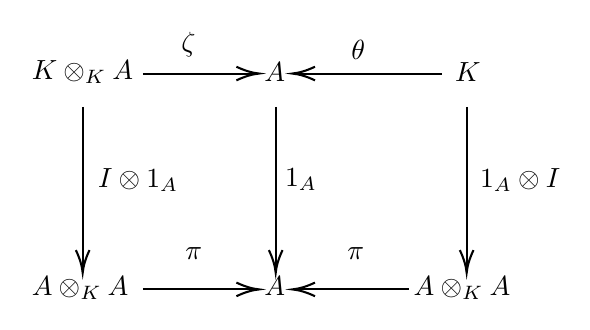
\begin{tikzpicture}[x=0.75pt,y=0.75pt,yscale=-1,xscale=1]
%uncomment if require: \path (0,476); %set diagram left start at 0, and has height of 476

%Straight Lines [id:da12856651333960145] 
\draw    (208,136) -- (262,136) ;
\draw [shift={(264,136)}, rotate = 180] [color={rgb, 255:red, 0; green, 0; blue, 0 }  ][line width=0.75]    (10.93,-3.29) .. controls (6.95,-1.4) and (3.31,-0.3) .. (0,0) .. controls (3.31,0.3) and (6.95,1.4) .. (10.93,3.29)   ;
%Straight Lines [id:da812781978806228] 
\draw    (352,136) -- (282,136) ;
\draw [shift={(280,136)}, rotate = 360] [color={rgb, 255:red, 0; green, 0; blue, 0 }  ][line width=0.75]    (10.93,-3.29) .. controls (6.95,-1.4) and (3.31,-0.3) .. (0,0) .. controls (3.31,0.3) and (6.95,1.4) .. (10.93,3.29)   ;
%Straight Lines [id:da531728198983914] 
\draw    (179,152) -- (179,230) ;
\draw [shift={(179,232)}, rotate = 270] [color={rgb, 255:red, 0; green, 0; blue, 0 }  ][line width=0.75]    (10.93,-3.29) .. controls (6.95,-1.4) and (3.31,-0.3) .. (0,0) .. controls (3.31,0.3) and (6.95,1.4) .. (10.93,3.29)   ;
%Straight Lines [id:da50625123814778] 
\draw    (208,240) -- (262,240) ;
\draw [shift={(264,240)}, rotate = 180] [color={rgb, 255:red, 0; green, 0; blue, 0 }  ][line width=0.75]    (10.93,-3.29) .. controls (6.95,-1.4) and (3.31,-0.3) .. (0,0) .. controls (3.31,0.3) and (6.95,1.4) .. (10.93,3.29)   ;
%Straight Lines [id:da7020069274231477] 
\draw    (336,240) -- (282,240) ;
\draw [shift={(280,240)}, rotate = 360] [color={rgb, 255:red, 0; green, 0; blue, 0 }  ][line width=0.75]    (10.93,-3.29) .. controls (6.95,-1.4) and (3.31,-0.3) .. (0,0) .. controls (3.31,0.3) and (6.95,1.4) .. (10.93,3.29)   ;
%Straight Lines [id:da7700224477602717] 
\draw    (364,152) -- (364,230) ;
\draw [shift={(364,232)}, rotate = 270] [color={rgb, 255:red, 0; green, 0; blue, 0 }  ][line width=0.75]    (10.93,-3.29) .. controls (6.95,-1.4) and (3.31,-0.3) .. (0,0) .. controls (3.31,0.3) and (6.95,1.4) .. (10.93,3.29)   ;
%Straight Lines [id:da2780316999628465] 
\draw    (272,152) -- (272,230) ;
\draw [shift={(272,232)}, rotate = 270] [color={rgb, 255:red, 0; green, 0; blue, 0 }  ][line width=0.75]    (10.93,-3.29) .. controls (6.95,-1.4) and (3.31,-0.3) .. (0,0) .. controls (3.31,0.3) and (6.95,1.4) .. (10.93,3.29)   ;

% Text Node
\draw (153,128.4) node [anchor=north west][inner sep=0.75pt]    {$K\otimes _{K} A$};
% Text Node
\draw (357,129.4) node [anchor=north west][inner sep=0.75pt]    {$K$};
% Text Node
\draw (153,232.4) node [anchor=north west][inner sep=0.75pt]    {$A\otimes _{K} A$};
% Text Node
\draw (265,129.4) node [anchor=north west][inner sep=0.75pt]    {$A$};
% Text Node
\draw (265,232.4) node [anchor=north west][inner sep=0.75pt]    {$A$};
% Text Node
\draw (337,232.4) node [anchor=north west][inner sep=0.75pt]    {$A\otimes _{K} A$};
% Text Node
\draw (225,114.4) node [anchor=north west][inner sep=0.75pt]    {$\zeta $};
% Text Node
\draw (307,118.4) node [anchor=north west][inner sep=0.75pt]    {$\theta $};
% Text Node
\draw (185,180.4) node [anchor=north west][inner sep=0.75pt]    {$I\otimes 1_{A}$};
% Text Node
\draw (275,180.4) node [anchor=north west][inner sep=0.75pt]    {$1_{A}$};
% Text Node
\draw (369,180.4) node [anchor=north west][inner sep=0.75pt]    {$1_{A} \otimes I$};
% Text Node
\draw (227,218.4) node [anchor=north west][inner sep=0.75pt]    {$\pi $};
% Text Node
\draw (305,218.4) node [anchor=north west][inner sep=0.75pt]    {$\pi $};


\end{tikzpicture}
\end{center}
is commutative, where $\zeta,\theta$ are the isomorphisms defined as in Theorem 5.54.
\end{theorem}
\begin{proof}
We first suppose that $A$ is a $K$-algebra. Then the map $A\times A\to A$ given by $(a,b)\mapsto ab$ induces a homomorphism of modules $\pi:A\otimes_KA\to A$. It is easy to verify that $\pi$ satisfy the condition. To prove the converse situation, define $ab=\pi(a\otimes b)$.\par
Now suppose $A$ has an identity. Then define $I:K\to A$ by $k\mapsto k1_A$, it is easy to verify that $I$ satisfy the condition. Conversely, define $1_A=I(1_K)$.
\end{proof}
\begin{note}\em
The homomorphism $\pi$ in Theorem 5.70 is called the \textbf{product map} of the $K$-algebra $A$. The homomorphism $I$ is called the \textbf{unit map}.
\end{note}
\begin{definition}
Let $K$ be a commutative ring with identity and $A,B$ $K$-algebras.\par
(i) A \textbf{subalgebra} of $A$ is a subring of $A$ that is also a $K$-submodule of $A$.\par
(ii) A (left, right, two sided) \textbf{algebra ideal} of $A$ is a (left, right, two sided) ideal of the ring $A$ that is also a $K$-submodule of $A$.\par
(iii) A \textbf{homomorphism} [resp. \textbf{isomorphism}] of $\mathrm{K}$-algebras $f:A\to B$ is a ring homomorphism [isomorphism] that is also a $K$-module homomorphism [isomorphism].
\end{definition}
\begin{note}\em
If $A$ is a $K$-algebra, then an ideal of $A$ need not be an algebra ideal of $A$. If, however, $A$ has an identity, then for all $k\in K$ and $a\in A$ we have 
$$
ka=k\left( 1_Aa \right) =\left( k1_A \right) a;\hspace{0.5cm}ka=\left( ka \right) 1_A=a\left( k1_A \right) ,
$$
whence for a left [resp. right] ideal $J$ in the ring $A$, we have $kJ=\left( k1_A \right) J\subset J$ [resp. $kJ=J(k1_A)\subset J$]. Therefore if $A$ has an identity, every ideal is also a algebra ideal.
\end{note}
The quotient algebra of a $K$-algebra $A$ by an algebra ideal $I$ is now defined in the obvious way, as are the direct product and direct sum of a family of $K$-algebras. Tensor products furnish another way to manufacture new algebras. We first observe that if $A$ and $B$ are $K$-modules, then there is a $K$-module isomorphism $\alpha:A\otimes_KB\to B\otimes_KA$ such that $\alpha(a\otimes b)=b\otimes a$ for all $a\in A,b\in B$.
\begin{theorem}
Let $A$ and $B$ be algebras [with identity] over a commutative ring $K$ with identity. Let $\pi$ be the composition 
$$
\left( A\otimes _KB \right) \otimes _K\left( A\otimes _KB \right) \overset{1_A\otimes \alpha \otimes 1_B}{\longrightarrow}\left( A\otimes _KA \right) \otimes _K\left( B\otimes _KB \right) \overset{\pi _A\otimes \pi _B}{\longrightarrow}A\otimes _KB,
$$
where $\pi_A$ and $\pi_B$ are the product maps of $A$ and $B$ respectively. Then $A\otimes_KB$ is a $K$-algebra [with identity] with product map $\pi$.
\end{theorem}
\begin{proof}
The verification is straight-forward by definition and we skip the details. Note that 
$$
\left( a_1\otimes b_1 \right) \left( a_2\otimes b_2 \right) =\pi \left( \left( a_1\otimes b_1 \right) \otimes \left( a_2\otimes b_2 \right) \right) =a_1a_2\otimes b_1b_2,
$$
thus if $A$ and $B$ has identities $1_A$ and $1_B$, then $1_A\otimes 1_B$ is the identity in $A\otimes_KB$, hence the second assertion is true in the theorem.
\end{proof}
The $K$-algebra $A\otimes_KB$ of Theorem 5.72 is called the tensor product of the $K$-algebras $A$ and $B$. Tensor products of algebras are useful in studying the structure of division algebras over a field $K$, which we shall introduce in the future.\par
\textbf{There are no exercises for this section.}